\documentclass[8pt, twoside, a5paper]{report}
\usepackage[usenames, dvipsnames, svgnames]{xcolor}
\usepackage{titlesec, blindtext, color, graphicx}
\usepackage[light,condensed,math]{kurier}
\usepackage[T1]{fontenc}
\usepackage{tcolorbox}
\usepackage{lipsum}

\tcbuselibrary{skins,breakable}
\usetikzlibrary{shadings,shadows}
\definecolor{GREEN}{rgb}{0, 0.5, 0.1}

%\usepackage{lmodern} % to remove warnings of size substitution
\usepackage[top=0.6in, bottom=0.6in, left=0.6in, right=0.4in]{geometry}

\tcbuselibrary{skins,breakable}
\usetikzlibrary{shadings,shadows}

\newenvironment{myexampleblock}[1]{%
    \tcolorbox[beamer,%
    noparskip,breakable,
    colback=LightGreen,colframe=DarkGreen,%
    colbacklower=LimeGreen!75!LightGreen,%
    title=#1]}%
    {\endtcolorbox}

\newcommand{\hsp}{\hspace{7pt}}
\newcommand{\hssp}{\hspace{3pt}}

\titleformat{\chapter}[hang]{\vspace{-2 cm}\huge\bfseries}{{\fontsize{50}{60}\selectfont \thechapter \hsp\textcolor{GREEN}{|}\hsp}}{0pt}{\huge\bfseries}
\titleformat{\section}[hang]{\large}{\thesection\hssp}{0pt}{\large\bfseries}

\newcommand{\authors}[1]{\small{#1}}
\newcommand{\italic}[1]{\textit{#1}}
\newcommand{\bold}[1]{{\bfseries #1}}
\newcommand{\code}[1]{{\tt #1}}
\newcommand{\mytitle}[1]{{\LARGE #1}}

\newcommand{\xqtlwb}{{\it x}QTL workbench }
\newcommand{\molgenis}{Molgenis} % don't use all caps, see journal guidelines
\newcommand{\xgap}{XGAP} % don't use all caps, see journal guidelines

\pagestyle{headings}
\renewcommand{\contentsname}{Table of content\vspace{-30pt}}

\begin{document}
\pagenumbering{arabic}
  \thispagestyle{empty}
  \begin{center}
  \mytitle{Methods and Software for Systems Genetics}\\
  \end{center}
\newpage
  \thispagestyle{empty}
  \noindent The work described in this thesis was carried out at the Groningen Bioinformatics Centre, University of Groningen, The Netherlands.
  This research was financially supported by the Centre for BioSystems Genomics (CBSG) and the Netherlands Consortium of Systems Biology (NCSB), both of which are part of the Netherlands Genomics Initiative / Netherlands Organisation for Scientific Research\\
  \vspace{130 mm}
  
  \noindent (c) 2013 by GBIC - Danny Arends\\
  Printed by:\\
  ISBN:\\
\newpage

\thispagestyle{empty}
\begin{center}
  \mytitle{Methods and Software for Systems Genetics}\\
    \vspace{10 mm}
  \bold{Proefschrift}\\
    \vspace{10 mm}
  Ter verkrijging van het doctoraat in de \\
  Wiskunde en Natuurwetenschappen \\
  aan de Rijksuniversiteit Groningen \\
  op gezag van de \\
  Rector Magnificus, dr. E. Sterken\\ 
  in het openbaar te verdedigen op \\
  Maandag 1 September 2013 \\
  om 12.00 uur \\
    \vspace{10 mm}
  door\\
    \vspace{10 mm}
  Derk Arends\\
    \vspace{10 mm}
  Geboren op 15 juli 1983\\
  te Zwolle
\end{center}

\newpage
\thispagestyle{empty}
\begin{tabular}{ l l }
Promotor:             & Prof. dr. R.C. Jansen \\
                      & \\
Co-Promotors:         & dr. F. Johannes \\
                      & dr. M. Swertz \\
                      & \\
Beoordelingcommisie:  & Prof. dr. \\
                      & Prof. dr. \\
                      & Prof. dr. \\
\end{tabular}
\tableofcontents

\chapter{Introduction}
\thispagestyle{empty}
\label{chap:introduction}

\emph{This first chapter introduces the reader to concepts such as gene, chromosome 
and DNA all the way up to Multiple QTL mapping (MQM) and Genome Wide Association Studies 
(GWAS). }

\null
\vfill
\newpage

\section{From pea plants to 'Big Data'}
Since the first genetic theories on the inheritance of phenotypes in pea plants were published by 
Gregor Mendel in 1865, the ongoing interest in the field has now resulted in an unprecedented stream 
of data to study Biology. The knowledge gain from Genetics research is huge as it has revealed how 
complex Biology actually is. 

Genetics research has shown how the activity of DNA is regulated by signals from all molecular levels, 
i.e. the genome, transcriptome, proteome, and metabolome. All these levels interact, and they are also 
modified by signals from the environment. Adding to the complexity, every level in the genetic paradigm 
has its own chemistry, functionality, and research technologies (See table \ref{tbl:overview}). Systems 
genetics is the research field in which we consider all these levels and interpret them together, within 
the context of DNA. Systems genetics aims to find the DNA variants underlying the variation that is 
seen on the higher molecular levels, all the way up to the phenotypes, for example seed quality in plants, 
and Crohn's disease in humans. 

The research fields of Genetics and Bioinformatics have been intertwined for several decades. Since the 
1980s it has become impossible to analyse data without using some form of computational assistance. This 
forces geneticists either to become 'computer savvy' or to collaborate with bioinformaticians. In practice, 
Genetics research has evolved into an interdisciplinary research domain. This thesis enters the field from 
the Bioinformatics perspective.

The ongoing stream of data that is being produced in the field of Systems genetics, poses several 
challenges to bioinformaticians. Data storage, computation on the data, and visualising the results, 
becomes increasingly harder when data sizes increase. For example, a clinician who has to deal with 
gigabytes of data while diagnosing a patient, requires access to good software. On a research level, 
understanding how a system works and reacts to different environments, allows modification of the system 
to better suit our needs or environmental requirements. The expected impact of such knowledge about DNA 
variation is to optimise  the breeding of livestock and crops, explore the genetic basis of human diseases, 
improved production of chemicals, and so forth. The use of computational tools in understanding how 
genetics and the environment intertwine is thus central to the field of Systems genetics and forms the 
basis how to deal with the large amounts of phenotype and genotype data. How we transform such data into 
usable knowledge is the main theme of this thesis.

\begin{table}[h]
  \centering
  {\footnotesize
  \begin{tabular}{ | c | l | l | }
    \hline
    {\bf Molecular level} & {\bf Molecule} & {\bf Technology}\\
    \hline
    \hline
\rowcolor{gray!35}    Genome          & DNA                & RFLP \cite{Lander:1986} \\
\rowcolor{gray!35}    Genome          & DNA                & SNP chips \cite{Hacia:1999} \\
\rowcolor{gray!35}    Genome          & DNA                & DNA sequencing \cite{Mardis:2008} \\
    \hline
    EpiGenome       & DNA methylation    & Bisulfite sequencing \cite{Hayatsu:2007} \\
    EpiGenome       & DNA methylation    & ChIP-on-chip \cite{Collas:2010} \\
    EpiGenome       & DNA methylation    & ChIP-Seq \cite{Park:2009} \\
    \hline
    \hline
\rowcolor{gray!35}    Transcriptome   & RNA          & Microarray \cite{Lashkari:1997}, Tiling array \cite{Lee:2013} \\
\rowcolor{gray!35}    Transcriptome   & RNA          & RNA-Seq \cite{Wang:2009}\\
    \hline
    Proteome        & Proteins     & 2D gel electrophoresis \cite{O'Farrell:1975}\\
    Proteome        & Proteins     & Mass Spectometry \cite{Deshaies:2001}\\
    Proteome        & Proteins     & Antibody protein chip \cite{Fasolo:2009} \\
    \hline
\rowcolor{gray!35}    Metabolome      & Metabolites  & Mass Spectometry \cite{Aebersold:2003} \\
\rowcolor{gray!35}    Metabolome      & Metabolites  & Nuclear magnetic resonance \cite{Espina:2009} \\
    \hline
  \end{tabular}
  }
  \caption[Overview]{Overview of current technologies to interrogate the molecular basis for life.}
    \label{tbl:overview}
\end{table}

Currently new data types are coming in more often than before. Previously geneticists dealt with mostly 
classical phenotypes and a limited number of genetic markers. Now we are able to map 1000s of traits onto 
millions of markers, creating not only more data, but also a more diverse kind of biological data. These 
new data also need to be considered when analysing and interpreting the outcome in terms of clinical and 
societal relevance. To merge all these inputs and give algorithms a unified view on such diverse data, 
requires generic data \rev{modeling}, and generators that use these models to create de-novo (web)-infrastructure, 
such as clusters, clouds and multi-core machines. 

The phenomenon of larger sample sizes, more data collection, and more intense computations, is a natural 
consequence of the data driven research which has increasingly become the focus of Systems genetics. Data 
driven research has caused the issue that we now call 'Big Data'. Making sense of this Big Data is increasingly 
difficult as it becomes harder to find clinical and societal relevant conclusions, while requiring ever 
larger computer facilities. This leads to increased societal costs, most notable in healthcare and industry. 
In the context of all these developments, it is important to consider more efficient usage of available 
resources, and avoid duplicate work effort. To contribute to this challenge we formed the following central 
question in this thesis:

How can computational bioinformatics help solving current 'Big Data' issues in Systems genetics?

\section{Approaches}

Recent developments in the computational infrastructure have created many new possibilities to deal with 
complex data in a powerful way. The impact of these developments is that all kinds of genetic concepts can 
now be tested. For example, 20 years ago the concept of Multiple QTL Mapping (MQM) was developed. This technique 
aims to compare all genetic markers to each other. At the time when MQM was conceptualised, it was computational 
very demanding. Because of the current increase of computational power, we are able to revisit MQM's methodological 
challenges and demonstrate that using high-throughput computational methodologies will allow us to solve research questions and 
do this in reasonable time. 

QTL mapping associates phenotype variation with genetic variation using appropriate statistical methods, such as 
t-tests, anova, and generalised linear models. MQM is a two-step procedure. First, it uses generalised linear models 
and backward selection of genetic cofactors to model the number of genetic factors underlying the phenotypes. In 
the second step, it uses the optimal model for QTL detection conditional to the selected cofactors. MQM is a superior 
technique compared to other methods for QTL mapping, as it allows detection of QTL in repulsion phase and performs 
with higher statistical power to detect phenotype to genotype associations. These advantageous characteristics 
are key to our decision to reintroduce the MQM algorithms into the Bioinformatics toolbox.

The Bioinformatics toolbox R/qtl \cite{Broman:2003, Arends:2010} is an open-source toolbox for mapping QTLs in inbred 
animals. It provides many QTL mapping routines and allows researchers to easily switch between statistical approaches, 
or test new approaches for QTL detection. Furthermore, it comes with a large user base and is de facto standard in 
the mouse QTL mapping community.

High throughput phenotyping provides us with data on thousands of phenotypes. Some of these phenotypes can be used 
as genetic marker because they show a major QTL effect. This leads to a situation in which we have a genetic 
map and an abundance of phenotypes which could be used to improve the map quality, by pinpointing all informative recombinations. 
This knowledge, combined with a lack of good genetic map creation software in the R/qtl package, has fuelled the development of the sensitive algorithm 
Pheno2Geno. It uses mixture \rev{modeling}, combined with a sensitive pre-selection approach. This results in faster 
genetic map creation as compared to other methods, and is the main reason for our ambition to add Pheno2Geno to R/qtl. 

QTL interactions are an \rev{important} area of interest in Systems genetics. For example, in recent years several papers were 
published on cell type or sex specificity of QTLs. Detection of these cell type specific QTLs has proven to be extremely 
difficult because it requires large sample sizes.  Meta-analysis, where we combine the samples from separate studies 
to improve power, is a prerequisite when studying cell type specific expression-QTLs (eQTLs). We noticed a lack of 
good software to meta-analyse these cell type specific QTLs in a genome wide setting. Furthermore, since cell type specific 
eQTL analysis is comparable to analysis that uses multiple environments, we propose to conceptualise cell abundance 
similar to an environment in which a QTL can be present or absent. Therefore, to consider such interactions, our toolbox 
also needs to be adjusted to support meta-analysis on genetical genomics experiments in which these QTL x Environment 
interactions are included.

All these advances are impossible without good infrastructure to funnel all the data streams into a network or image a 
biologist can understand. We noticed many separate tools for handling different facets of this ‘Big Data’ issue. Software 
such as database systems, web frameworks, computational tools, and APIs are available, but take considerable time to 
setup and master. Furthermore we noticed a lack of comprehensive software which combines all these tools into a 
comprehensible system, which is easy to use for a biologist.

New developments are common in Computational biology, and only the application of these new methodologies on biological 
datasets can show the value of the developed theories and software. Only when applications to real data demonstrate 
significant reductions in the amount of time needed to perform such analyses, or reveal new biological insights, we can 
conclude that a method is useful in the context of Systems biology. The value of methodologies and tools comes from the 
application of these methodologies and tools to real data. 

Considering these methodological Big Data issues in Systems genetics, the following sub-questions were formulated to 
guide the research: 

1. Whether and how can QTL be used in high-throughput trait data to computationally generate high (or higher) numbers of genetic markers to more accurately fingerprint samples? 

2. Whether and how can software for QTL analysis, in particular MQM for complex traits, be scaled up to cope with dense fingerprint/marker information and high-throughput trait data?

3. Design software infrastructure for storage of, and computation on high-throughput fingerprint/marker and trait data.

4. Which benefits of research questions 1-3 can be demonstrated on real high-throughput data, and which (Systems) biological insights does this reveal? 

\section{The first genetic theories (1800-1930)}
As this research project approaches 'old' genetic theories with new Bioinformatics tools, it is relevant to place 
them in their historic context. The research field of genetics is relatively old, as it is founded when Gregor 
Mendel publishes his work on the inheritance of phenotypes in pea plants. His work, described in 'Versuche \"uber 
Pflanzen-Hybriden' in 1865-1866 \cite{Mendel:1866}, gives us Mendel's Laws of Inheritance. He observed that crossing 
two plants with different flower colours leads to an offspring population with predictable colour ratios. He 
postulated the idea of heredity units and stated that each individual carries two of these, which results in a 
single phenotype. Each heritable unit is received from one of the parents, but which one is passed on to the 
offspring is random. Mendel formulated this principle as First Law on Segregation: if two units are not equal, 
a dominant unit (colour 1) overrules another unit (colour 2 - recessive). 

Additional to studying colour, Mendel also studied other phenotypes in the pea plants besides colour. Now we know 
that Mendel was fortunate to select phenotypes which are caused by a single gene and are inherited independently. 
Mendel also observed this phenomenon of independent inheritance when comparing the inheritance of multiple 
phenotypes. He concluded that a unit of inheritance is passed from parent to offspring in an independent fashion, 
that is, independent  from other phenotypes that are inherited. This principle is known as Mendel's Second Law 
on Independent Assortment.

The relevance of Mendel's inferences was not fully recognised until 30 years later, when his work was rediscovered 
by Hugo de Vries, Carl Correns, and Erich von Tschermak. They (re)defined the rules for Mendelian Genetics \cite{deVries:1889}. 
In doing so, they provided biologists for the first time with a mathematical framework to study heritability of 
phenotypes caused by a single genetic unit.

Twenty years after the rediscovery of Mendel's Laws, careful observations of Thomas Hunt Morgan introduced in 1913 
an addition to Mendel's theoretical work. He observed that some phenotypes in his Drosophila melanogaster mutant 
flies are inherited together. This is in conflict with Mendel's Laws, stating independent inheritance of genetic 
units. Morgan called this phenomenon genetic linkage. A specific situation arises when phenotypes are linked to 
the sex of the animal. This is called sex based inheritance \cite{Morgan:1915, Morgan:1916}.

Mendel worked on plants, while Morgan worked on fruit flies. Although the genetic basics are very similar, the sex 
linked inheritance is not observed in most plants as they are usually male and female at the same time. Currently 
four plant families \rev{(asparagus, hops, papaya and silene)} have been discovered that developed sex chromosomes acting 
similar to the sex chromosomes in animals \cite{Ming:2007}. Interestingly, these phenotypes do not follow Mendel's 
Second Law, as the traits are not inherited independently, but are linked to the sex phenotype. 

The concept of genetic linkage is commonly explained as beads on a string, in which multiple genetic units are 
linked together.  Two beads close together are tightly linked and almost always inherited together. In contrast, 
two beads that are far apart are less linked and can be separated by meiosis. Different strands are inherited 
independently, and thus allow Mendelian inheritance by two beads on two different strings. 

Sturtevant, one of Morgan's students, used his mentor's linkage theory between phenotypes as a measure of distance 
between units of inheritance. He created the first genetic map of Drosophila Melanogaster in 1916, 40 years before 
the discovery of the DNA molecule \cite{Morgan:1916}, and at a time when molecular mechanisms were still unknown. 
Sturtevant's genetic map, based on phenotypes, was used to study Genetics based on careful observation of the 
segregation of phenotypes in large populations of flies, and then determining the distance between the units of 
inheritance relative to other phenotypes. Observations showed that sometimes the link between two phenotypes is 
broken. The amount of times this is observed in a population, is taken as a measurement of distance between the 
two phenotypes. For example, when we have measured 200 phenotypes in crosses, we can estimate which belong together 
on the same chromosome, as these are the ones which are found together more often than randomly expected. Further 
exploration of the data can indicate the order of the phenotypes on the map.

Intermezzo - The same method to measure distances is nowadays used to construct genetic maps on phenotypes in Pheno2Geno. 
It differs from methods using genotypes, i.e. SNP chips, as they require DNA sequencing data. Such methods are more 
expensive because first the phenotypes are measured, followed by the genotypes. Pheno2Geno applies data of measurements 
of distance between phenotypes to subsequently define the genotypes, without a second measure.  

In 1918 Ronald A. Fisher published a paper entitled 'The Correlation Between Relatives on the Supposition of 
Mendelian Inheritance'. The paper demonstrates that a large number of small effects from discrete genetic 
units eventually add up to the continuous phenotypes observed \cite{Fisher:1918}. Fisher proposed to unify all 
phenotypes, discrete and continuous, in one model. Mendel's theories could only explain dichotomous phenotypes, 
e.g. yellow versus green, but the phenotypes that were most interesting to researchers, are continuous. As 
Mendel's theory did not apply to these, his work was ignored in favour of other theories. Fisher developed 
mathematical approaches to explain continuous phenotypes, such as human stature, and showed that they follow 
Mendel's Laws. He proposed that geneticists had to search for a number of small effect loci. Summation of 
these small dichotomous effects from many genetic units on a population scale would add up to the observed 
normal distribution. (This theory was only proven after Watson \& Crick and the discovery of DNA and genes).

With this observation we move to the next section, in which a book by R. Fischer again plays a major role in 
the development of population genetics.

\section{DNA and QTLs (1930-1990)}



In 1930, Fisher published the book 'The Genetical Theory of Natural Selection' \cite{Fisher:1930}. Fisher describes 
how Mendelian genetics is consistent with the idea of evolution by natural selection. His reasoning turned out 
to remove one of the last barriers for large scale adoption of Mendel's theories in Biology. The subsequent discovery 
of DNA as the carrier of heritability by Avery, MacLeod and McCarty in 1944 \cite{Avery:1944}, and the discovery of 
its structure by Watson and Crick in 1953 \cite{Watson:1953}, revealed the long sought-after molecular basis for Genetics. 

\begin{wrapfigure}{r}{0.5\textwidth}
  \centering
  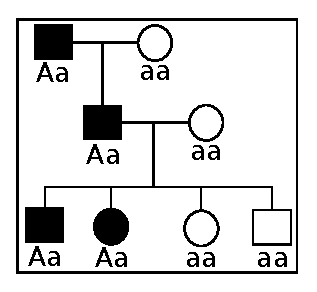
\includegraphics[width=0.4\textwidth]{eps/image_1_2.eps}
  \caption[Example of pedigree based linkage analysis.]
    {Example of a hypothetical pedigree on which linkage analysis can be performed. Here we show a 
    hypothetical pedigree of individuals within a family (2 generations), squares represent 
    male individuals while circle are females. The phenotype is shown encoded by the fill 
    color of the shape (Black = affected, White = not affected).  In this example pedigree, 
    the "A" allele segregates with the disease. It is shared identical-by-descent in all 
    affected individuals. }
    \label{fig:pedigree}
\end{wrapfigure}


After the discovery of restriction enzymes by Luria and Human \cite{Luria:1952} it was possible to cut and paste pieces 
of DNA. This allowed to experimentally work with DNA and investigate the different (lengths of) fragments produced, 
create new combinations of known DNA, and even novel DNA sequences to study the heritability of phenotypes. In 1970 
the first techniques were developed to sequence DNA. The first approach used two-dimensional chromatography, and was 
followed by fluorescence based sequencing methods \cite{Pettersson:2009}.

By the end of the 1980s everything was there for the next big step in Genetics. Three papers were published which detailed 
the use of Restriction fragment length polymorphism (RFLP) linkage maps to localise genes responsible for variation in 
quantitative phenotypes. These three papers by David Botstein and Eric Lander \cite{Lander:1986, Lander:1987, Lander:1989} 
form the basis for modern day linkage analysis and genome wide association studies. This allowed, for the first time in 
history, the direct association of DNA with its effect on a phenotype. 

These tools are used by geneticists and bioinformaticians to identify the region of DNA underlying phenotypes or diseases 
(if any). These regions are in themselves already interesting because they provide targets to optimise the phenotype (e.g. 
when improving plant yield), or for developing therapies/drugs for human diseases. Two methods of QTL analysis are applied 
in searching  DNA regions, i.e. linkage analysis and association analysis. 


\emph{Linkage analysis} is the DNA technology to trace parents and offspring/children. It is used to build so called genetic 
family trees or pedigrees (See fig. \ref{fig:pedigree}) in which segregation of a phenotype (for example a disease) is 
displayed. When we find a genetic region that co-segregates with the disease, we can assume the DNA and the disease are 
linked, allowing assessment of the strength of the observed linkage \cite{Rosyara:2009}. When experimental crosses derived 
from inbred parents are used, the need to build up complex pedigrees is avoided, while retaining the advantage of being able 
to trace back the DNA to the founder strains. Inbred populations also provide high statistical power at the cost of reduced 
resolution for QTL mapping \cite{Jansen:2001a}. This reduced resolution is caused by the lack of recombination in small 
populations (20 to 1000 individuals). 


\begin{wrapfigure}{r}{0.5\textwidth}
  \centering
  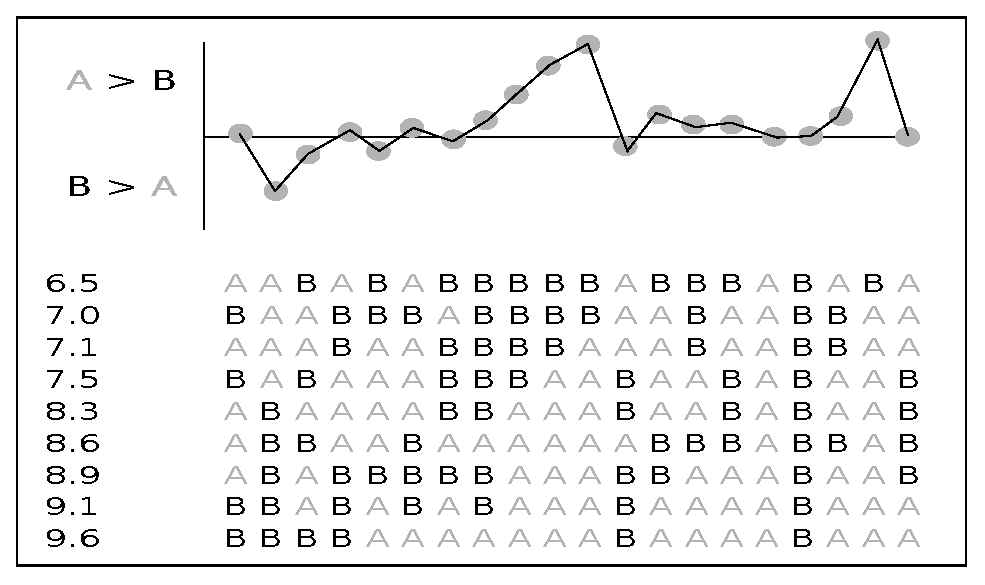
\includegraphics[width=0.5\textwidth]{eps/image_1_1}
  \caption[Effect scan across the genome.]
    {An example of how effect scans are performed using a single phenotype measured on 9 individuals (colored numbers)
    and genotypes represented by rows in the matrix (A or B). 20 markers (columns) were assessed: A and B are genetic 
    variants obtained from either parental or maternal line. }
    \label{fig:effectscan}
\end{wrapfigure}

An example of a basic effect scan using linkage analysis is shown in Figure \ref{fig:effectscan} At each marker the mean of 
the phenotype for AA and BB is calculated, and the difference is plotted per marker. This gives an initial indication which 
markers may be relevant biomarkers for the phenotype of interest.

\emph{Association analysis} can be applied in outbred, or natural populations when tracking the origin of the DNA is difficult 
or impossible. Molecular markers still allow to find information about the underlying DNA. We can use e.g. single nucleotide 
polymorphisms (SNPs) to associate a phenotype with the genetic marker \cite{Mehta:2013} The advantage of this approach is that 
the resolution is very high (around 200 - 300 kb in humans \cite{HapMap:2005}) because outbred populations have a high number of 
recombinations, as compared to experimental populations created from inbred lines. At the down side is that the large number of markers reduces the statistical 
power to detect effects as the result of multiple testing. Heritable phenotypes can be mapped to genomic locations using a 
combination of DNA restriction enzymes, Mendel's inheritance laws, and Hunt's linkage theory. Together these methodologies and 
theories provide the experimental and statistical background to analyse heritability in any population.

Linkage analysis and association analysis, both developed in the 1980s, are still the foundation of population genetics research. 
More sophisticated tools and algorithms have been developed and implemented, but the basic theoretical concepts are the same. 
Some of these more advanced methods are discussed in the next section to sketch a background for the work presented in this 
thesis. 

\section{From phenotypes to genetical omics and GWAS (1990-2010)}

The basis of an observed phenotype expression is often more complex than a single causative gene \cite{Sinha:2006, 
West:2007}. To model these more complex situations where multiple regulators are influencing gene expression levels requires extension of 
the basic model for QTL mapping. Extending the model is done by incorporating sources of variation as co-factors. This 
allows us to associate/partition the observed variance to either environmental factors (E) or genetic loci (G). The method 
is to include additional genetic components into the model, and then scan for QTLs conditional on these other genetic effects. 
This is the basic principle of Multiple QTL Mapping (MQM). MQM belongs to a family of QTL mapping methods, that includes 
Haley-Knott regression \cite{Haley:1992} and composite interval mapping (CIM) \cite{Zeng:1994}. MQM combines the strengths 
of generalised linear model regression with those of interval mapping \cite{Jansen:1993, Jansen:1994b}.

During the first years of QTL mapping, the genetic maps were of poor quality, with a lot of missing marker data and large 
gaps between markers. As a solution to this problem interval mapping was developed. Interval mapping uses prior knowledge 
about linkage in inbred populations to map QTLs between two genetic markers. Hidden Markov models (HMMs) are used to estimate 
the unobserved genotypes in the population based on the surrounding genotype observations, thereby improving the QTL 
mapping resolution \cite{Jansen:1993, Zeng:1994}.

Genetical genomics is the concept that deals with endophenotypes (RNA, protein and metabolite abundance) as if they were 
common phenotypes. They are mapped in bulk to the genome, in a way similar to classical phenotypes \cite{Jansen:2001a}. 
Natural occurring variation and new omics tools allow us to track variation from the genotype all the way up to the classical 
phenotypes (see Table \ref{tbl:overview} for a short overview of methods). Tracing the effects of variation from genome 
to phenotype allows Genetics to go from individual QTLs to a system-wide approach of analysing QTLs at all known molecular 
levels. This approach is called Systems genetics \cite{Threadgill:2006, Nadeau:2011}

Studies in model organisms have shown high heritability's for endophenotypes, such as gene expression, making these phenotypes 
ideal targets for QTL mapping \cite{Brem:2002, Yvert:2003, Morley:2004}. In 2003 R/qtl was developed to provide reference 
implementations for QTL mapping. R/qtl is an extensible, interactive Software/R package to map quantitative trait loci (QTL) 
in experimental crosses. It is implemented as an add-on package for the freely available and widely used statistical 
language/software R \cite{R:2009} The main focus of R/qtl is to provide the mouse community with different QTL mapping 
methodologies, and allow to deal with the aberrant segregation X chromosome. Furthermore\rev{,} it supports different types of 
inbred populations such as backcross (BC), F2, Recombinant inbred lines (RIL) and 4-way RILs \cite{Broman:2003}.

When mapping gene expression or protein abundance current knowledge of protein and DNA sequence allows us to locate their 
template on the genome. If QTL mapping resolution is high enough, we can even distinguish between traits mapping in the 
proximity of their respective gene (cis-eQTL) or to other regions in the genome (trans-eQTL). This information can be summarised 
into so called cis-trans plots, where the X-axis is the location of the eQTL and the Y-axis the genetic location of the trait. 
Often so called trans-bands are observed, hotspots of many trans- eQTL mapping to a common region in the genome \cite{Breitling:2008a}. 
These are used to infer biological meaning and reconstruct co-expression and/or co-regulatory networks.

In the last decade Genome Wide Association Studies (GWAS) have identified thousands of genetic variants that are associated 
with human disease \cite{Hindorff:2009}. For reliable results GWAS needs a large cohort of genotyped and phenotyped individuals. 
Large consortia are working together to gather large amounts of human expression data from many different tissues. These data 
are then used in meta-analysis leading to eQTL GWA studies with even larger sizes (5000+ individuals) \cite{Lude:2011}, leading 
to more reliable results and enabling discovery of new modifiers of human gene expression. It is now recognised that many factors, 
such as effects on intermediate molecular phenotypes, influence the relationship between genotype and the eventual development 
of disease. It has also been observation that many of the disease predisposing variants are non-coding, which suggests that 
these variants have a regulatory function. Furthermore\rev{,} it has been shown that many disease predisposing variants (e.g. single 
nucleotide polymorphisms (SNPs)) affect the expression of nearby genes (i.e. cis-eQTLs) \cite{Zeller:2010, Lude:2011, Powell:2012}

Currently data are being produced on all these bio-molecular levels on an unprecedented scale. Advances in sequencing technology, 
transcriptomics, proteomics, and metabolomics allow data collection on a scale much larger than before \cite{Editorial:2009, Shah:2013}. 
With this increasing scale of experimental data being produced in the lab, it will not be sufficient to have analysis software as 
simple downloads, because the researcher will also need sizable compute and storage power \cite{Schadt:2010}. How this increasing 
demand for storage and computational power can be satisfied in the future remains an open question. 

Federate computing providers may help researcher in their need for big computing solutions in the near future. However, this is also 
not a universal solution, as the speed of data production is currently higher than the speed of computing improvements 
\cite{Moore:1998, Editorial:2009, Shah:2013}. Other solutions are sought by corporations and universities, who have started to combine 
their efforts and set up shared infrastructure. They attempt to deal with the necessary increase in compute power and to save 
overhead costs such as maintenance and electricity. The next section takes a closer look at the two main infrastructural developments 
for large scale computation: cluster and cloud computing.

\section{Cluster and cloud computing (since 1980)}
A cluster is a collection of computers dedicated to solve a computational task by divide and conquer \cite{Silva:1999, Qiu:2010}. It 
basically means that a large supply of relatively homogeneous software is available on demand, including suitable compute and storage 
hardware. The hardware resources are divided by an internal scheduling system to facilitate efficient conduct of different tasks from 
various users. These users generally have little control over the computational environment, as the cluster administration and the 
scheduling system constrain its use. Computing clusters are fashioned to serve various types of hardware, such as:

Ad-hoc networks \rev{are} composed of many heterogeneous and relatively cheap systems such as: \rev{FPGAs, CPUs and/or ARM cores.}

Dedicated computer clusters, such as TARGET or national GRIDs, \rev{are} usually a homogenous system of Linux machines is used for computational tasks\rev{.}

Video card cluster for linear algebra, utilizing the power of many simple GPU cores for dedicated tasks.

Compute clusters do not have to be homogeneous in nature, but in many cases homogeneity is required to provide users with a stable 
computational environment to perform their tasks. Additionally the hardware can limit the usage of a cluster to a certain range of 
computational tasks, such as GPUs or dedicated ARM cores.

The term 'cloud' is used in many different ways, and there is little consensus on what a cloud exactly is \cite{Foster:2008}. Essentially 
it \rev{means a user} has software available on demand, on suitable compute and storage hardware, and is charged for the time that it is 
being used. The leading cloud provider is currently Amazon, who has introduced the concept of a virtual Linux machine. This is a virtual 
Linux pre-initialised compute server, that is hosted within some large compute infrastructure, providing the user customised freedom for 
a reasonable price \cite{Trelles:2011}.

Many commercial, national and local compute centres are now also developing cloud compute server capacity. These virtual machines are 
therefore easy accessible provisions to distribute software and computation without the need for all participating computational nodes 
to install software. Thus, the infrastructure is specified jointly \cite{Foster:2008} but for the actual computation every partner can 
be private with their own data. This approach grants enormous computational power to everyone with minimal preparation - once a shared 
image is finalised \cite{Krampis:2012}.

\rev{The} setup of such a compute cloud is not trivial and several initiatives are underway to ease this process. An example is the Debian Med 
\rev{initiative that} organised workshops where bioinformatics tested a packaging system as a method to create a cloud. The initiative is 
considered a seed for an image to then be publicly shared.

Using this method the cloud infrastructure can be transferred to local computer clusters when necessary. Every participant has access 
to the server and can grant access to collaborators without having to pay the hosting fees. When complete, the server image can be 
ported to cloud providers, such as Amazon or Rackspace, to be reused by other researchers.

%\begin{figure}[h!]
% \centering
%    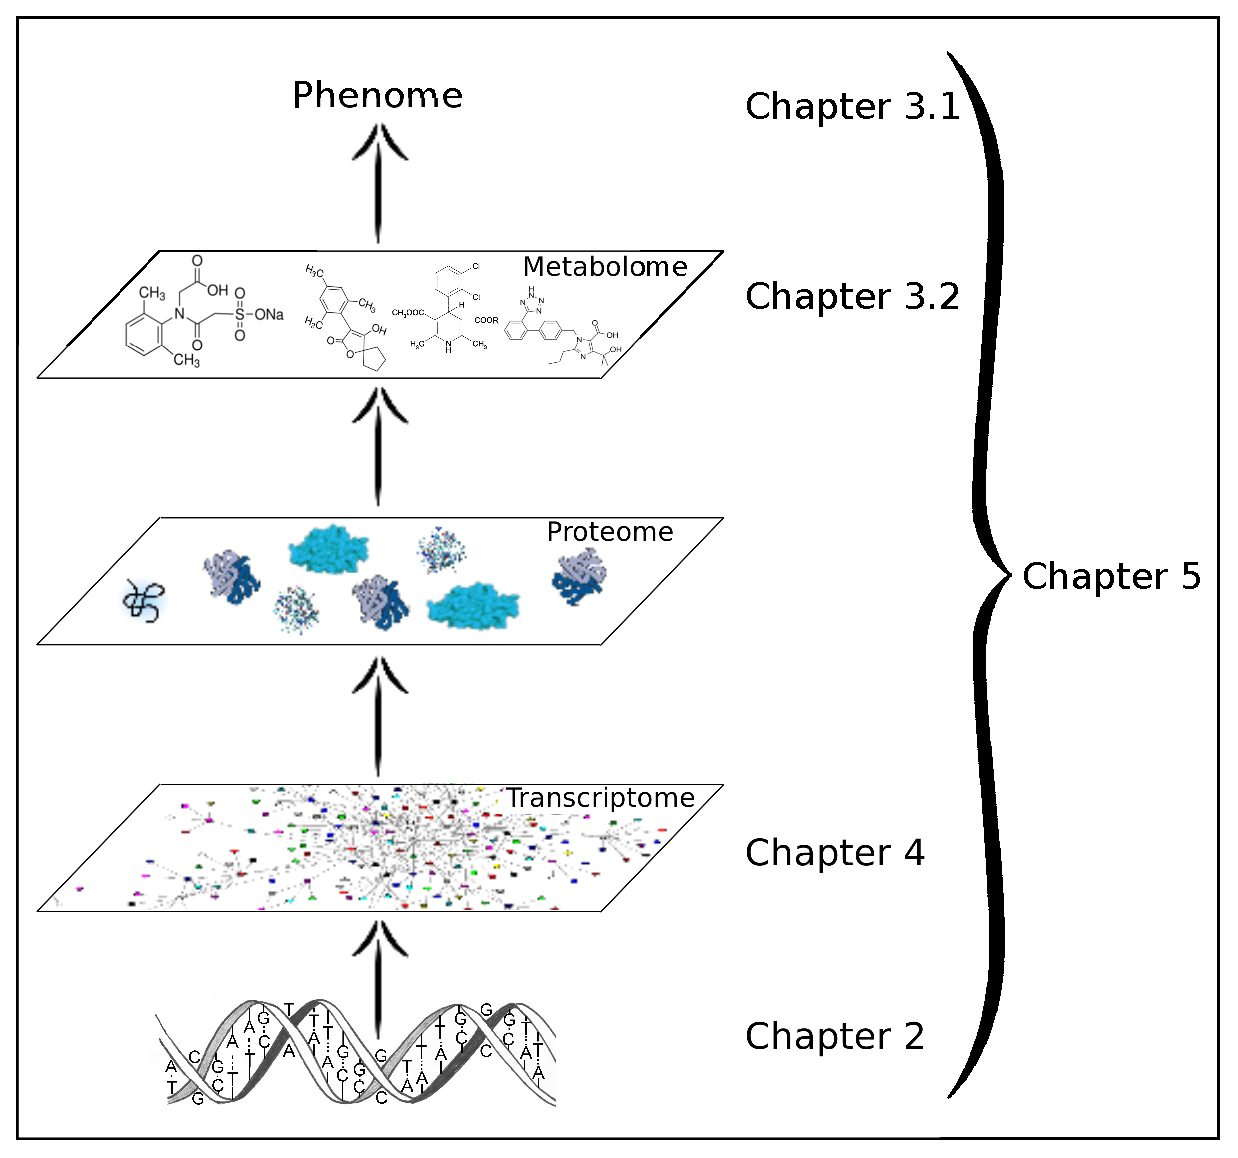
\includegraphics[width=0.6\textwidth]{eps/image_1_3}
%  \caption[ThesisLayout.]
%    {Schematic figure showing to which molecular level each chapter is related. Each molecular 
%    level here depicted are drawn from genome (bottom) to phenome (top), arrows indicate 
%    how genetic information is transferred from level to the level as by the current by 
%    the biological 'dogma'.}
%    \label{fig:layout}
%\end{figure}

%\section{Thesis contributions (2010-2014)}
%This thesis advocates that using smarter more optimized algorithms such as Pheno2Geno 
%(Chapter \ref{chap:pheno2geno}) or Multiple QTL mapping (Chapter \ref{chap:mqm}), 
%combined with taking advantage of modern shared computational infrastructure can provide 
%a solution to the 'Big Data' challenge. Federated computing, and collaborative research 
%requires tools such as xQTL workbench (Chapter \ref{chap:xqtlwormbench}) to work 
%together and avoid duplicate efforts.

%The following chapters will highlight in more detail the different contributions made to 
%the field of systems genetics during the 4 years of my PHD research at the University of 
%Groningen. A schematic overview connecting chapters to the different bio molecular levels 
%can be found in Figure \ref{fig:layout}.

%Chapter \ref{chap:pheno2geno} details how Pheno2Geno an R package was developed for 
%the high-throughput generation of genetic markers and maps from molecular phenotypes. 
%Pheno2Geno selects suitable phenotypes that show clear differential expression in the founders. Pheno2Geno 
%uses mixture modeling to select phenotypes showing segregation ratios close to the 
%expected Mendelian segregation ratios and transform them into genetic markers suitable 
%for map construction and/or saturation. Pheno2Geno analyzes the candidate genetic 
%markers and excludes those showing multiple QTL, epistatically interacting QTL, and QTL 
%by environment interactions to provide a set of robust markers for QTL mapping protecting 
%against genetic markers from a non genetic origin.

%Chapter \ref{chap:mqm} highlights the integration of the Multiple QTL mapping algorithm 
%into R/qtl. In sections (\ref{chap:mqm}.1 and  \ref{chap:mqm}.2) we show the performance 
%of MQM on experimental data from a cross of \emph{A. thaliana} Bayreuth x Shahdara. We 
%focus on the developing seeds in this cross and try to find genetic factors underlying 
%changes we observed in the phenome and metabolome.

%Chapter \ref{chap:ctlmapping} -  Shows our current work on understanding differences in 
%correlation observed when mapping two traits onto the genome. We show that there is a high 
%overlap between CTL mapping and using an G:E interaction model, and apply this interaction 
%model to data from a human genome wide association study (GWAS). We detect cell type specific 
%eQTL in whole blood for neutrophils, and show that low effect QTLs observed in samples can be explained by 
%compensating for the relative number of neutrophils observed, or predicted. Cell type specific 
%eQTL analysis will improving our power to detect QTLs and enables us to assign cell type labels 
%to observed \emph{cis}-eQTL effects.

%Chapter \ref{chap:xqtlwormbench} - Details our work to provide infrastructure for the Life 
%Sciences. We advocate the use of Generators to create software and propose a data model (XGAP) 
%to store phenotype and genotype data. Combining these two approaches we developed: xQTL 
%workbench a scalable web platform for the mapping of quantitative trait loci (QTLs) at 
%multiple levels such as gene expression (eQTL), protein abundance (pQTL), metabolite 
%abundance (mQTL) and phenotype (phQTL) data. Popular QTL mapping methods for model organism 
%and human populations are accessible via the web user interface. Large calculations scale %
%easily on to multi-core computers, clusters and cloud computing.

%There are enough subjects to cover in this thesis. We start by improving the genetic map for 
%our model organism \emph{A. thaliana}. We introduce Multiple QTL mapping (MQM), which we use 
%to find genetic loci involved in seed quality traits in \emph{A. thaliana}. We expand our 
%methodology by looking at different environments and realize cell type is just another 
%factors which can be handled in a similar way as environments. Finally we discuss the 
%implications of the ever increasing stream of raw data available through new technologies and 
%our vision (xQTL workbench) on how to handle big data and avoid duplicated effort by a 
%collaborative research platform.



\chapter{High throughput generation of genetic markers}
\thispagestyle{empty}
\label{chap:pheno2geno}
\emph{Using prior knowledge about phenotypes and how they are transfered during 
reproduction allows us to create phenotype based genetic markers. We can use 
these derived markers to saturate existing genetic maps or create them de-novo 
when enough data is available. Pheno2Geno was developed to use a sensitive 
pre-selection and mixture modeling approach to improve performance. The package 
is designed to be fast enough to make use of data from diverse data sources such 
as: microarrays, tiling arrays and/or RNA-Seq experiments. Using data from tiling 
arrays we were able to improve the genetic map resolution of an A. thaliana 
Recombinant Inbred Line (RIL) derived from a Bayreuth (Bay-0) x Shahdara (Sha) cross.}

\null
\vfill

\begin{myexampleblock}{Under review:}
  \authors{Konrad Zych*, K. Joeri van der Velde, Ronny V. L. Joosen, Wilco Ligterink, Ritsert C Jansen and Danny Arends}\\
  \emph{Pheno2Geno - High throughput generation of genetic markers and maps from molecular phenotypes}\\
  \bold{BMC Bioinformatics} (XXXX)
\end{myexampleblock}
\newpage

\section{Pheno2Geno}
Genetic markers and maps are instrumental for quantitative trait locus (QTL) mapping in segregating 
populations. The resolution of QTL localisation depends on the number of informative recombinations 
in the population and how well these recombinations are tagged by markers. Thus larger populations 
and denser marker maps perform better at detecting and locating QTLs. In practice, marker maps are 
often still too sparse. However, maps can be saturated or even be derived \emph{de-novo} from high-
throughput omics data, such as gene expression, protein or metabolite abundance data. This is because 
molecular phenotypes are influenced by genetic variation and they will show a clear multimodal 
distribution due to major QTL effects, such information can therefore be converted into useful 
genetic markers.

The Pheno2Geno R package is developed for high-throughput generation of genetic markers and maps from 
molecular phenotypes. Pheno2Geno selects suitable phenotypes that show clear differential expression 
in the founders. Pheno2Geno uses mixture modelling to select phenotypes showing segregation ratios 
close to the expected mendelian segregation ratios and transform them into genetic markers suitable 
for map construction and/or saturation. Pheno2Geno analyses the candidate genetic markers and excludes 
those showing multiple QTL, epistatically interacting QTL, and QTL by environment interactions to 
provide a set of robust markers for QTL mapping protecting against genetic markers from a non genetic 
origin.

We demonstrate our tool using gene expression data of 370.000 transcripts in 164 \emph{A. thaliana} 
Recombinant Inbred Lines (RILs). Pheno2Geno is able to saturate the existing genetic map decreasing 
the average distance between markers from 7.1 cM to 0.89 cM, close to the theoretical limit of 0.6 cM, 
pinpointing almost all of the informative recombinations in the population. Pheno2Geno is also able 
to created a \emph{de-novo} map from the gene expression data that is twice as dense as the original 
genetic map.

The Pheno2Geno package offers high-throughput \emph{de-novo} map construction and saturation of 
existing genetic maps. Processing of the showcase dataset takes less than 30 minutes on an average 
desktop PC. Pheno2Geno improves QTL mapping results at no additional laboratory cost and with 
minimum computational effort. Pheno2Geno results are formatted for direct use in R/qtl, the leading 
R package for QTL studies. Pheno2Geno is freely available on CRAN under GNU GPL version 3.

\section{Background}
QTL mapping \cite{Lander:1989} is a powerful approach used in population analysis to link 
genetic variation to phenotypic variation. It requires polymorphic genetic markers positioned 
on a genetic map. Phenotypes showing a dichotome 0/1 distribution with approximate equal 
proportions in, say, a RIL population can be used as genetic markers: genotypes can be 
called by connecting the 0/1 to the parental strains A/B. Such markers can then be used 
for de-novo construction of the genetic map or for saturation of a known genetic map 
\cite{West:2006, Truco:2013}.

Continuous (non-dichotome) phenotypes can also be used as markers if they show a major QTL: a 
major QTL will cause the phenotype to show a clear multimodal distribution to which a mixture 
models can be fitted \cite{Jansen:1993, Jansen:2001a}. Posterior probabilities derived from 
mixture modelling are used for genotype calling. Such approaches have been used for up to 
1,200 molecular phenotypes \cite{Gort:2010}.

Here, we scale up the mixture model approach for non dichotome phenotypes in order to make 
analysis of hundreds of thousands of molecular phenotypes feasible e.g. gene expression data.

Genetic maps created by Pheno2Geno can be easily used for QTL mapping: the package provides 
output structures compatible with R/qtl, the leading R package for QTL analysis in 
experimental crosses \cite{Broman:2003, Arends:2010}. Pheno2Geno allows users to 
explore and compare resulting maps with their favourite genome browser. Maps can be saved
as a GFF (General Feature Format) file that is supported by most genome browsers.

\begin{figure}[h!]
  \centering
  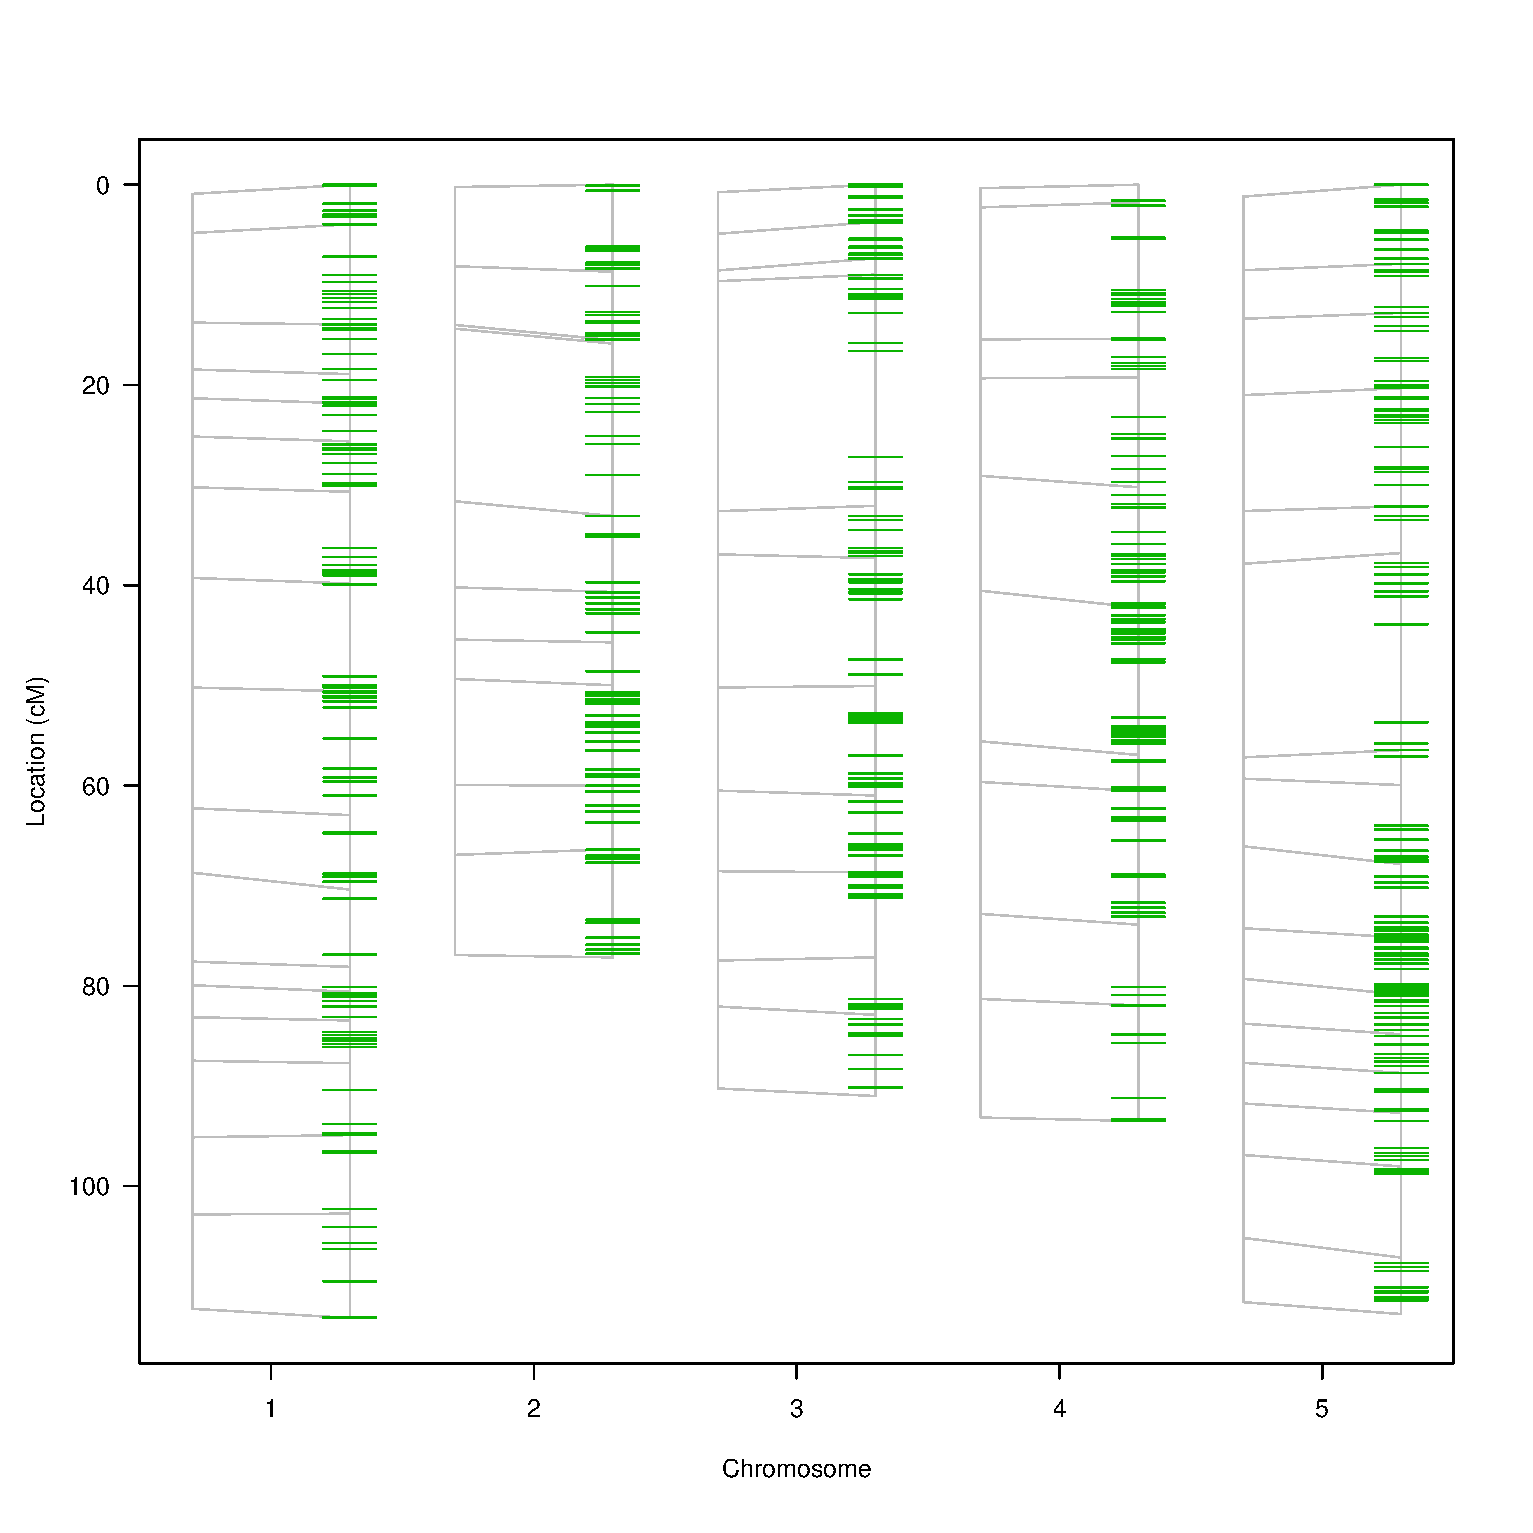
\includegraphics[keepaspectratio,width=0.8\textwidth]{eps/image_2_1.eps}
  \caption[Map comparison]{Map comparison plot drawn using R/qtl function \emph{plot.map} \cite{Broman:2003, Arends:2010}. For 
          each of the chromosomes the original map (left) and the saturated map (right) are plotted. Lines are drawn
          to connect markers.  Markers that exist in just one map and not the other are indicated by short line 
          segments, on one side or the other, that are not connected across. Before plotting, both maps were 
          re-estimated using the R/qtl function \emph{est.map}. The original map consists of 5 chromosomes and 69 
          markers at an average distance of 7.1 cM. The saturated map consists of the original 69 markers plus 497 
          expression-based markers at an average marker distance of 0.89 cM.}
          s\label{fig:mapcomparison}
\end{figure}

\begin{figure}[h!]
  \centering
  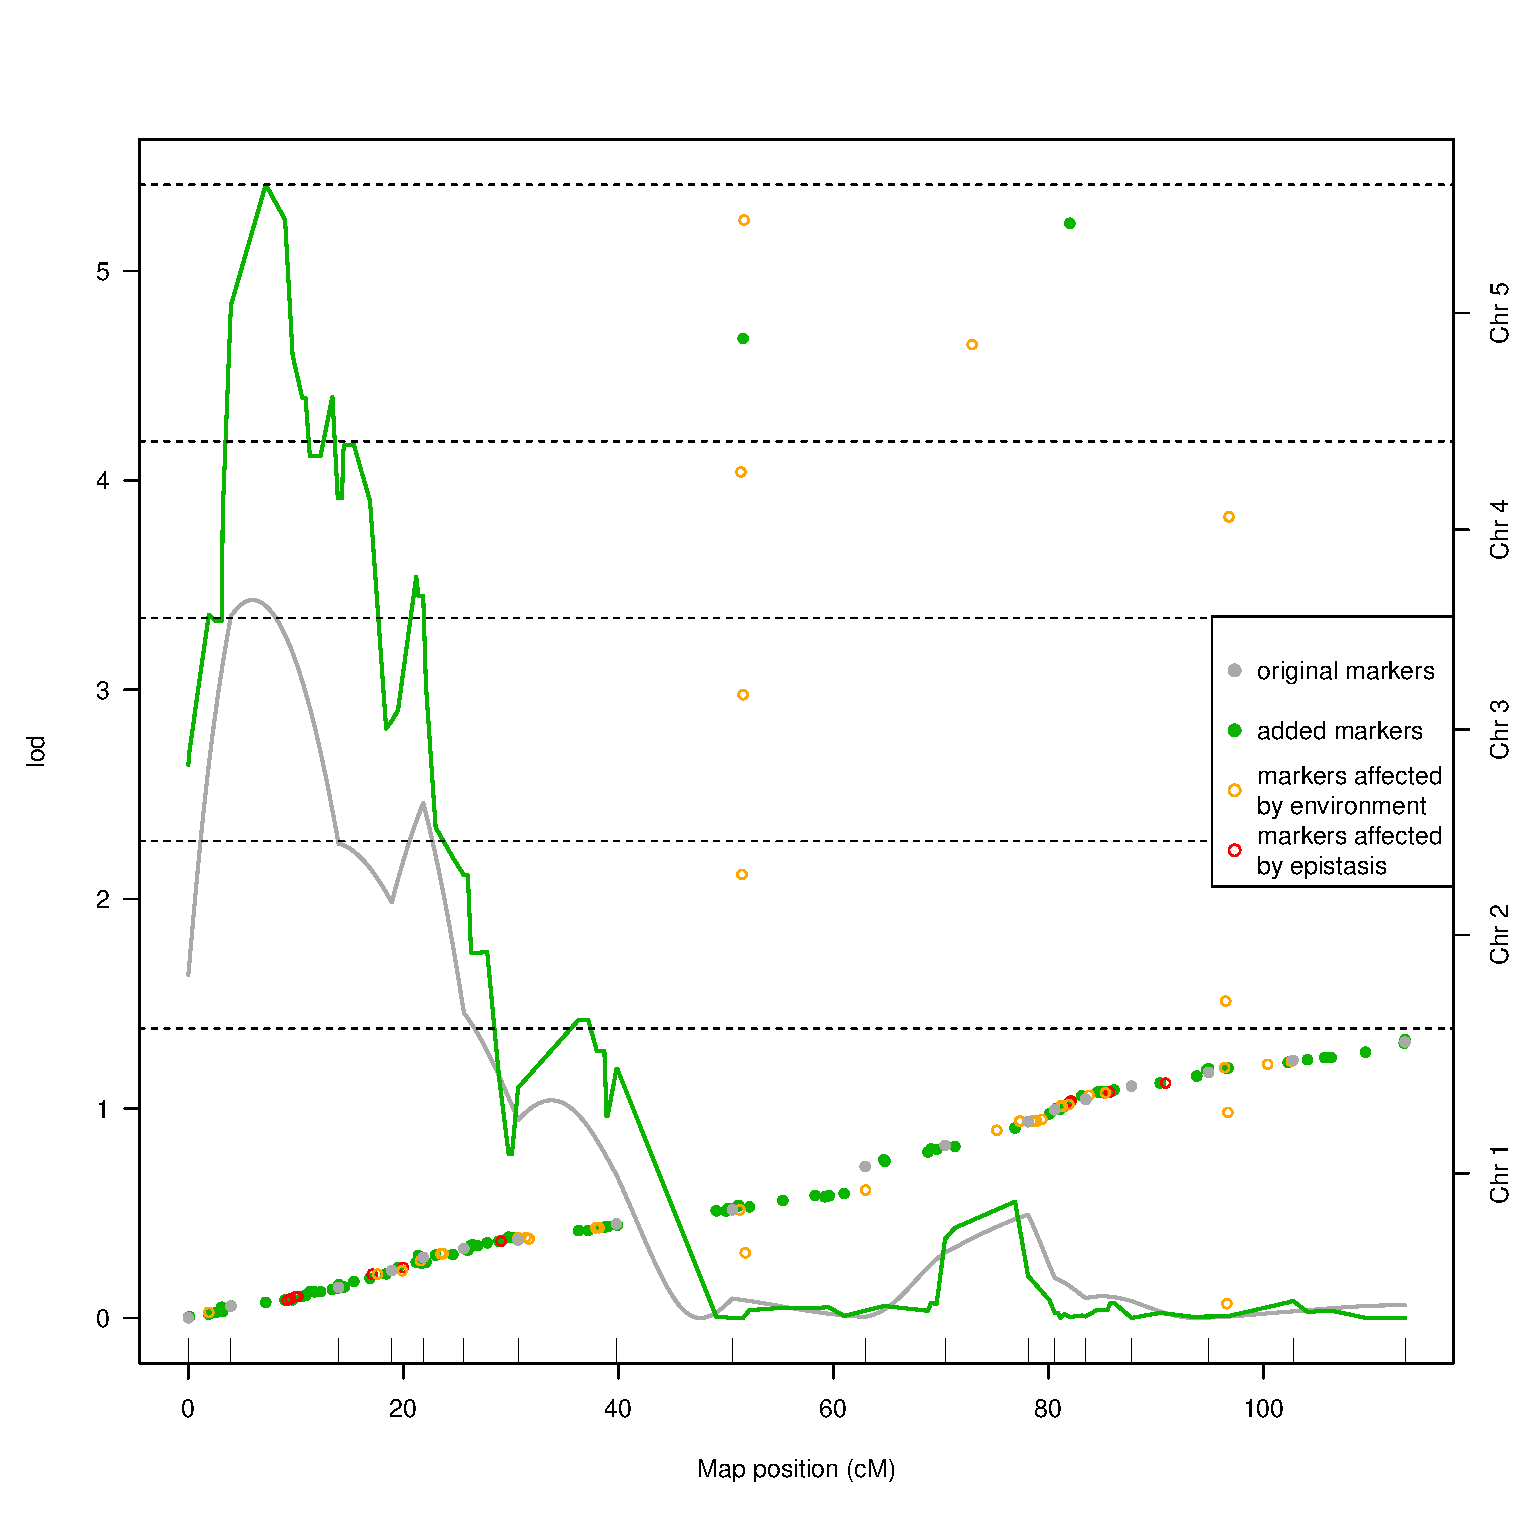
\includegraphics[keepaspectratio,width=0.8\textwidth]{eps/image_2_2.eps}
  \caption[single-marker QTL mapping]{Results of single-marker QTL mapping of a classical phenotype on original (gray line) and saturated map (green line)(left axis). 
          Only chromosome 1 is shown.
          {\bf Ticks on an X-axis} - positions of the original markers on the genetic map. 
          {\bf Gray dots} - positions of the original markers on the physical map. 
          {\bf Colored dots and circles} - candidate markers detected by Pheno2Geno.
          {\bf Orange circles} - candidate markers removed because they showed significant environmental influence.
          {\bf Red circles} - candidate markers removed because they showed an epistatic interaction with other genetic markers. 
          {\bf Green dots} - markers used for saturation of the original map. 
          The final saturated map consists of all the green and gray dots. Shown here are locations of the new markers on the old map, in 
          this way maps align for better clarity.}
          \label{fig:qtlcomparison}
\end{figure}

\begin{figure}[h!]
  \centering
  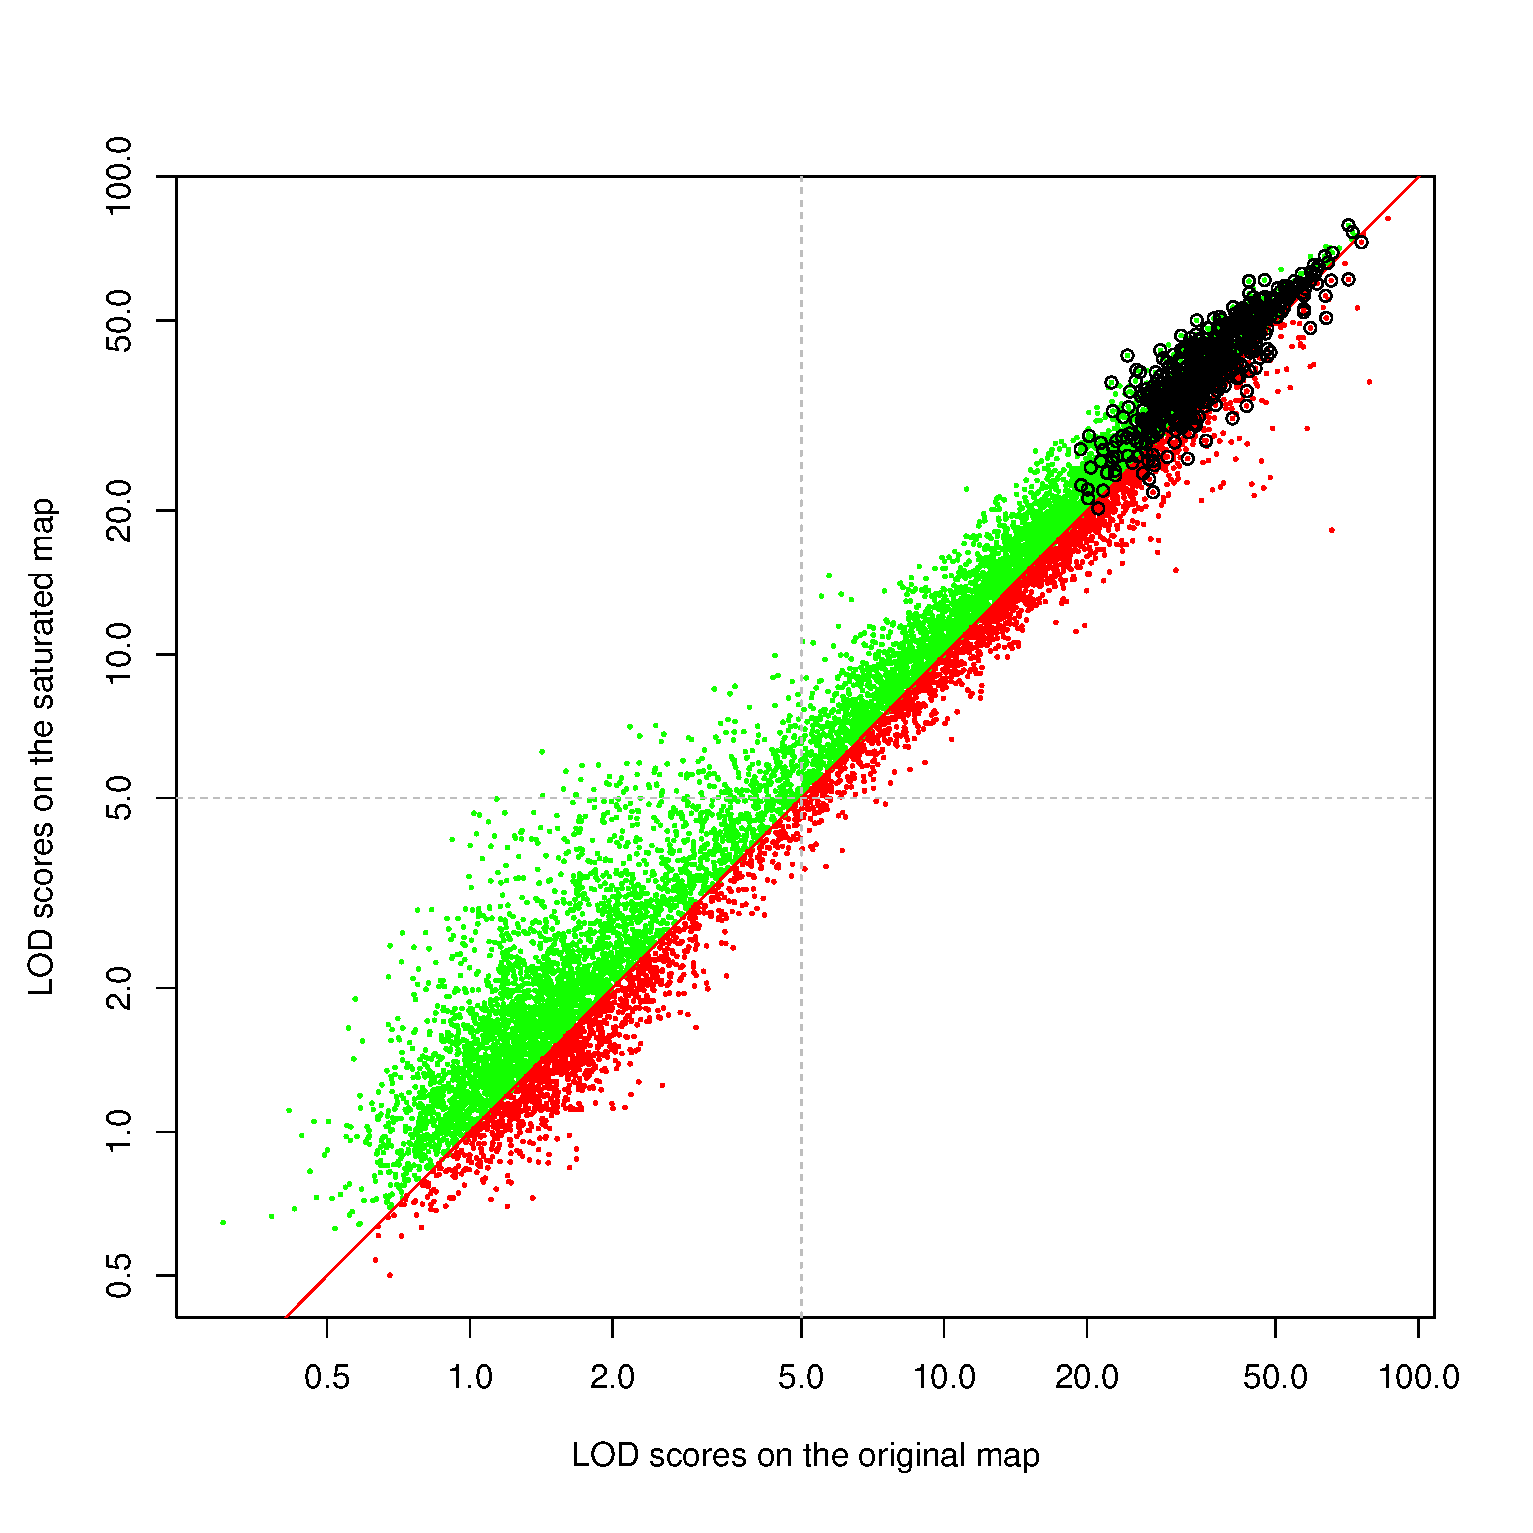
\includegraphics[keepaspectratio,width=0.8\textwidth]{eps/image_2_3.eps}
  \caption[LOD changes.]{
          {\bf A) LOD scores on original and saturated map}. QTL mapping was performed on all 10,801 SNP probes showing differential 
          expression between parents ($p < 0.01$ Student t-test) using original and saturated map. 5837 probes show   a QTL with a 
          $LOD > 5$ on  the original map. {\bf Blue dots} - 3943 probes (66\%) that show an increased LOD score on the new saturated map. 
          Moreover, 210 new QTLs were detected on the saturated map. 
            {\bf Red dots} -  probes showing a decrease in LOD score on the saturated map. 
            {\bf Green circles} - probes used to saturate the map.
          {\bf B) Changing LOD scores.} For each of the phenotypes the top QTL  peak was selected. If the peaks measured on original 
          and saturated map shared location, the differences between LOD scores was calculated. {\bf Solid green line} - median of 
          differences between peaks from chromosome 4, calculated inside a sliding window of 10 cM, moved across chromosome with a 
          step of 1 cM. For each of the windows the value was plotted in the middle of the compartment (hence no value for the first 
          and the last 5 cM). Ticks on the x axis show the position of the markers: {\bf gray tall ticks} - original markers; 
          {\bf green short ticks} - markers selected by Pheno2Geno. Only one region, where no new markers were added (75-80 cM) does not show increase in power. }
  		  \label{fig:qtldetection}
\end{figure}

\section{Features}
Pheno2Geno provides the following functionality to saturate and create genetic maps:

{\bf 1) Preprocessing of the data}: Pheno2Geno offers a selection of 
data transformation functions (including: log, sqrt, reciprocal, probit and logit). 
Gene expression data measured using microarrays are for example generally log 
\cite{Quackenbush:2002} or square root \cite{Jansen:2001a, Gort:2010} transformed before 
further analysis.

{\bf 2) Analysis of parents of segregating population}: When parental data are available 
Pheno2Geno uses a \emph{t}-test to select molecular phenotypes showing significant 
differences between parental strains of segregating population. This reduces the computational load 
of the analysis.

{\bf 3) Analysis of segregating population}:
Phenotypes with a major QTL will show clear multimodal distributions in a segregating 
population. Pheno2Geno fits a mixture model to the phenotype distribution \cite{Jansen:1993, 
Jansen:2001a, Benaglia:2009}. Phenotypes are selected as candidate markers when 
significant multimodality is observed together with mixing proportions close to the expected segregation 
frequency, e.g. 1:1 for a bimodal distribution of two homozygous classes in 
a RIL; 1:2:1 for a trimodal distribution of two homozygous and one heterozygous class in 
an F2 cross.

{\bf 4) Assigning genotypes}:
The posterior probabilities of belonging to an underlying component distribution in the 
mixture is calculated for each component \cite{Jansen:2001b, Benaglia:2009}. Using these 
posterior probabilities, the continuous phenotype values are converted into discrete data 
(e.g. 0 or 1 for RILs; 0, 1 or 2 for F2).  If the posterior probability for a specific 
marker-individual combination is lower than a user-specified threshold, a missing value 
(*) or partly informative value (e.g. not 0, but homozygous 2 or heterozygous 1) is 
assigned to avoid introducing genotyping errors. If parental data is available these can 
be given a parental origin label (A or B for RILs, A, H or B for F2). 
When parental data are not available, mixture-model based scores cannot be converted into 
parental origin labels. Pheno2Geno is able to solve that in case of RILs by forming twice 
as many linkage groups compared to the expected number of chromosomes and then merges 
anti-correlated pairs of linkage groups into a single chromosome.

{\bf 5) \emph{De-novo} construction of genetic maps}: 
When no initial map is available, Pheno2Geno can be used to create an initial 'skeleton' 
map. This skeleton map is produced using very strict settings in the mixture model 
analysis to obtain a limited number of highly trustworthy markers. These candidate markers 
are assigned to linkage groups using the R/qtl function \emph{formLinkageGroups}. 
Additional information provided by the user is used in this step, e.g. known physical 
and genetic positions will be used by Pheno2Geno to assign physical chromosome IDs to 
linkage groups and to determine the correct orientation of chromosomes. The package then 
orders all the markers inside a linkage group by using the R/qtl \emph{orderMarkers} 
function. Finally the skeleton map is saturated to improve resolution as described in 
the next section.

{\bf 6) Environment and epistasis}: 
West et al. \cite{West:2007} emphasized that creation of genetic markers from gene expression data 
is seriously hampered by the presence of environmental variation and multiple possibly interacting 
QTLs (epistasis) suing R/qtl. Pheno2Geno tests if candidate markers are affected by multiple QTLs or pairwise 
interactions. When data were collected in multiple environments potential environmental interactions 
are tested. The user decides whether affected candidate markers are flagged or removed from further analysis.

{\bf 7) Saturation of a known map}:
Pheno2Geno performs interval mapping (using the R/qtl \emph{scanone} function) of 
candidate markers on the original map. The candidate markers are placed on the position 
of the QTL peak. The map is re-estimated (using the R/qtl \emph{est.map} function). 
Followed by  removal of duplicate candidate markers and markers located at the position 
of a known marker.

{\bf 8) Detection of errors}:
After saturation or \emph{de-novo} construction of a genetic map, Pheno2Geno can detect 
and correct genotyping errors (e.g. double recombinations, missing data, semi informative 
markers) using the R/qtl function \emph{fill.geno}. Furthermore, when saturating a known 
map with available genotype data, Pheno2Geno can detect sample mix-ups in the 
original data using R/lineup (which is part of the R/qtl toolset). Users can also use 
external tools such as MixupMapper \cite{Westra:2011} beforehand to detect and correct the 
original genotype data.

\section{Results}
In order to test our package, we performed an analysis of a population with a sparse map.
The original AFLP map was created using a population of 420 RILs derived from a cross between 
\emph{Arabidopsis thaliana} Bayreuth (Bay-0) x Shahdara (Sha) \cite{Loudet:2002}. 
Our dataset consists of 164 RILs from the core population, which were assigned to 4 conditions 
using the designGG package \cite{Li:2009}. Parents were measured in duplicate per condition. 
Gene expression was measured on 370,000 transcripts. During Quality Control 16 arrays 
(all RILs) were discarded, leaving 148 RILs and 16 parental arrays for further analysis.

The original map contained 69 AFLP markers at an average map distance of 7.1 cM \cite{Loudet:2002}. 
Resolution of a genetic map is limited by the size of the population from which the map is derived. 
A distance of 1 cM is equal to 1 recombination in a 100 individuals. Our sample size of 148 
individuals implies that we can obtain at best a resolution of 0.68 cM between markers.

10,801 phenotypes are detected as being differentially expressed between parents 
($P < 0.01$). Mixture modeling identified 1,230 potential markers showing approximately 1:1 
segregation ratio. Pheno2Geno removed 267 markers which show QTL by environment interaction
($LOD >= 7.5$), and 286 candidate markers which show none ($LOD < 15$) (279 markers) or 
multiple QTL (7 markers). Scanning for epistasis showed 77 candidate markers which appear to 
show pairwise epistatic interactions ($LOD >= 7.5$). 

Using the remaining 600 candidate markers the original map was saturated, and 103 co-localizing 
markers were removed. This resulted in 497 new gene expression based markers (720\% increase). 
ap distances were re-estimated (est.map) using the Kosambi's map function. Map expansion was 
observed on chromosomes 4 and 5 increasing total map length from 480.7 to 501.5 
cM (Fig. \ref{fig:mapcomparison}). Nonetheless, the saturation resulted in decreasing the average map distance 
from 7.1 cM to 0.89 cM. This is close to the theoretical resolution limit (0.68 cM) given 
the size of population. Saturation of the \emph{A. thaliana} Bay-0 x Sha map led to a more 
than sevenfold improvement in marker density at no additional lab cost. 

A \emph{de-novo} reconstruction using gene expression data only (ignoring the original 
markers and map) would have led to a skeleton map containing 227 markers with average 
distance of 2.2 cM. 

Additionally, we performed a QTL mapping of our previously published classical 
phenotype dataset\cite{Joosen:2011} onto the saturated map. This showed an increase in QTL 
likelihood for 56\% of previously detected QTLs. Additionally, 29 new QTLs were detected 
on the saturated map. These QTLs showed LOD scores close to the threshold when mapped 
onto the original map ($ 3.4 <= LOD <= 5$, Fig. \ref{fig:qtlcomparison}).

Finally,  a QTL mapping of all the gene expression probes showing differential expression 
between parents (10,801 probes) was performed. 5,837 probes had a significant ($LOD > 5$) 
QTL on the original map. Out of these, 3,943 probes (66\%) showed an increase in QTL 
likelihood on the saturated map (Fig. \ref{fig:qtldetection}) and additional 210 new significant QTLs are 
detected on the saturated map.
  
\section{Conclusions and Discussion}
Pheno2Geno is a generic software package for generating genetic markers and maps from 
high-throughput molecular phenotypes for any inbred diploid population (e.g: backcross, 
F2 intercross and recombinant inbred lines). Pheno2Geno has four important features which 
we will discuss one by one:

{\bf 1) Big data computation.}
Pheno2geno can process large volumes of different kinds of molecular phenotypes \cite{Trelles:2011}. 
Memory requirements of the algorithm are decreased by reading in and processing 
files in chunks rather than at once. Complete analysis of the showcase data (370,000 transcripts) 
is performed under an hour on an average desktop PC (Intel Core i5, 4 GB of RAM). For even larger 
datasets, the Pheno2Geno package is embedded in xQTL workbench \cite{Arends:2012, Snoek:2012} 
allowing for easy parallelization, use of cluster and cloud computing.

{\bf 2) Integration with R/qtl.}
The package is employing well optimized methods and functions of R/qtl for all the mapping steps,
filling and (re)estimation of maps. Moreover, genetic maps created by Pheno2Geno can be directly 
used in R/qtl, providing a smooth transition from genetic map creation to QTL mapping.

{\bf 3) Strict selection of candidate markers.}
The analysis of Pheno2Geno contains multiple selection steps filtering out candidate markers of 
low quality. E.g. candidate markers affected by multiple QTLs and/or environment are flagged and 
can easily be excluded from the analysis.

{\bf 4) Gene expression phenotypes.}
We have illustrated Pheno2Geno on array-based gene expression data. If a gene expression 
phenotype shows a significant QTL (eQTL) and if this eQTL co-localizes with the probe (a 
local eQTL), then the derived marker will be mapped at the location of the probe. The eQTL 
may actually be caused by polymorphisms in the region targeted by the probe \cite{Alberts:2005, 
Alberts:2007}. If the QTL does not lo-localize with the probe (a distant eQTL), the derived 
marker will not be located at the region targeted by the original probe but correctly at the 
position of the distant eQTL.



\chapter{High throughput (Multiple) QTL mapping}
\thispagestyle{empty}
\label{chap:mqm}

\emph{This chapter describes the implementation of the Multiple QTL mapping (MQM) 
routine into R/qtl. Adding a 'new' algorithm to the R/qtl toolset to provide a wider range of 
QTL mapping tools for inbred crosses. R/qtl allows researchers to analyse data from different 
sources or to quickly compare different approaches. This chapter showcases our contributions 
to the R/qtl package such as: MQM, visualizations, parallel computation of QTLs and an improved 
permutation scheme. We evaluated the performance of MQM on classical phenotypes and metabolite 
abundance in A. thaliana, showing improvement in the number and significance of detected QTL 
compared to mapping using a single marker model. }
\null
\vfill

\begin{myexampleblock}{Originally published as:}
  \authors{Danny Arends*, Pjotr Prins*, Ritsert C. Jansen and Karl W. Broman}\\
  \emph{R/qtl: High throughput Multiple QTL mapping}\\
  \bold{Bioinformatics} 26(23):2990-2 (2010) \\

  \authors{Danny Arends*, Ronny V. L. Joosen*, Leo Willems, Wilco Ligterink, Henk Hilhorst, Ritsert C. Jansen}\\
  Visualizing the genetic landscape of Arabidopsis seed performance\\
  \bold{Plant Physiology} 158(2):570-89 (2011)\\

  \authors{Danny Arends*, Ronny V. L. Joosen*, Yang Li*, Leo Willems, Joost J.B. Keurentjes, Wilco Ligterink, 
  Ritsert C. Jansen, Henk Hilhorst}\\
  Identifying genotype-by-environment interactions in the metabolism of germinating Arabidopsis seeds using 
  Generalized Genetical Genomics\\
  \bold{Plant Physiology} 162(2):553-66 (2013)
\end{myexampleblock}

\newpage

Here we show he contributions made to R/qtl and show the application of our newly developed toolset 
to map genetic variation underlying classical phenotypes in \emph{A. thalaina} seed development. We 
show that by using a reduced number of individuals using the designGG strategy we can map main- and 
interactioneffects with more statistical power compared to other designs. After this we use a limited 
number of individuals and continue our analysis by zooming into the metabolic level, we show that 
there are shared genetic loci between phenotypes at different bio-molecular levels. Additional using 
the new optimized MQM routine allows us to detect more loci and/or give more confidence in the loci 
detected.

\section{Single marker QTL mapping (R/qtl)}
R/qtl is an extensible, interactive environment for the mapping of quantitative trait loci (QTL) 
in experimental crosses. It is implemented as an add-on package for the freely available and 
widely used statistical language/software R \cite{R:2009}. Since its introduction, R/qtl 
\cite{Broman:2003} has become a reference implementation with an extensive guide on QTL mapping 
\cite{RQTLGuide:2009}. R/qtl development is continuous, with input from multiple collaborators 
and users.  We have introduced a full testing environment with regression testing, updated the 
license to the GPL version 3, and hosted the source code repository on Github, which gives R/qtl 
software development high visibility and transparency. 

The development of R/qtl reflects trends in quantitative genetics, in particular the use of 
larger datasets, larger calculations and requirements for controlling the false discovery rate. 
These developments are partly driven by high-throughput genetical genomics the name coined 
for the study of gene expression QTL (eQTL)\cite{Jansen:2001a}, metabolite QTL (mQTL), protein 
QTL (pQTL).

\section{Multiple QTL mapping}
\label{sect:mqm}
Multiple QTL Mapping (MQM) belongs to a family of QTL mapping methods, that include Haley-Knott 
regression \cite{Haley:1992} and composite interval mapping CIM \cite{Zeng:1994}. MQM combines 
the strengths of generalized linear model regression with those of interval mapping 
\cite{Jansen:1993, Jansen:1994b}. 

Recent developments in QTL mapping include Bayesian modeling of multiple QTL e.g. R/qtlbim 
package \cite{Yandell:2007, Banerjee:2008}. Bayesian modeling, however, is computationally 
expensive, and arguably has little additional power when applied to high density maps, and 
(nearly) complete genotype data \cite{Handbook:Jansen:2007}. Still, we intend to combine the 
strengths of the different methods in future versions of R/qtl.

These days, with most experimental setups and high density maps, improving precision may be 
achieved by increasing the population size first. For more information on QTL mapping and 
Bayesian analysis we refer to the `Handbook of Statistical Genetics` \cite{Handbook:2007}. MQM 
makes \rev{use} of generalized linear models, thereby potentially providing unified analysis of 
non-normal traits.

MQM provides a practical, relevant and sensitive approach for mapping QTL in experimental 
populations. The theoretical framework of MQM was introduced and explored by R.C. Jansen 
\cite{Jansen:1994a} and \rev{is} explained in the 'Handbook of Statistical Genetics' 
\rev{chapter 21} \cite{Handbook:Jansen:2007}. MQM has one known commercial implementation \cite{Mapqtl:2002}, 
which has been used effectively in practical research, resulting in hundreds of papers, e.g., 
in mouse, plant, and fish, respectively \cite{DeMooij:2009, Jeuken:2009, Kitano:2009}. Now, 
with MQM for R/qtl, we present the first free and open source implementation of MQM, that is 
multi-platform, scalable and suitable for automated procedures and large datasets.

\subsection{Features}
MQM for R/qtl is an automated three-stage procedure in which, in the first stage, missing 
genotype data is 'augmented'.  In other words, rather than guessing one likely genotype, 
multiple genotypes are modelled with their estimated probabilities. In the second stage, 
important marker cofactors are selected by multiple regression and backward elimination. 
The third stage, a QTL is moved along the chromosomes using these pre-selected markers as 
cofactors (Fig. \ref{fig:comparison}). QTL are interval-mapped using the most informative 
model selected by either maximum likelihood or restricted maximum likelihood. A refined 
and automated procedure for cases with large numbers of marker cofactors is included. 

\begin{figure}[h!]
  \centering
  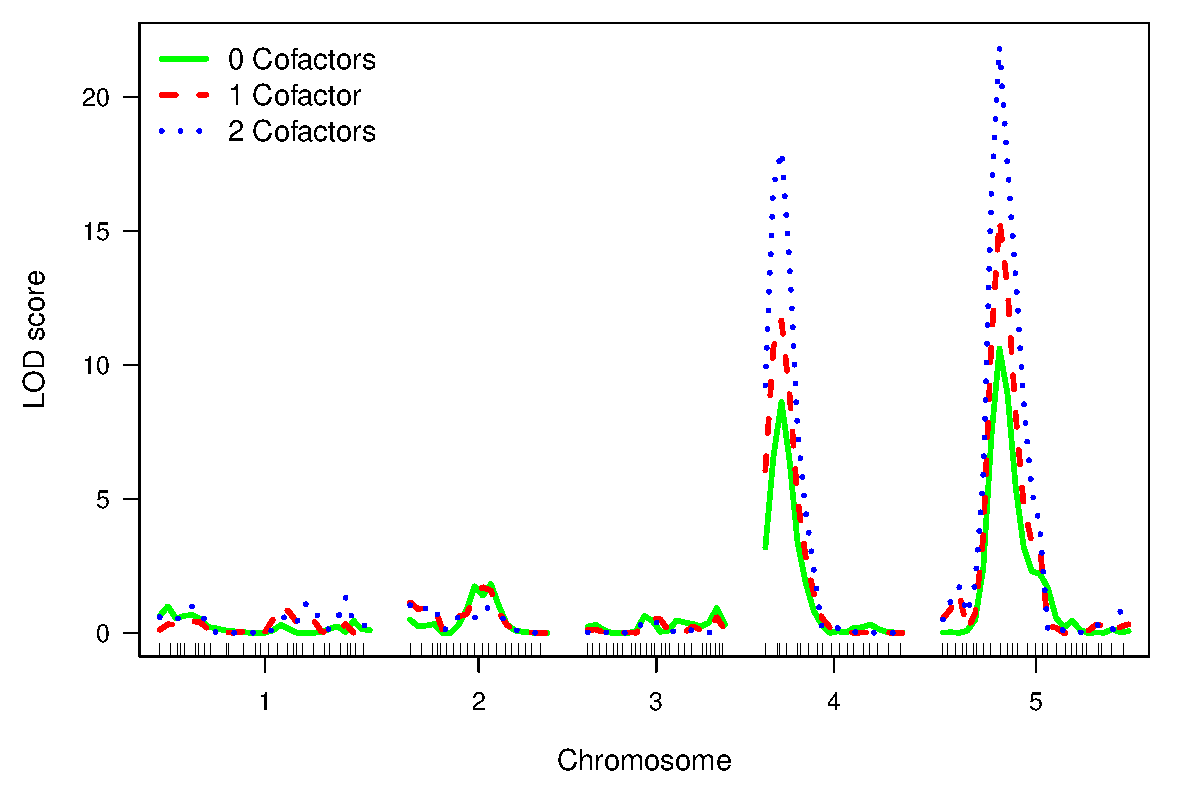
\includegraphics[keepaspectratio,scale=0.30]{eps/image_3_3.eps}
  \caption[Comparison of QTL mapping methodologies.]{ Three way comparison of MQM performance in {\it Arabidopsis 
          thaliana} \citep{Fu:2007}. LOD score increases when cofactors are added manually to the model. Here, 
          adding more than two cofactors does not improve the model any further (as discussed in the online 
          MQM tutorial).}
  \label{fig:comparison}
\end{figure}

The method lets users test different QTL models by elimination of non-significant cofactors. 
MQM for R/qtl brings the following advantages to QTL mapping:
\begin{enumerate}\itemsep1pt
\item Higher power, as long as the QTL explain a reasonable amount of variation.
\item Protection against over-fitting, because MQM fixes the residual variance from the full 
model, which allows the use of more cofactors than may be used in, for example, composite 
interval mapping \cite{Zeng:1994}.
\item Prevention of ghost QTL detection (between two QTL in coupling phase).
\item Detection of negating QTL (QTL in repulsion phase). 
\item MQM gives (compared to CIM) a reduction in type I and type II error \cite{Handbook:Jansen:2007}.
\item A pragmatic permutation strategy for controlling the false discovery rate (FDR) and 
prevention of locating false QTL hot spots, as discussed in Breitling et al \cite{Breitling:2008a}. 
Marker data is permuted, while keeping the correlation structure in the trait data.
\item High-performance computing by scaling on multi-CPU computers, as well as clustered 
computers, by calculating phenotypes in parallel, through the Message Passing Interface (MPI) of 
the SNOW package for R\rev{ }\cite{Tierney:2009}.
\item Visualizations for exploring interactions in a genomic circle plot (Fig. \ref{fig:circleplot}) and \emph{cis}- 
and \emph{trans}-regulation (Fig. \ref{fig:cistrans}).
\end{enumerate}

\begin{figure}[h!]
  \centering
  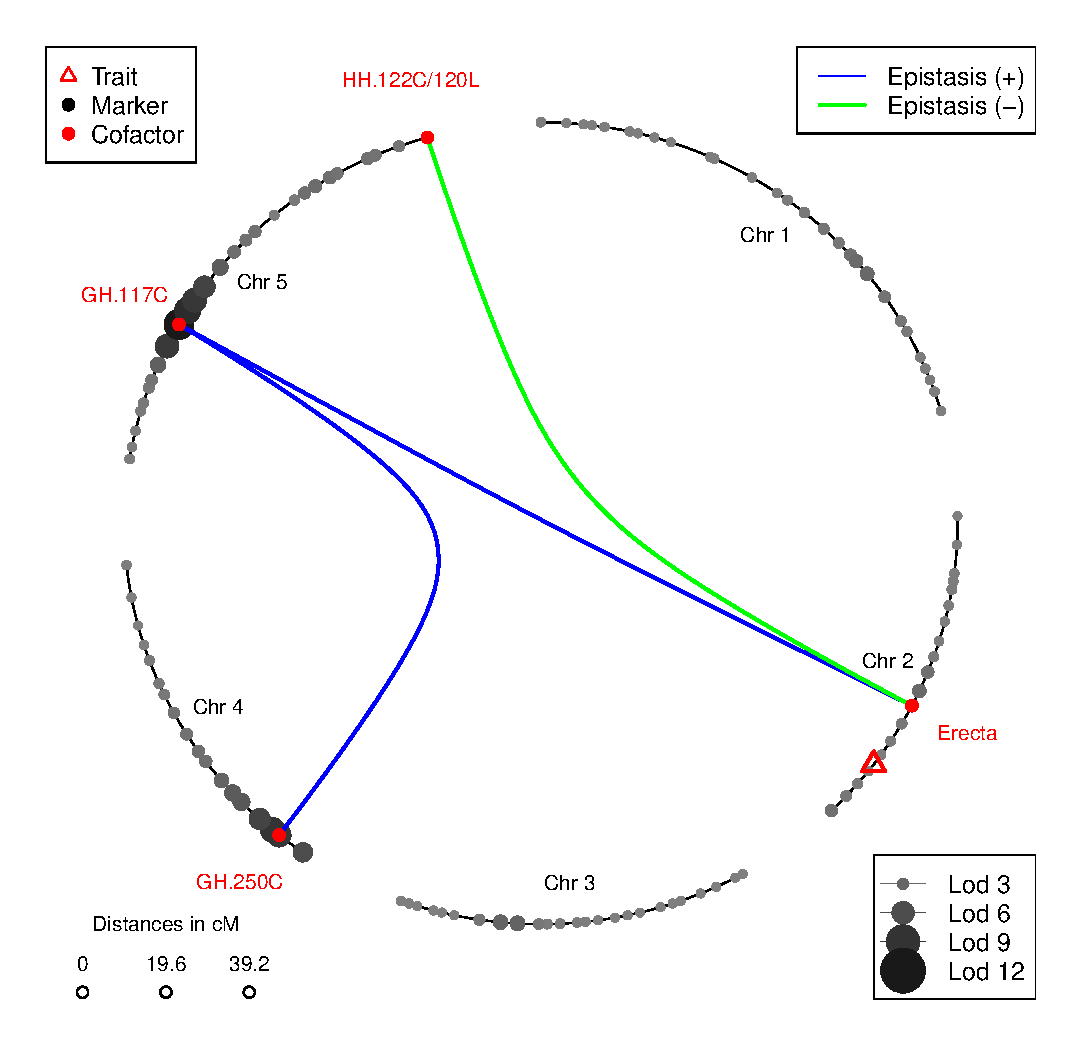
\includegraphics[keepaspectratio,scale=0.30]{eps/image_3_1.eps}
  \caption[Circle plot.]{Circular genome interaction plot \textcolor{black}{of the {\it Arabidopsis 
        thaliana} glucosinolate pathway} \citep{Fu:2007}.  LOD scores shown at marker positions 
        are scaled (grey circles), with selected cofactors (red circles) and epistasis between 
        multiple cofactors (green and blue splines)..}
  \label{fig:circleplot}
\end{figure}

\begin{figure}[h!]
  \centering
  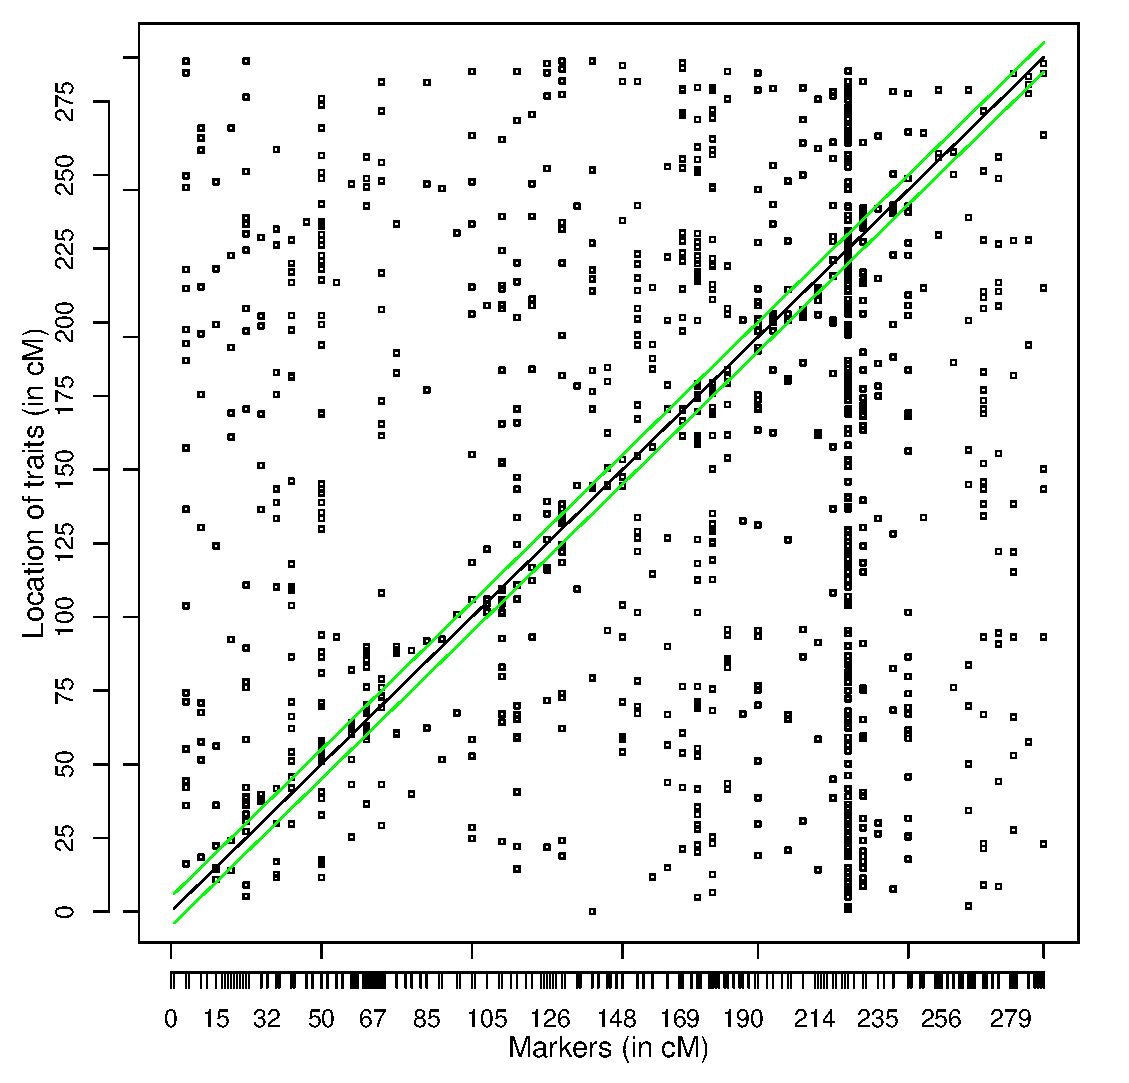
\includegraphics[keepaspectratio,scale=0.30]{eps/image_3_2.eps}
  \caption[CisTrans plot.]{Cis-trans plot of significant QTL (squares) showing cis acting QTL (diagonal) 
          and a trans-band (vertical, chromosome 5) in {\it Caenorhabditis elegans} \citep{Li:2006}.}
  \label{fig:cistrans}
\end{figure}

A 40-page tutorial for MQM explores, both the automated procedure, and the manual procedure 
of adding and removing cofactors, in an \emph{Arabidopsis thaliana} recombinant inbred line 
(RIL) metabolite (mQTL) dataset with 24 metabolites as phenotypes \cite{Fu:2007}. In addition, 
the tutorial visually explains the effects of data augmentation, cofactor selection, model 
selection, and tweaking of input parameters, such as cofactor significance. Genetic interactions 
(epistasis) are explored through effect plots, and an example is given of parallel computation. 
The tutorial is part of the software distribution of R/qtl and is available online.

\subsection{Conclusions and Discussion}
MQM for R/qtl is a significant addition to the QTL mapper's toolbox. R/qtl provides the user 
with the most frequently used statistical analysis methods: single-marker analysis, interval 
mapping, Haley-Knott regression \cite{Haley:1992}, CIM \cite{Zeng:1994} and MQM \cite{Jansen:1994a}. 
MQM has improved handling of missing data and allows more powerful and precise detection of QTL, 
compared to many other methods. Not only is this new implementation of MQM available in the
statistical R environment, which allows scripting for pipe-lined setups, it is also highly 
scalable through parallelisation and paves the way for high-throughput QTL analysis. With MQM, 
R/qtl is a free and high-performance comprehensive QTL mapping toolbox for the analysis of 
experimental populations. R/qtl now includes permutation strategies for determining thresholds 
of significance relevant for QTL and QTL hot spots; the first step towards causal inference and
network analysis.



\section{Mapping classical phenotypes}
Perfect timing of germination is required to encounter optimal conditions for plant survival and it 
is the result of a complex interaction between molecular processes, seed characteristics and 
environmental cues. To detangle these processes we made use of natural genetic variation present in 
an Arabidopsis thaliana Bayreuth x Shahdara RIL population. For a detailed analysis of the germination 
response we characterized rate, uniformity and maximum germination and discussed the added value of 
such precise measurements. The effects of after-ripening, stratification and controlled deterioration 
as well as the effect of salt (NaCl), mannitol, heat, cold and ABA with and without cold stratification 
were analyzed for these germination characteristics. Seed morphology (size, length) of both dry and 
imbibed seeds were quantified by using image analysis. For the overwhelming amount of data produced 
in this study we developed new approaches to perform and visualize high throughput QTL analysis. 
We show correlation of trait data, (shared) QTL positions and epistatic interactions. The detection 
of similar loci for different stresses indicate that often the molecular processes regulating 
environmental responses converge into similar pathways. 7 major QTL hotspots were confirmed using a 
HIF approach. QTLs co-locating with previously reported QTLs and well characterized mutants are 
discussed. A new connection between dormancy, ABA and a cripple mucilage formation due to a natural 
occurring mutation in the MUM2 gene is proposed and this is an interesting lead for further research 
on the regulatory role of ABA in mucilage production and its multiple effects on germination parameters.

\subsection{Background}
Colonizing plants are subject to a wide variety of environmental conditions. For successful adaptation 
to new habitats the timing of developmental transitions is especially important. Seed germination is 
one of these important transitions as it determines the seasonal environment experienced in further 
plant life \cite{Huang:2010}. Natural populations that develop under distinct environmental conditions 
may reveal genetic adaptation, which can be used to disentangle the signaling routes that are involved. 
Seed germination is described by three phases of water uptake. In phase I the seeds imbibes and 
reinitiates metabolic processes followed by a lag phase (phase II). Further water uptake results in 
protrusion of the radicle through the testa and endosperm (phase III). The moment of radicle 
protrusion through the endosperm is considered to be the moment of germination sensu stricto 
\cite{Finch-Savage:2006}. To characterize the genetic variation of germination related traits we 
focused on the effect of the environment that a seed perceives during germination rather than the 
effect of the environment during maternal plant growth, which has been the subject of other 
studies \cite{Dechaine:2009, Elwell:2011}. 

\begin{figure}[h!]
  \centering
  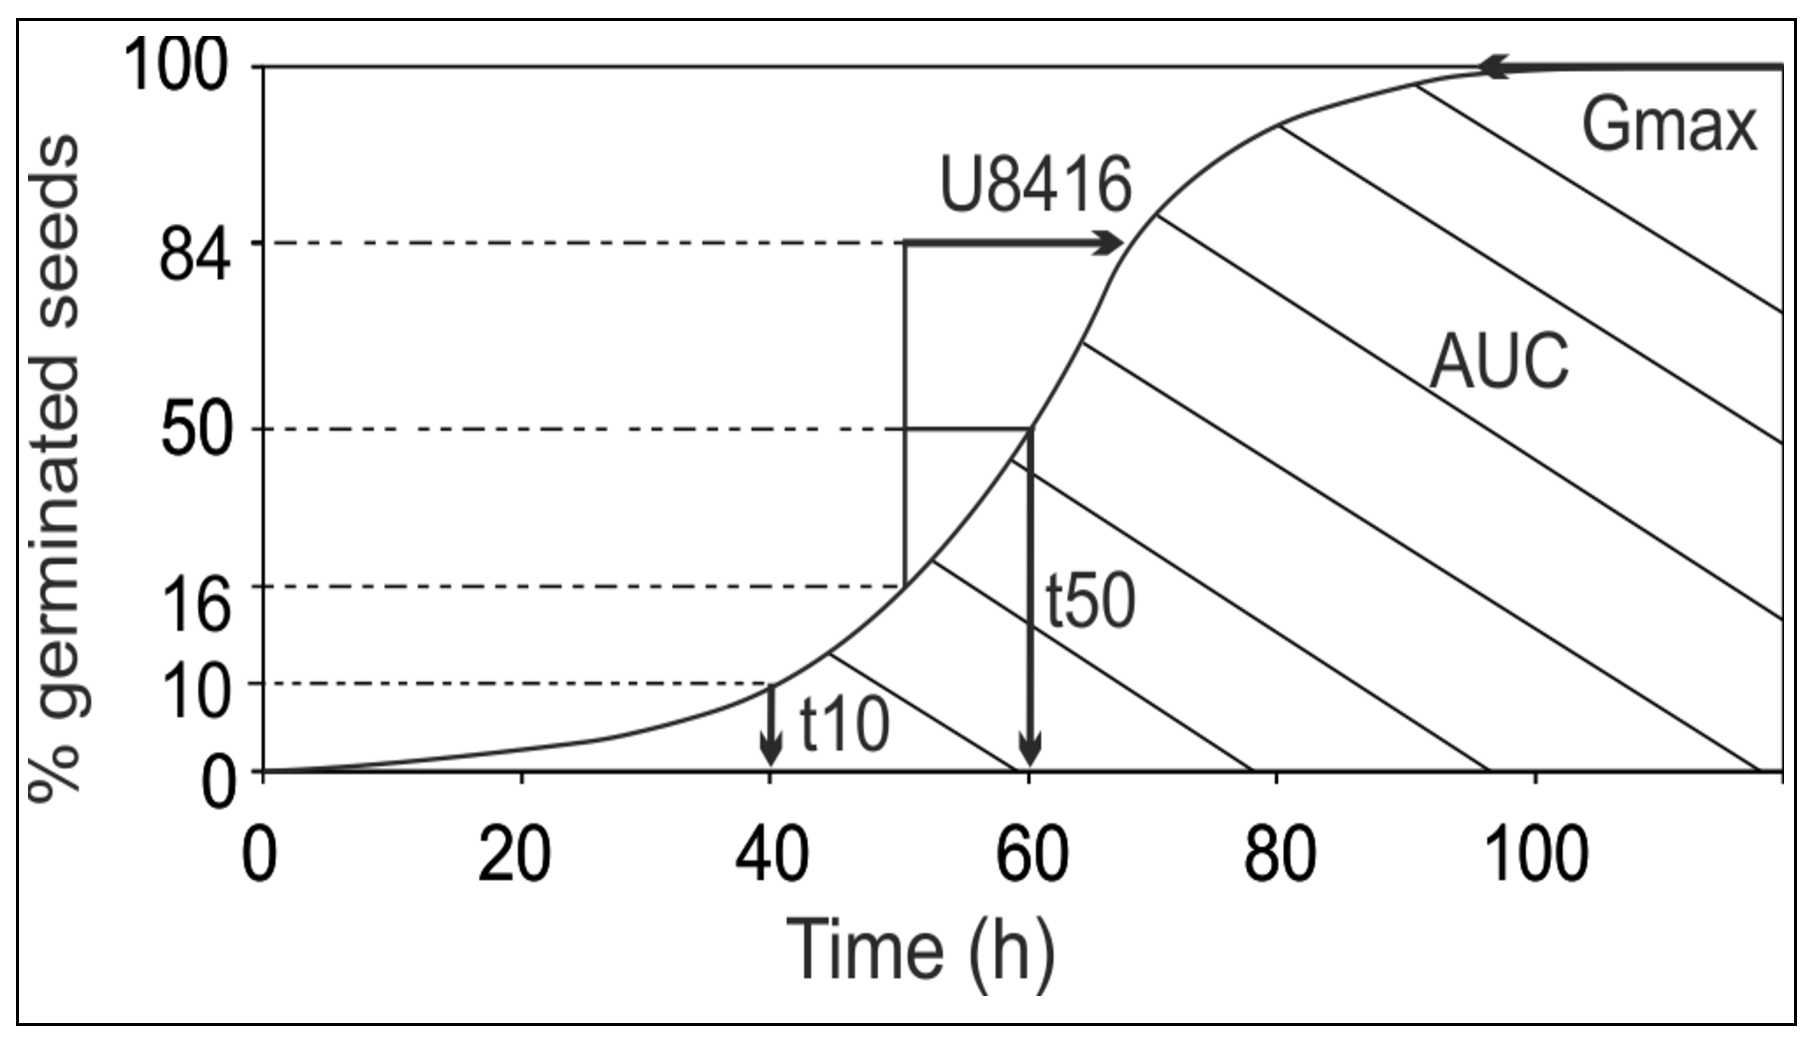
\includegraphics[keepaspectratio,scale=0.30]{eps/image_3_1_1.eps}
  \caption[Germination curve.]
    {Germination curve.}
\end{figure}

Seed content (e.g. oil) is often used as commodity and modifications to the content can therefore be 
regarded as seed quality parameters as well. To prevent confusion we will use the term seed performance 
to indicate that the focus of our study was restricted to seed germination characteristics.

The production of high quality crop seed not only entails knowledge about maternal plant growth, 
harvesting and storage of seeds, but also of germination conditions \cite{Rivero-Lepinckas:2006}. 
To obtain better germination and field performance, many seed companies rely on enhancement methods, 
such as seed priming and coating and/or pelleting, but these methods are reaching their limits. 
Dissecting the molecular mechanisms underlying seed germination and its tolerance to the environment 
may unlock the full genetic potential and enable targeted breeding for seed performance. In this study 
we used a recombinant inbred line (RIL) population derived from two Arabidopsis thaliana ecotypes: 
Bayreuth (Bay-0) which originates from a fallow land habitat in Germany and Shahdara (Sha) which 
grows at high altitude in the Pamiro-Alay mountains in Tadjikistan \cite{Loudet:2002}. The Bay-0 x 
Sha RIL population has been used in many previous studies to map QTL positions for root morphology 
\cite{Loudet:2005, Reymond:2006}, anion content \cite{Loudet:2003a}, nitrogen use efficiency 
\cite{Loudet:2003b}, cell wall digestibility \cite{Barriere:2012}, carbohydrate content 
\cite{Calenge:2006}, sulfate content \cite{Loudet:2007}, leaf senescence \cite{Diaz:2006}, 
morning-specific growth \cite{Loudet:2008} and cold-dark germination \cite{Meng:2008}. We have used 
the natural variation present in this RIL population to map the response of germination characteristics 
to environmental conditions to which a seed is exposed.

\begin{table}[h]
  \centering
  {\footnotesize
  \begin{tabular}{  l  l  l  l  l  l }
    \hline
    {\bf Trait} & {\bf Gmax} & {\bf AUC} & {\bf T50}& {\bf T10}& {\bf A8416}\\
    \hline
    AR.NS           & 0.82 & 0.97 & 0.86 & 0.79 & 0.82 \\
    AR.NS.Cold      & 0.51 & 0.77 & 0.73 & 0.66 & 0.48 \\
    AR.NS.Mannitol  & 0.61 & 0.79 & 0.70 & 0.55 & 0.62 \\
    AR.NS.NACL      & 0.90 & 0.94 & 0.80 & 0.76 & 0.43 \\
    AR.WS           & 0.63 & 0.19 & 0.78 & 0.72 & 0.72 \\
    AR.WS.NACL      & 0.91 & 0.93 & 0.86 & 0.78 & 0.70 \\
    Fresh.NS        & 0.92 & 0.94 & 0.81 & 0.70 & 0.76 \\
    Fresh.WS        & 0.40 & 0.81 & 0.87 & 0.84 & 0.76 \\
    \hline
  \end{tabular}
  }
  \caption[Heritability Overview]{Overview of the broad sense heritability scores. Included are those traits for which different blocks 
          were tested (Trait code descriptions can be found in Table \ref{table:codes})}
\end{table}

Freshly harvested viable Arabidopsis seeds often don't germinate even when placed under conditions 
favorable for germination. This event, called primary dormancy, is shown to be subject to natural 
variation \cite{Bentsink:2010}. In many Arabidopsis ecotypes, this primary dormancy is released after 
a period of dry storage at room temperature. Another dormancy breaking treatment is cold stratification 
were seeds are imbibed in water and stored at 4\degree C in the dark for four days before putting them into 
optimal conditions for germination \cite{Finch-Savage:2006}. Unfavorable conditions during seed 
germination may result in a changed rate or even failure of germination. In Arabidopsis, it has been 
shown that the responsiveness to temperature is closely related to the level of after-ripening 
\cite{Tamura:2006}. High salt concentrations induce osmotic stress and ion toxicity resulting in both 
a delay and reduction of maximum germination \cite{Galpaz:2010}. Often, these different environmental 
stresses are interconnected and will cause osmotic and associated oxidative stress \cite{Zhu:2002, 
Chinnusamy:2004}. The plant hormone Abscisic Acid (ABA) plays a predominant role in plant 
responses to different environmental stresses and can activate various signal transduction pathways 
leading to a global change in transcription \cite{Finkelstein:2002, Xiong:2002}. Exogenous application 
of ABA during germination results in a distinction between testa and endosperm rupture. At certain 
concentrations the testa will rupture but germination sensu stricto (radicle protrusion through the 
endosperm) will be inhibited. This phenomenon, caused by reduced weakening of the endosperm cap, is 
the consequence of a complex interplay between ABA, GA and ethylene signals \cite{Linkies:2009}. 
In this report, we determined germination sensu stricto for primary dormancy in freshly harvested seeds, 
germination of fully after- ripened seeds with and without a preceding cold stratification period 
(see material and methods for conditions), and germination under various stress conditions (low/high 
temperature, salt/osmotic stress and ABA) to assess natural  variation in the Bay-0 x Sha RIL population. 
Additionally, seed morphology (size and length) and flowering time were phenotyped as they have been 
shown to be strong determinants of plant trait variation \cite{Elwell:2011, Chiang:2009, Orsi:2009}. 
We correlated these traits to our germination related traits to evaluate 
possible causality. In total this analysis resulted in 327 trait scores over different harvests. 
Evaluation of these high numbers of phenotypes demanded methods of QTL analysis that extended beyond 
mapping of individual traits and that allowed comprehensive and comprehensible visualization.

\definecolor{C1}{HTML}{2800FF}
\definecolor{C2}{HTML}{8CB4E1}
\definecolor{C3}{HTML}{B4DCE1}
\definecolor{C4}{HTML}{5096B4}

\definecolor{C5}{HTML}{F0F0A0}
\definecolor{C6}{HTML}{FFFF64}

\definecolor{C7}{HTML}{E6DCF0}
\definecolor{C8}{HTML}{B4A0C8}

\definecolor{C9}{HTML}{D2E6B4}
\definecolor{C10}{HTML}{78B478}
\definecolor{C11}{HTML}{78963C}

\definecolor{C12}{HTML}{FAE6DC}
\definecolor{C13}{HTML}{FABE8C}
\definecolor{C14}{HTML}{FA8C32}

\definecolor{C15}{HTML}{DCDCC8}
\definecolor{C16}{HTML}{C8BE96}

\definecolor{C17}{HTML}{E6B4B4}
\definecolor{C18}{HTML}{DC9696}

\definecolor{C19}{HTML}{96FF96}
\definecolor{C20}{HTML}{96C800}
\definecolor{C21}{HTML}{C8C800}

\begin{table}[h]
  \tiny
  \centering
  \begin{tabular}{ | l | c | l | l | p{4cm} | l | }
    \hline
    {\bf Trait Group}    & {\bf Stratification} & & {\bf Harvest} & {\bf Description}                                                                                          & {\bf Codes}               \\
    \hline
    Germination               & N & \cellcolor{C1} & ABCD          & After ripened seed germination                                                                                           & AR.NS                     \\
    \hline
    After ripening            & N & \cellcolor{C2} & ABCD          & Delta between freshly harvested seed germination and after-ripened seed germination                                      & AR.NS - Fresh.NS          \\
    \hline
    Fresh                     & Y & \cellcolor{C3} & ABCD          & Delta between freshly harvested seed germination and freshly harvested seed germination                                  & Fresh.WS -Fresh.NS        \\
    \hline
    AR                        & Y & \cellcolor{C4} & ABCD          & Delta between after-ripened seed germination and after-ripened  seed germination                                         & AR.WS - AR.NS             \\
    \hline
    NaCl                      & N & \cellcolor{C5} & ABCD          & Delta between after-ripened seed germination on 100 mM NaCl and after-ripened  seed germination on water                 & AR.NS - NaCl.             \\
    NaCl                      & Y & \cellcolor{C6} & ABCD          &                                                                                                                          & AR.WS - NaCl.WS.          \\
    \hline
    Mannitol                  & N & \cellcolor{C7} & AD            & Delta between after-ripened seed germination on -0.5 mP Mannitol and after-ripened seed germination on water             & AR.NS - AR.Mann.NS.       \\
    Mannitol                  & Y & \cellcolor{C8} & AD            &                                                                                                                          & AR.WS - AR.Mann.WS.       \\
    \hline
    Cold Fresh                & N & \cellcolor{C9} & D             & Delta between freshly harvested seed germination at 10\degree C and freshly harvested seed germination at 20\degree C    & Fresh.NS - Fresh.Cold.NS  \\
    Cold                      & N & \cellcolor{C10} & AD            & Delta between after-ripened seed germination at 10\degree C and after-ripened seed germination at 20\degree C            & AR.NS - AR.Cold.NS        \\
    Cold                      & Y & \cellcolor{C11} & D             &                                                                                                                          & AR.WS - AR.Cold.WS        \\
    \hline
    Heat Fresh                & N & \cellcolor{C12} & D             & Delta between freshly harvested seed germination at 30\degree C and after-ripened seed germination at 20\degree C        & Fresh.NS - Fresh.Heat.NS  \\
    Heat                      & N & \cellcolor{C13} & D             & Delta between after-ripened seed germination at 30\degree C and after ripened seed germination at 20\degree C            & AR.NS - AR.Heat.NS        \\
    Heat                      & Y & \cellcolor{C14} & D             &                                                                                                                          & AR.WS - AR.Heat.WS        \\
    \hline
    CD*                       & N & \cellcolor{C15} & D             & Delta between after-ripened seed germination after controlled detoriation and after-ripened seed germination on water    & AR.NS - AR.CD.NS          \\
    CD*                       & Y & \cellcolor{C16} & D             &                                                                                                                          & AR.WS - AR.CD.WS          \\
    \hline
    ABA                       & N & \cellcolor{C17}  & D             & Delta between after-ripened seed germination with  0.5 $\mu$M ABA and after-ripened seed germination on water            & AR.NS - AR.ABA.NS         \\
    ABA                       & Y & \cellcolor{C18}  & D             &                                                                                                                          & AR.WS - AR.ABA.WS         \\
    \hline
    Seed size                 & N & \cellcolor{C19} & ABD           & Seed size and length of dry seeds                                                                                        & Size.Area                 \\
    Seed size, imbibed        & N & \cellcolor{C20} & ABD           & Seed size of imbibed seeds                                                                                               & Size.imbibed              \\
    Flowering time            & N & \cellcolor{C21} & ABD           & First open flower in long day (16D/8N) conditions                                                                        & FTLD                      \\
    \hline
  \end{tabular}
  \caption[Trait codes]{Overview of traits in this study and the harvest(s) used for the measurement. The indicated color-code 
          is used in all figures throughout this paper. For each mentioned experiment $G_{max}$, AUC, $t_{50}$, $t_{10}$ and $U_{8416}$ were determined.}
  \label{table:codes}
\end{table}

\begin{figure}[h!]
  \centering
  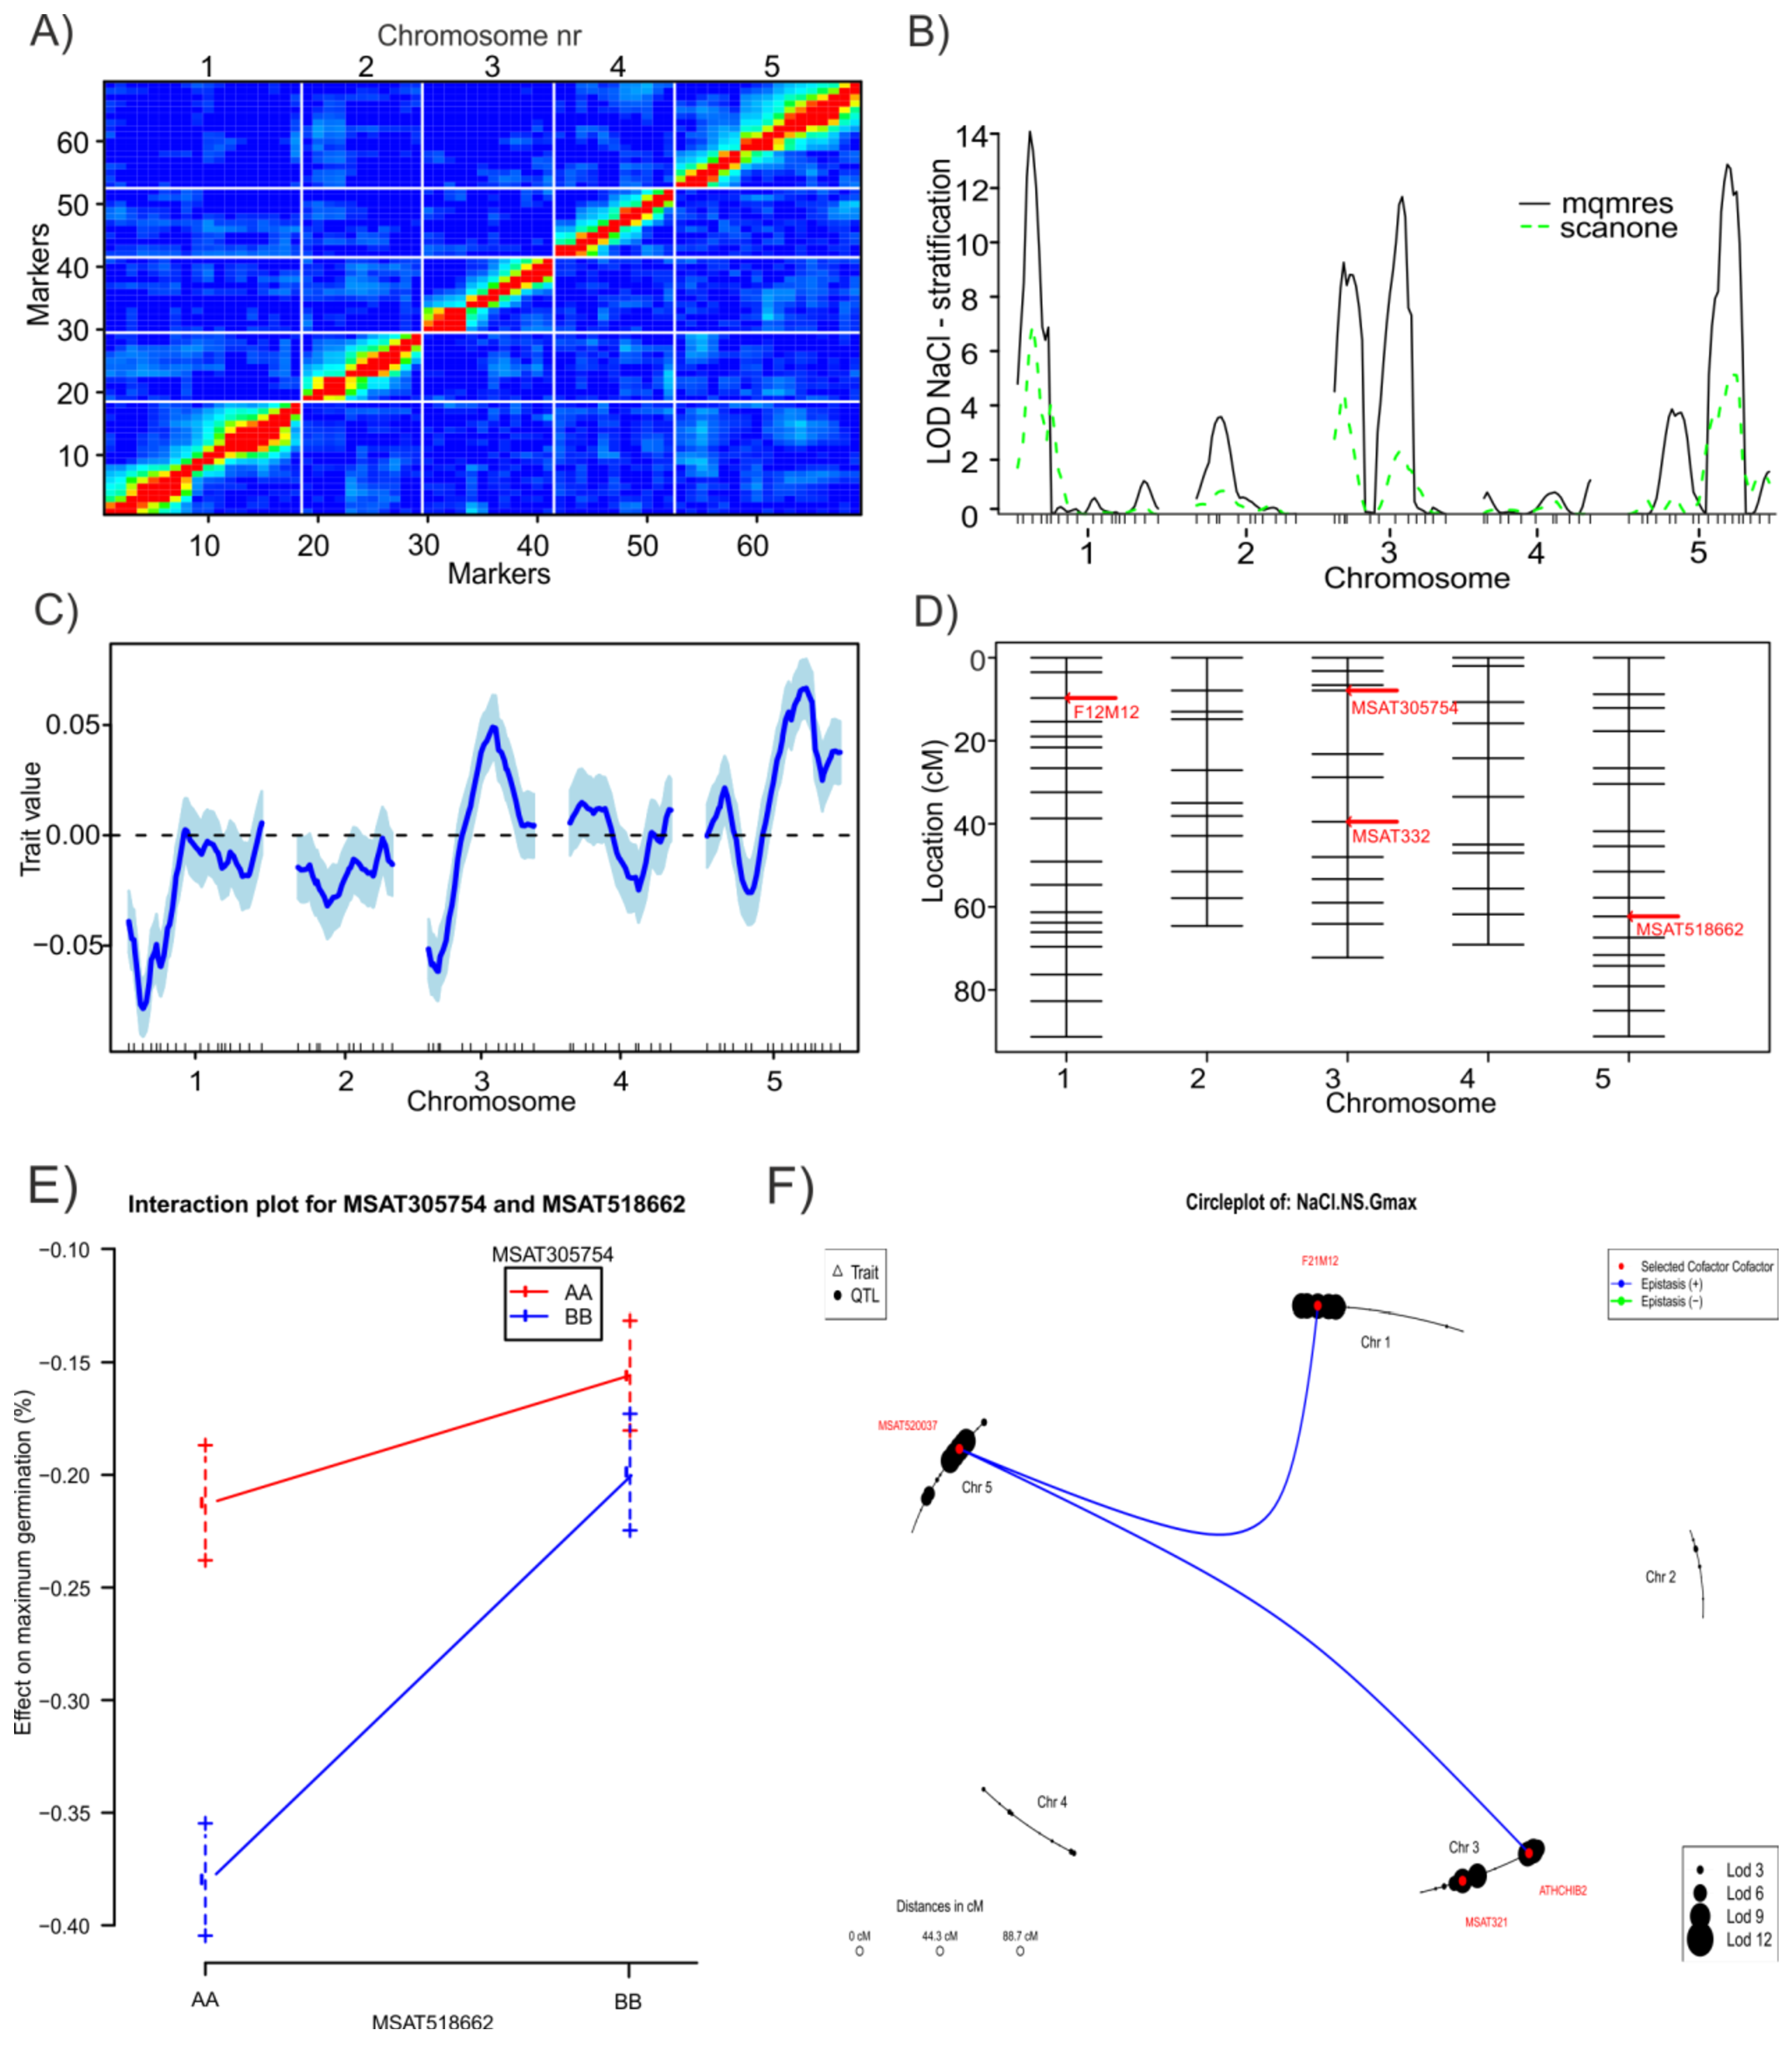
\includegraphics[keepaspectratio,scale=0.30]{eps/image_3_1_2.eps}
  \caption[Generated Output.]{R/QTL output for the effect of 100mM NaCl on the maximum germination without 
          stratification. A) Pairwise recombination fractions; B) Phenotype distribution histogram without 
          normalization ; B) LOD profile comparison between MQM and Haley-Knott (scan-one) interval mapping; 
          C) Genome wide additive effect based on raw phenotype data D) Genetic map showing the significant 
          QTL markers; E) Interaction plot showing the effect size comparison between marker MSAT305754 and 
          MSAT518662 at the Sha (AA) and Bay-0 (BB) alleles; F) Circle plot showing interactions between 
          all significant markers.}
          \label{fig:generatedoutput}
\end{figure}

Analysis of natural variation that is captured in well-defined recombinant inbred populations has 
shown to be a powerful tool to detect important loci that influence the traits under study 
\cite{Alonso-Blanco:2009}. To uncover the loci with genetic variation a statistical framework is 
needed. For this, any programming language can be used which supports statistics. In the life sciences 
the statistical language R is often the prime candidate. R is open source, contains the latest in 
statistical analysis methods and has a large community for help and support (http://www.r-project.org/). 
Furthermore, it has the R/qtl package \cite{Broman:2003}, which contains an array of different 
QTL mapping methods, including Single Marker Mapping, Interval Mapping and Multiple QTL Mapping (MQM) 
\cite{Arends:2010}. Although all possibilities to perform a detailed QTL analysis including data 
preprocessing and output formatting are present in R, it requires extensive knowledge of the R-syntax 
to combine all necessary steps in a single analysis protocol that can loop through hundreds or 
thousands of traits. 

We present a script that can perform these tasks. This type of automated analysis combined with 
efficient data visualization is a necessary step to keep up with the increasing rate of biological 
data production. For using single trait mapping the effect of a certain treatment, e.g. germination 
at high temperature, must be corrected by the germination characteristics under control conditions. 
Here, we subtracted the observed germination under stress conditions from values for germination 
under control conditions. This correction can lead to complicated interpretation, especially when the 
environment under study affects loci with already strong effects under control conditions. Further, 
it can reduce statistical power due to summation of the error components. Therefore we performed an 
additional analysis using a QTL by environment (QTLxE) approach \cite{Vargas:2006, Moreau:2004}. 
Instead of considering individual responses, one can then treat the stress conditions as a set of 
environmental perturbations and evaluate a single trait (such as germination percentage). Because 
several environments are taken into account simultaneously, the statistical power to detect loci 
that are affected by several environments increases and interpretation becomes more intuitive as the 
need for correcting the stress response by the control response is eliminated \cite{Boer:2007}.

The Bay-0 x Sha RIL population consists of 420 lines that were genotyped in the F6. This relatively 
low degree of inbreeding provoked residual heterozygosity present at almost all genome positions. 
This residual heterozygosity can be used to confirm QTL positions, as it provides a possibility to 
study both parental alleles at the locus of interest in an elsewhere homozygous background. 
In contrast to conventional near isogenic lines (NILs) the genetic background of heterogeneous 
inbred lines (HIFs) consist of a mix of the two parental genomes. The availability of a genome wide 
set of HIF lines for the Bay-0 x Sha RIL population provides a fast and accurate means to confirm 
detected QTL loci.

\subsection{Results}

\subsubsection{Single trait QTL mapping}
To evaluate the response of germination to a certain treatment, we first subtracted the observed 
germination at test conditions from germination at the proper control conditions. For example, the 
effect of NaCl on germination after cold stratification is determined by subtracting Gmax on 
NaCl from Gmax on water. This subtraction was reversed for the rate and uniformity parameters to 
correct the reversed nature of these parameters (e.g. slower germination results in a larger t10 
and t50). Table \ref{table:codes} gives an overview of all corrections that have been applied. 

\begin{figure}[h!]
  \centering
  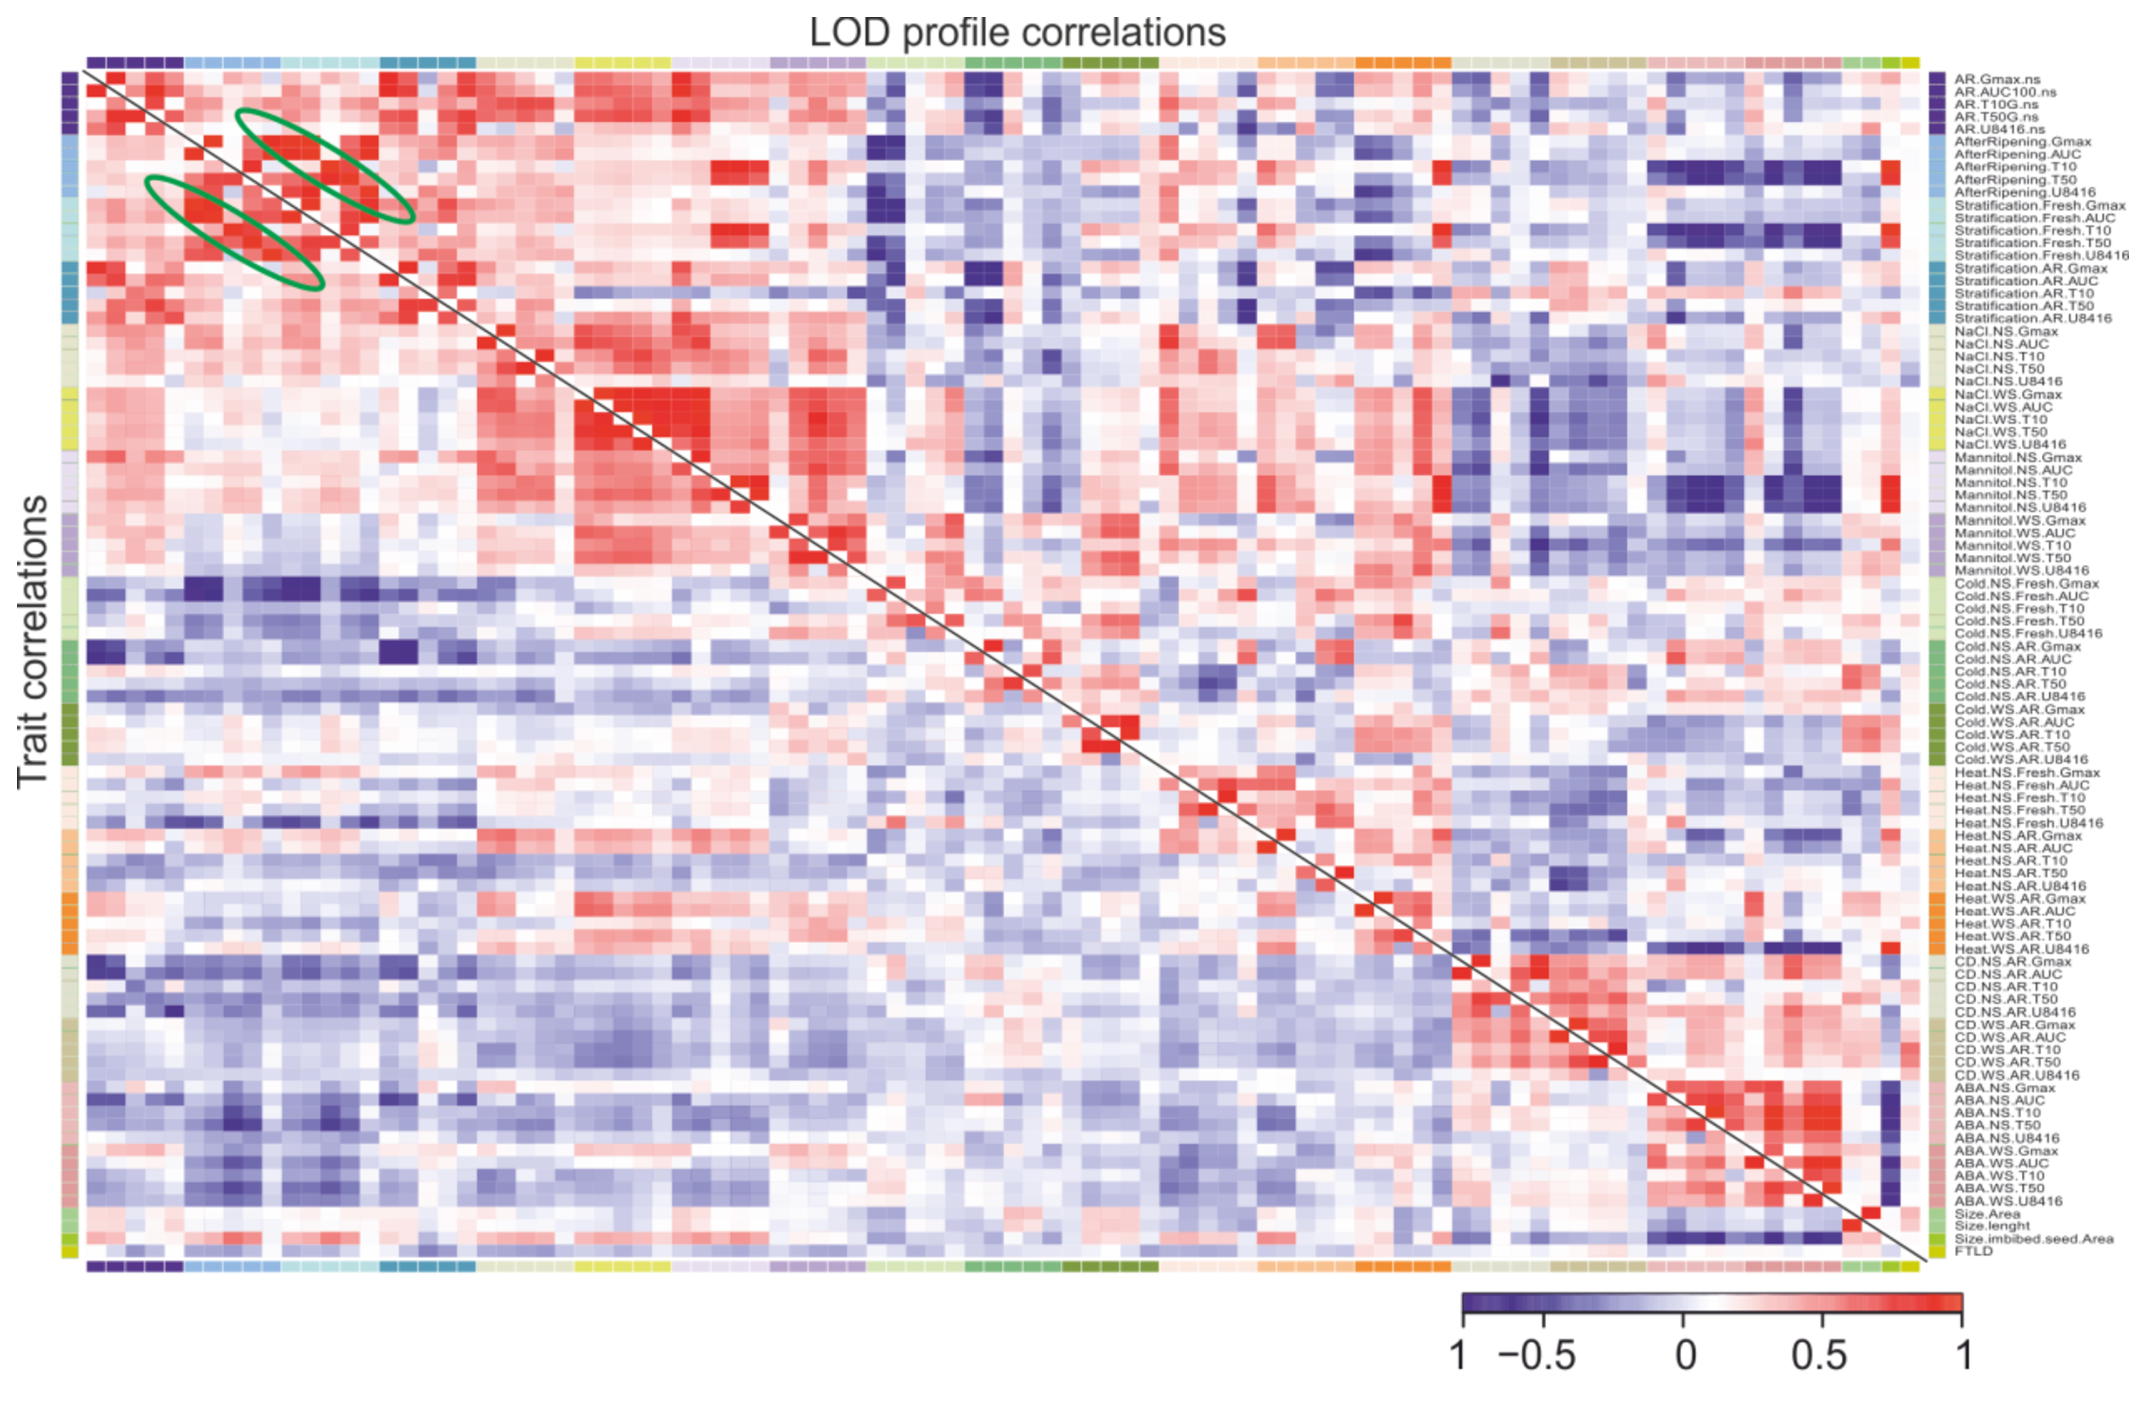
\includegraphics[keepaspectratio,scale=0.30]{eps/image_3_1_3.eps}
  \caption[Heatmap of correlation.]{Correlation between all trait values (bottom left panel) and between 
          all LOD profiles (top right panel). Traits are indicated by the color code depicted in Table \ref{table:codes}. 
          Green circles indicate an example of the close correlation between "after-ripened" and "fresh 
          with stratification" trait values.}
\end{figure}

An analytical protocol was designed, using the popular R/qtl package of R to analyze trait data of 
recombinant inbred populations with the multiple QTL model approach \cite{Arends:2010}. When 
performing a detailed QTL analysis it is important that several steps are performed or checked. 
Missing genotypic data is imputed and a recombination frequency plot is generated (Fig. \ref{fig:generatedoutput}A). In 
the next step, quality of the trait data is investigated. Outliers are detected and removed using 
a Z-score transformation with a user defined threshold. As an extra control the results of MQM mapping 
were always compared to standard interval mapping, using the parametric model with Haley Knott 
regression \cite{Haley:1992} (Fig. \ref{fig:generatedoutput}B). The whole genome additive effect was estimated based 
on the non-transformed data as half the difference between the phenotypic averages for the two 
homozygotes (Fig. \ref{fig:generatedoutput}C).

R/qtl MQM uses a backward elimination of cofactors. As a rule of thumb one can select a maximum of 
$N-20$ initial cofactors with this procedure \cite{Handbook:Jansen:2007}, with $N$ being the number of lines in 
the RIL population. In our script, a cofactor file can be provided with the selection of the initial 
cofactors. When no cofactors are provided, the analysis will be performed without cofactors resulting 
in an analysis comparable with the composite interval mapping (CIM) method. For the analysis of the 
Bay-0 x Sha population we pre-selected 39 out of 69 markers as possible cofactors. Cofactors were selected 
based on their quality (least amount of missing data or heterozygous status) and physical cM position, 
attempting to obtain intervals of about 10 cM. Although the procedure allows the selection of all 69 
markers as cofactors, this does not improve mapping and only lowers statistical power due to the 
multiple testing correction in the permutation analysis. The provided cofactor file is used to perform 
automated backward elimination of cofactors.

\begin{figure}[h!]
  \centering
  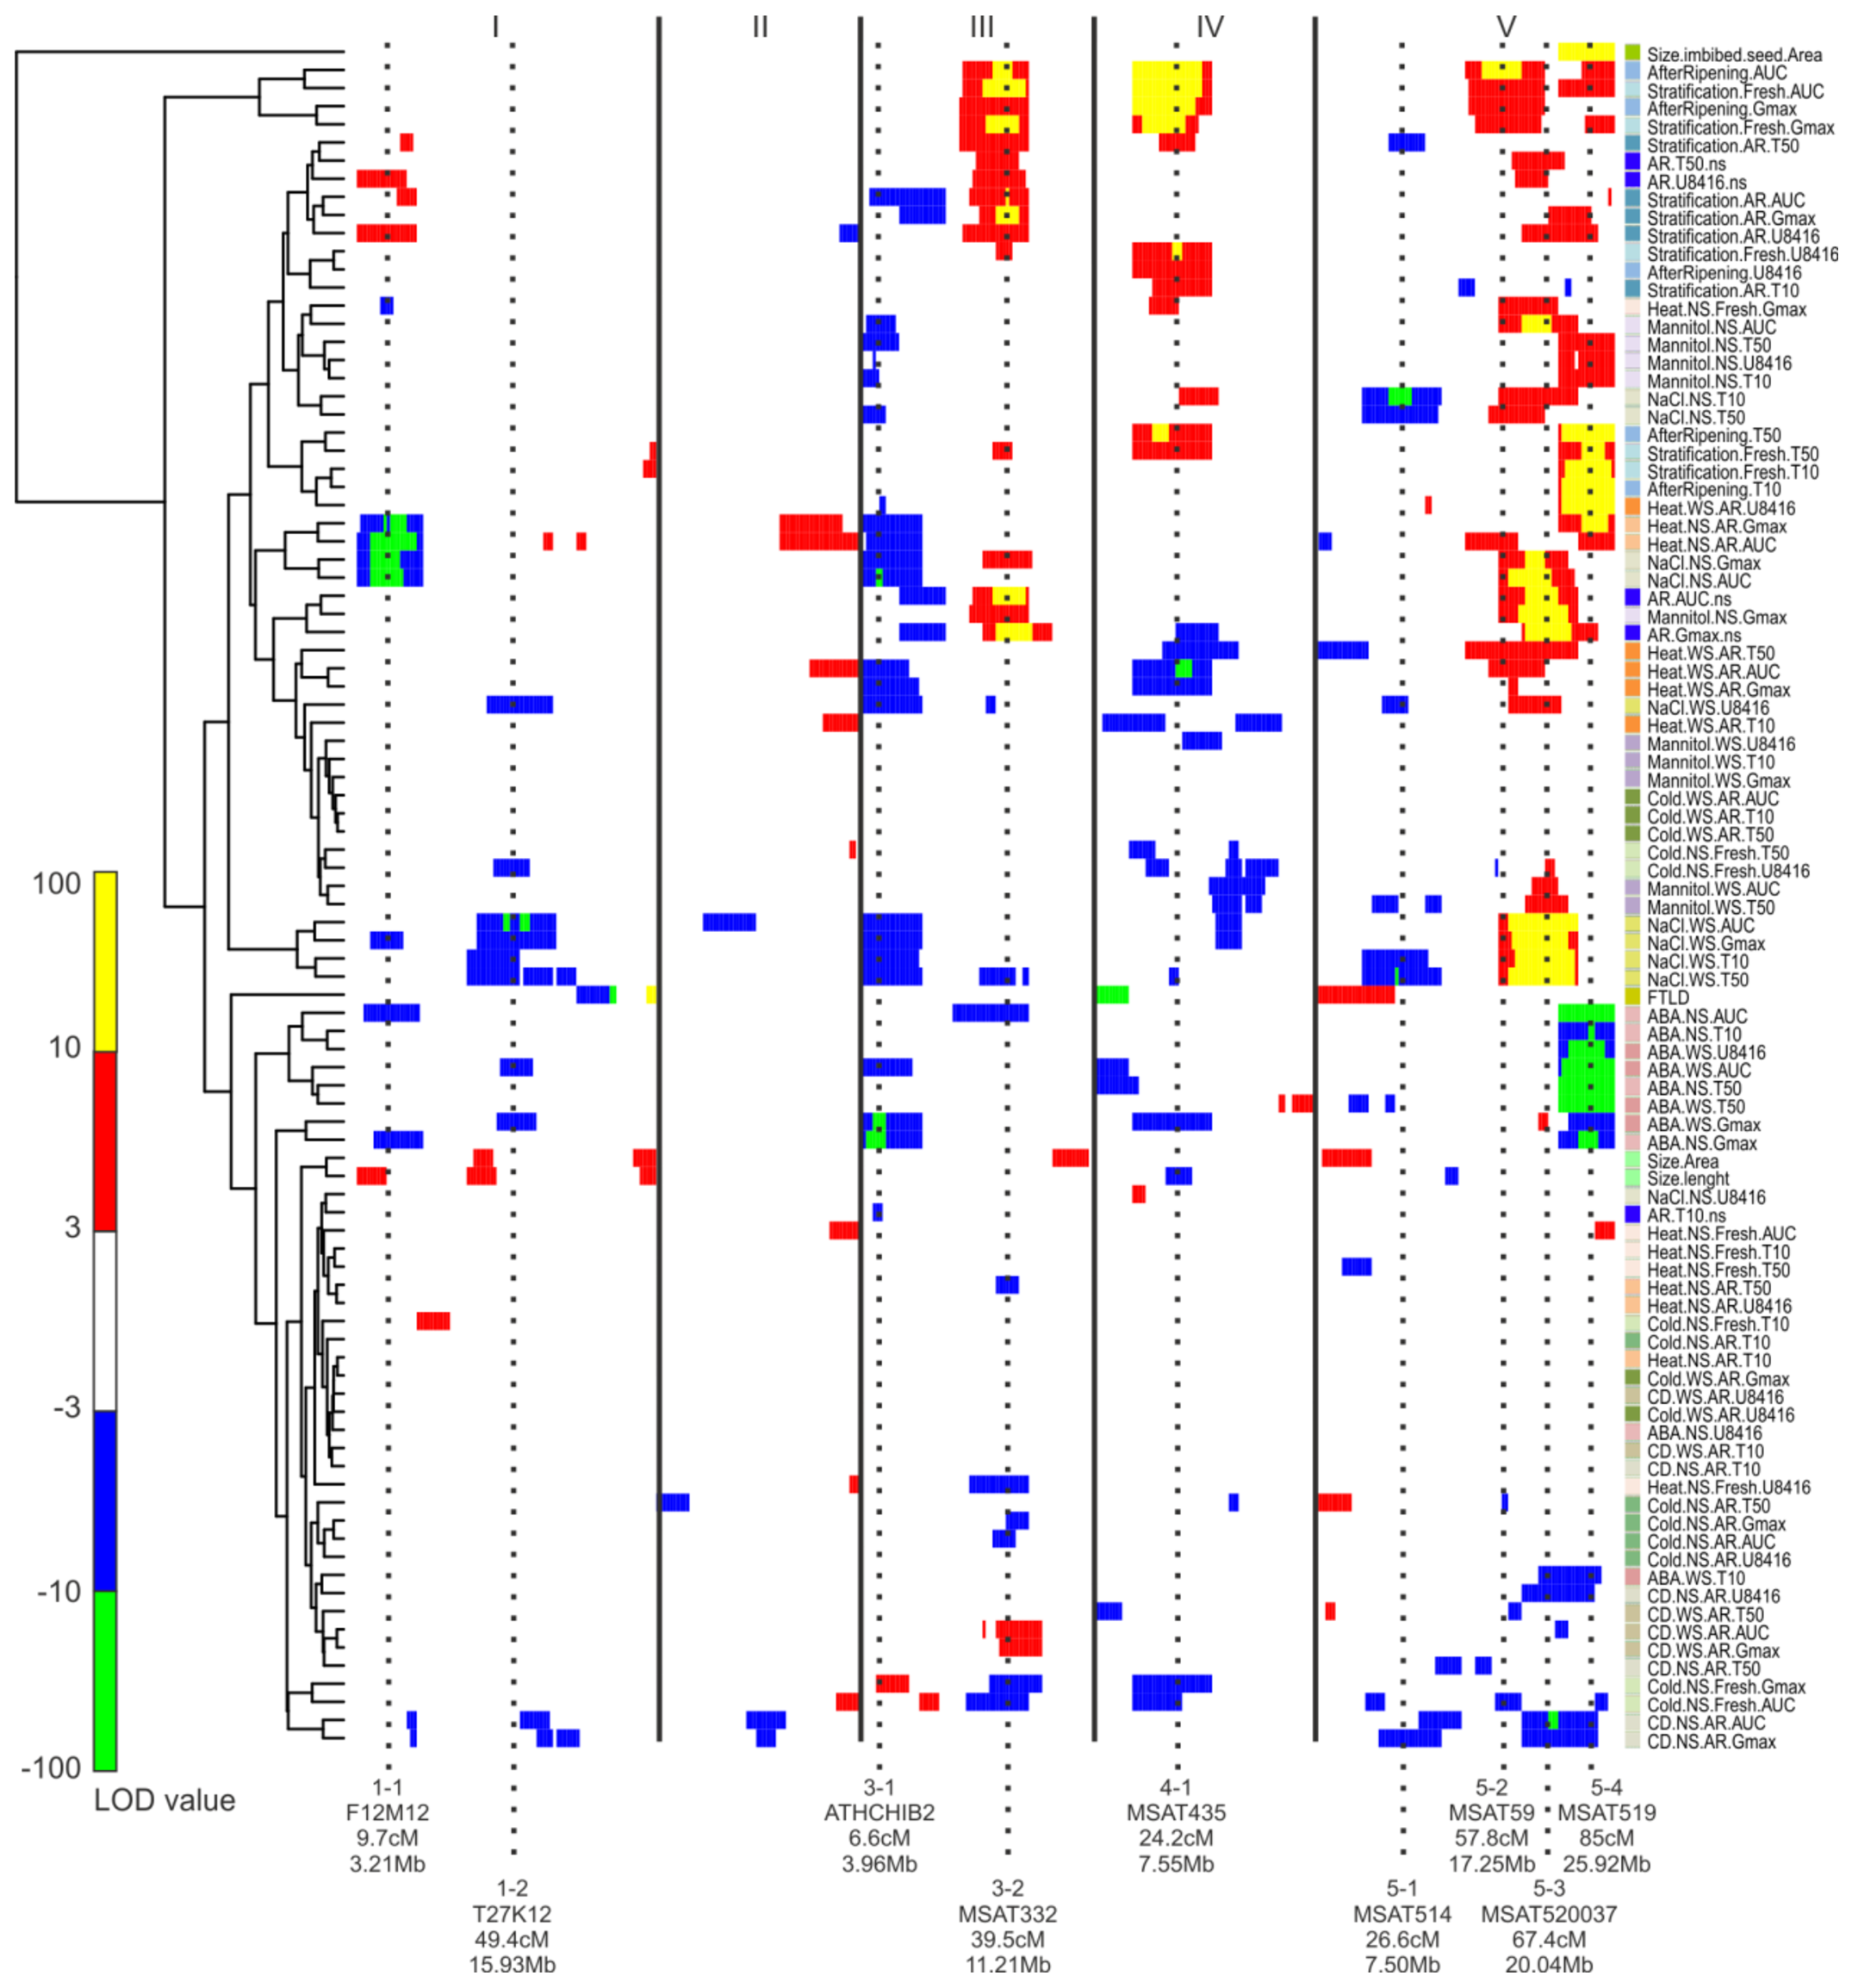
\includegraphics[keepaspectratio,scale=0.30]{eps/image_3_1_4.eps}
  \caption[QTL locations.]{A clustered heat map showing the LOD profiles of the measured traits is automatically 
          produced. Columns indicate chromosome position along the 5 chromosomes; rows indicate individual trait 
          LOD profiles. A false color scale is used to indicate the QTL significance. Positive values (yellow and red) 
          represent a larger effect of the treatment in Shahdara, negative values (blue and green) in Bayreuth..}
\end{figure}

Backward elimination is performed to remove cofactors that do not significantly contribute to the fit 
of the initial model. This is achieved by comparing Akaike's information criterions (AIC) of the 
different models \cite{Jansen:1993}. Using the final selected QTL model, the mapping LOD scores are 
calculated for all genetic markers. Plots showing all significant markers are produced automatically 
(Fig. \ref{fig:generatedoutput}D). We have used the procedure described to map all 327 individual measurements but to enhance
readability we only show average values for each trait (94 traits)

\subsubsection{QTLxQTL Interactions}
Epistatic interactions between QTL can help to elucidate meaningful co-localizations and will enable an 
efficient design of follow up experiments. Besides the visualization of the epistatic interactions per 
trait (Fig. \ref{fig:generatedoutput}F) our script creates an output that can help to visualize all detected epistatic 
interactions in a single plot. This output file in sif format summarizes all detected epistatic 
interactions (Fig. \ref{fig:epistaticinteractions}). Among others, clear hotspots of 
epistatic interactions between QTL loci on chromosome 3, 4 and 5 (resp. ATHCHIB2 + MSAT332, MSAT435 and 
MSAT520037 + MSAT519) were observed for germination on salt (yellow lines) and dormancy (blue lines). 
Next to the importance of detecting possible interacting loci this QTLxQTL analysis provides additional 
arguments for co-locating QTL to be of similar genetic origin. Overall, the creation of this type of 
summarizing figures is greatly facilitating the interpretation of large datasets.

\begin{figure}[h!]
  \centering
  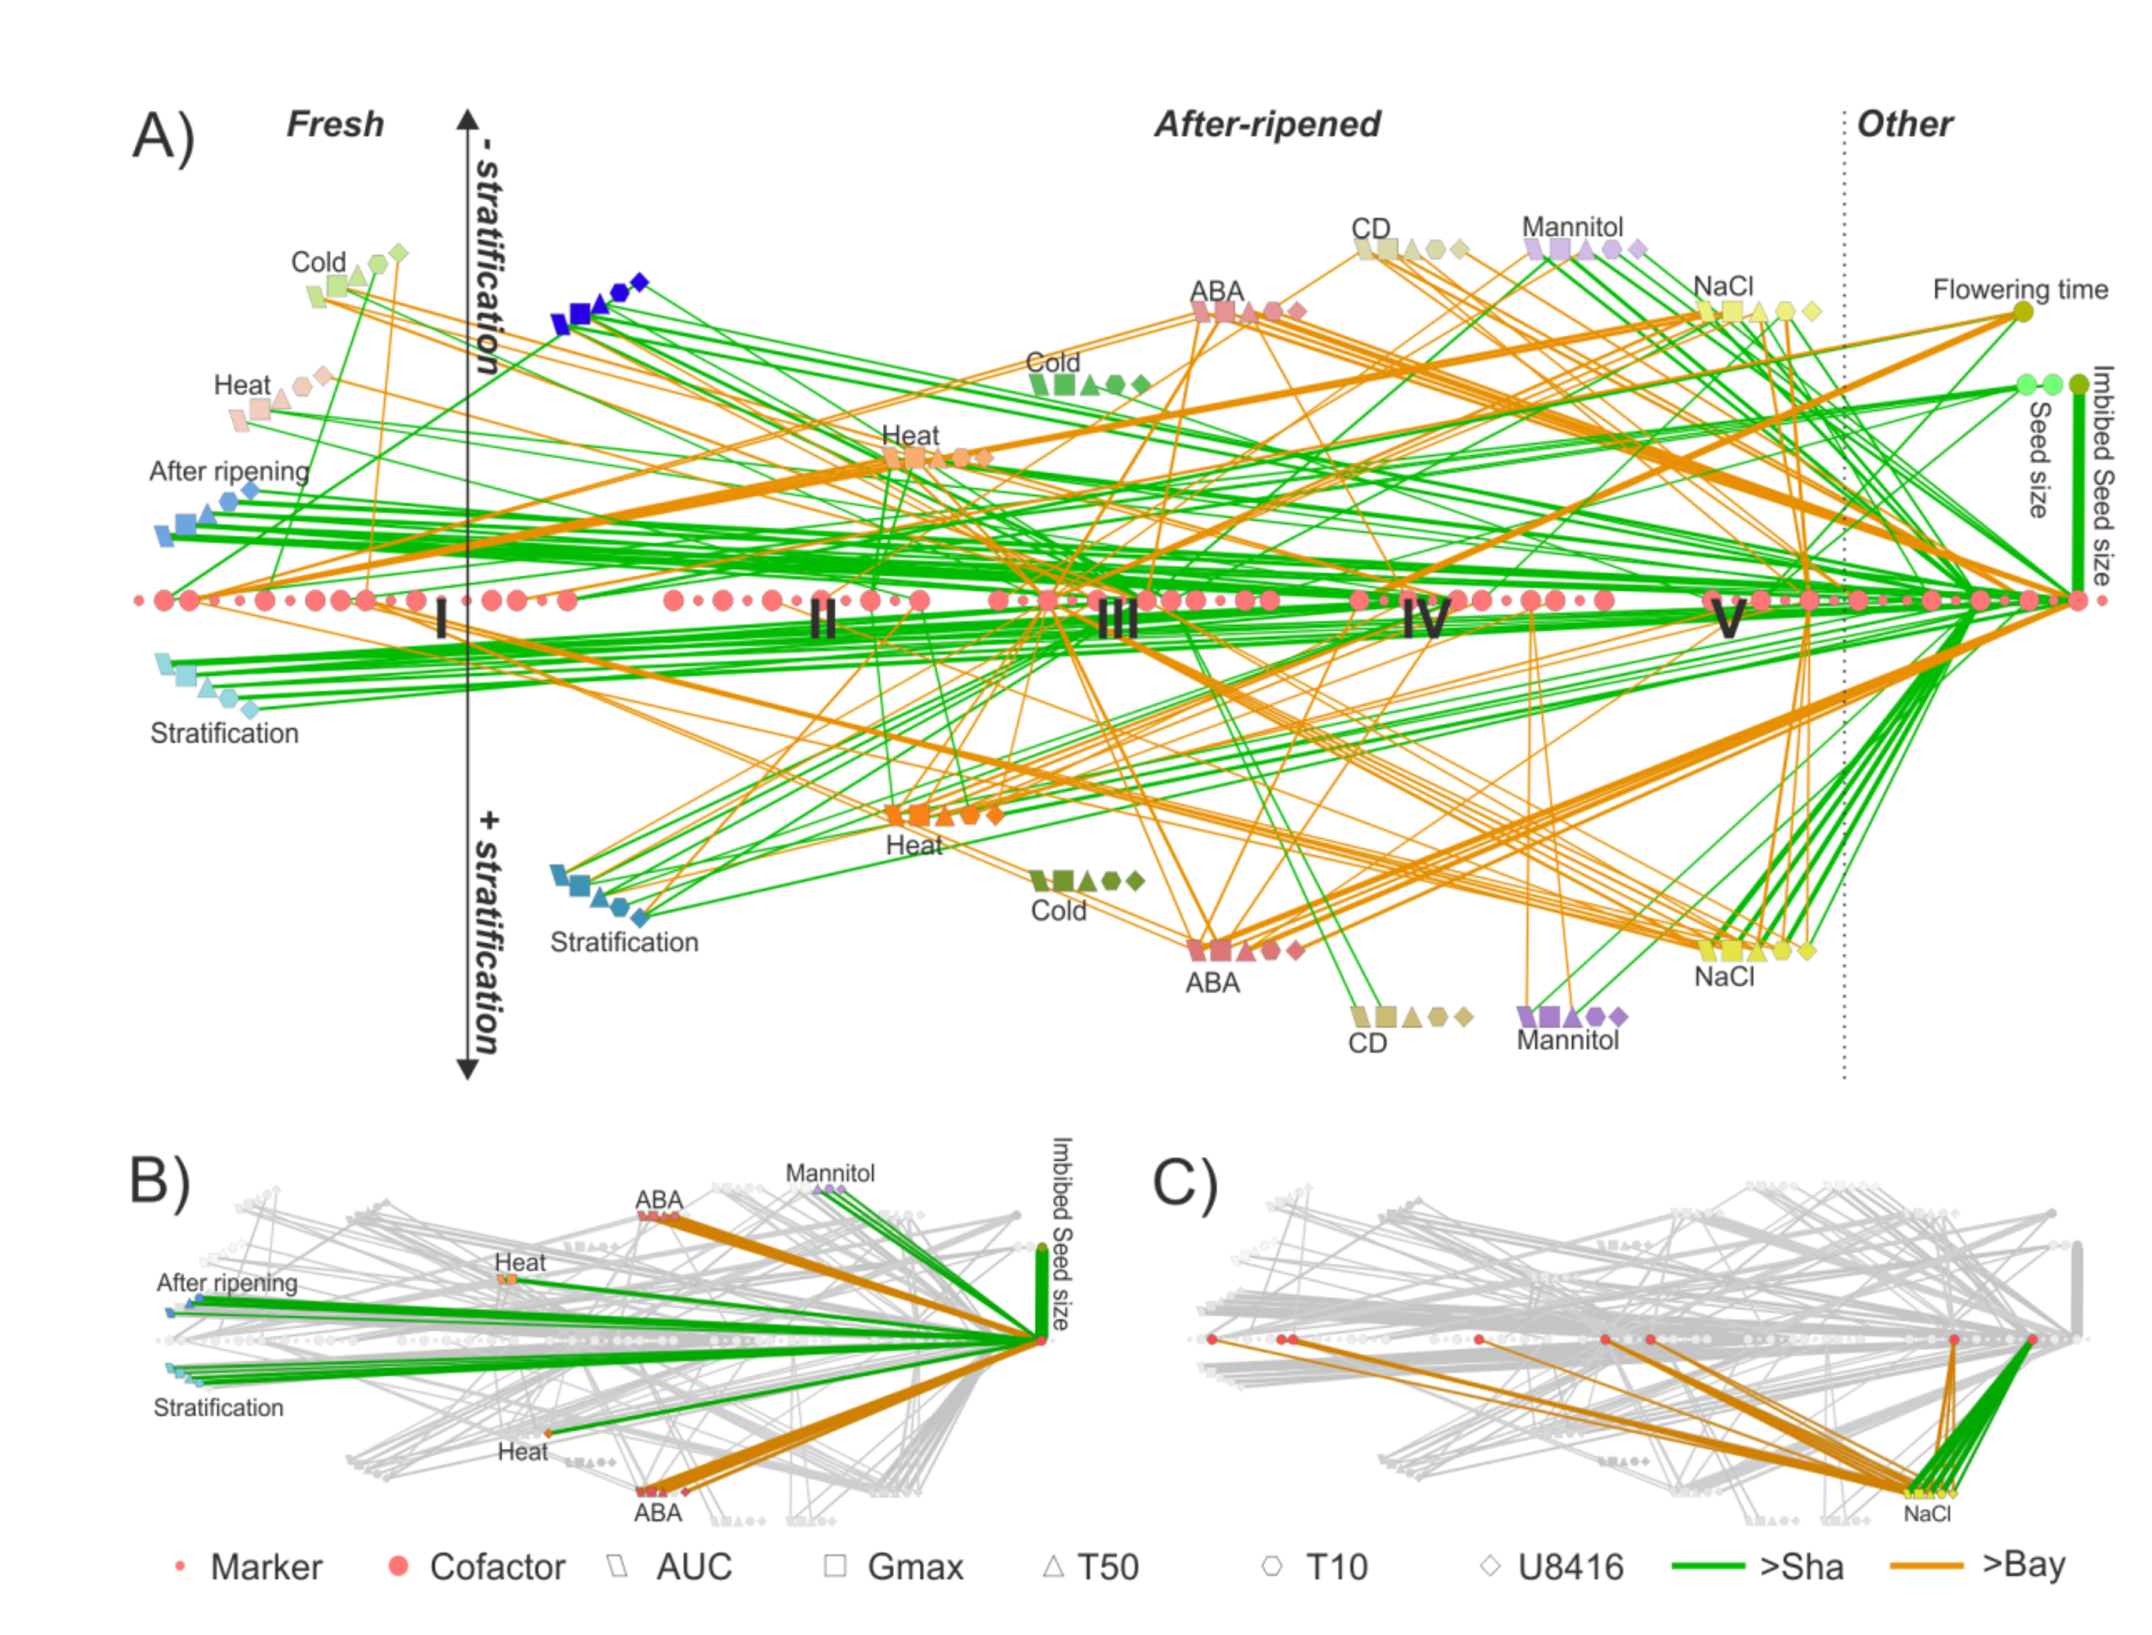
\includegraphics[keepaspectratio,scale=0.30]{eps/image_3_1_5.eps}
  \caption[Cytoscape marker trait network.]{Cytoscape Marker-Trait network. A) Significant QTL positions are 
          indicated by a connection between traits and markers, edge colors indicate the direction of the QTL 
          effect, line width indicates the LOD score; B) Sub- network showing all traits with a significant 
          QTL at marker MSAT519; C) Sub- network showing all markers with significant QTL for germination on 
          NaCl with stratification.}
\end{figure}

\begin{figure}[h!]
  \centering
  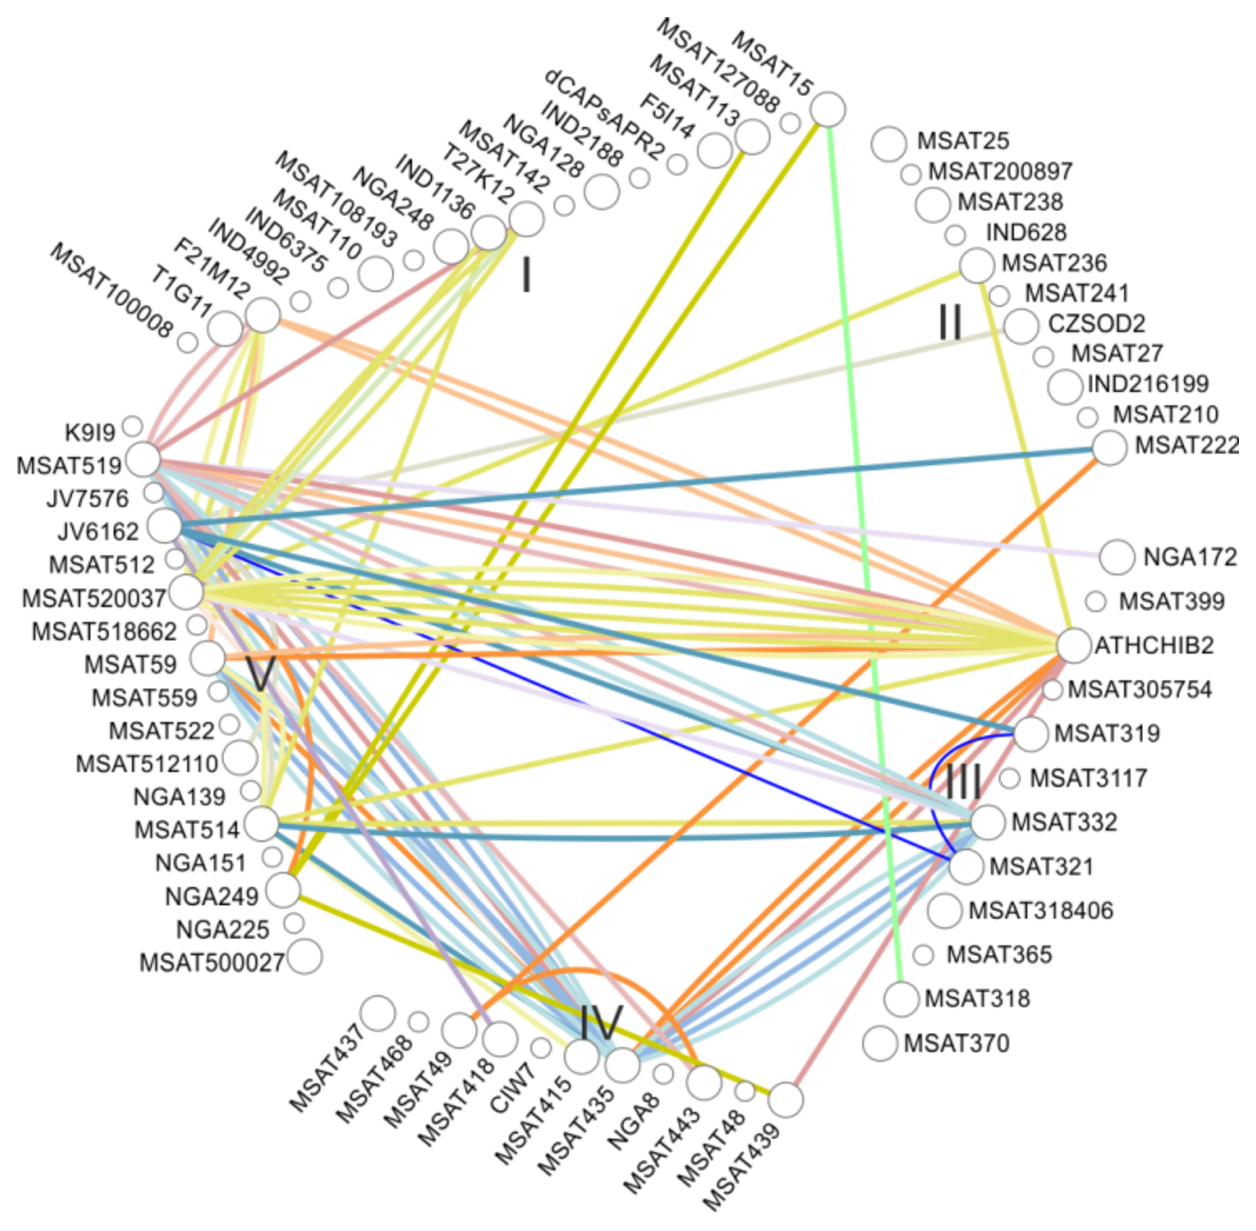
\includegraphics[keepaspectratio,scale=0.30]{eps/image_3_1_6.eps}
  \caption[Epistatic interaction network.]{Epistatic interaction network created with Cytoscape from the 
          interaction.sif output file. Nodes indicate markers (small circles) and selected cofactors (large 
          circles). Edges represent the detected significant epistatic interactions (edge colors represent 
          traits, see table \ref{table:codes} for colors).}
          \label{fig:epistaticinteractions}
\end{figure}

\subsubsection{QTLxEnvironment interaction}
To obtain a parameter for the response, we had to correct all values with their proper control condition 
values. This sometimes led to complex interpretation, which can be circumvented by using the non-corrected 
germination parameters and model them over the various environmental conditions that were tested. Because 
several environments are taken into account simultaneously the statistical power to detect loci that are 
affected by several environments increases and interpretation becomes more intuitive as the need for 
correcting the stress response by the control response is eliminated. By using this approach the 
sensitivity of a specific QTL for environmental conditions can be determined for each separate germination 
parameter. Details about the procedure are described in Material and Methods. Results are summarized in 
figure \ref{fig:gegenomewide}. The final model P-value profiles (top panel, Fig. \ref{fig:gegenomewide}) clearly show the great consistency 
between the 5 germination parameters that we measured. However, a closer look also reveals loci that 
are affecting different germination curve parameters. For example, the QTL on top chromosome 5 is not 
detected by measuring maximum germination but is well defined when using $t_{50}$ or $t_{10}$ as parameter. As 
expected, the parameter AUC (Area Under the Curve) is outperforming the others as it represents a 
combined value for maximum germination percentage, rate and uniformity. For comparison of the 
environment-specific QTL effects for the 5 different germination parameters (5 lower panels, Fig. \ref{fig:gegenomewide}) 
the effects could be compared with germination under control conditions. For example, after ripened 
seeds without stratification (AR.NS) can guide as reference for the stress treatments (AR.NS.ABA, AR.NS.CD, 
AR.NS.Cold, AR.NS.Heat, AR.NS.Mannitol, AR.NS.NaCl). The same analogy holds true for after ripened seeds
without stratification (AR.NS) and freshly harvested seeds without stratification (Fresh.NS). In this way 
stress specific QTLs on chromosome II and top chromosome III can easily be identified. Interestingly, some 
QTLs, including germination at low temperature (top chromosome I) and germination in the presence of 
exogenous ABA (bottom chromosome V) displayed opposite effects on germination when compared to the 
other treatments.

\begin{figure}[h!]
  \centering
  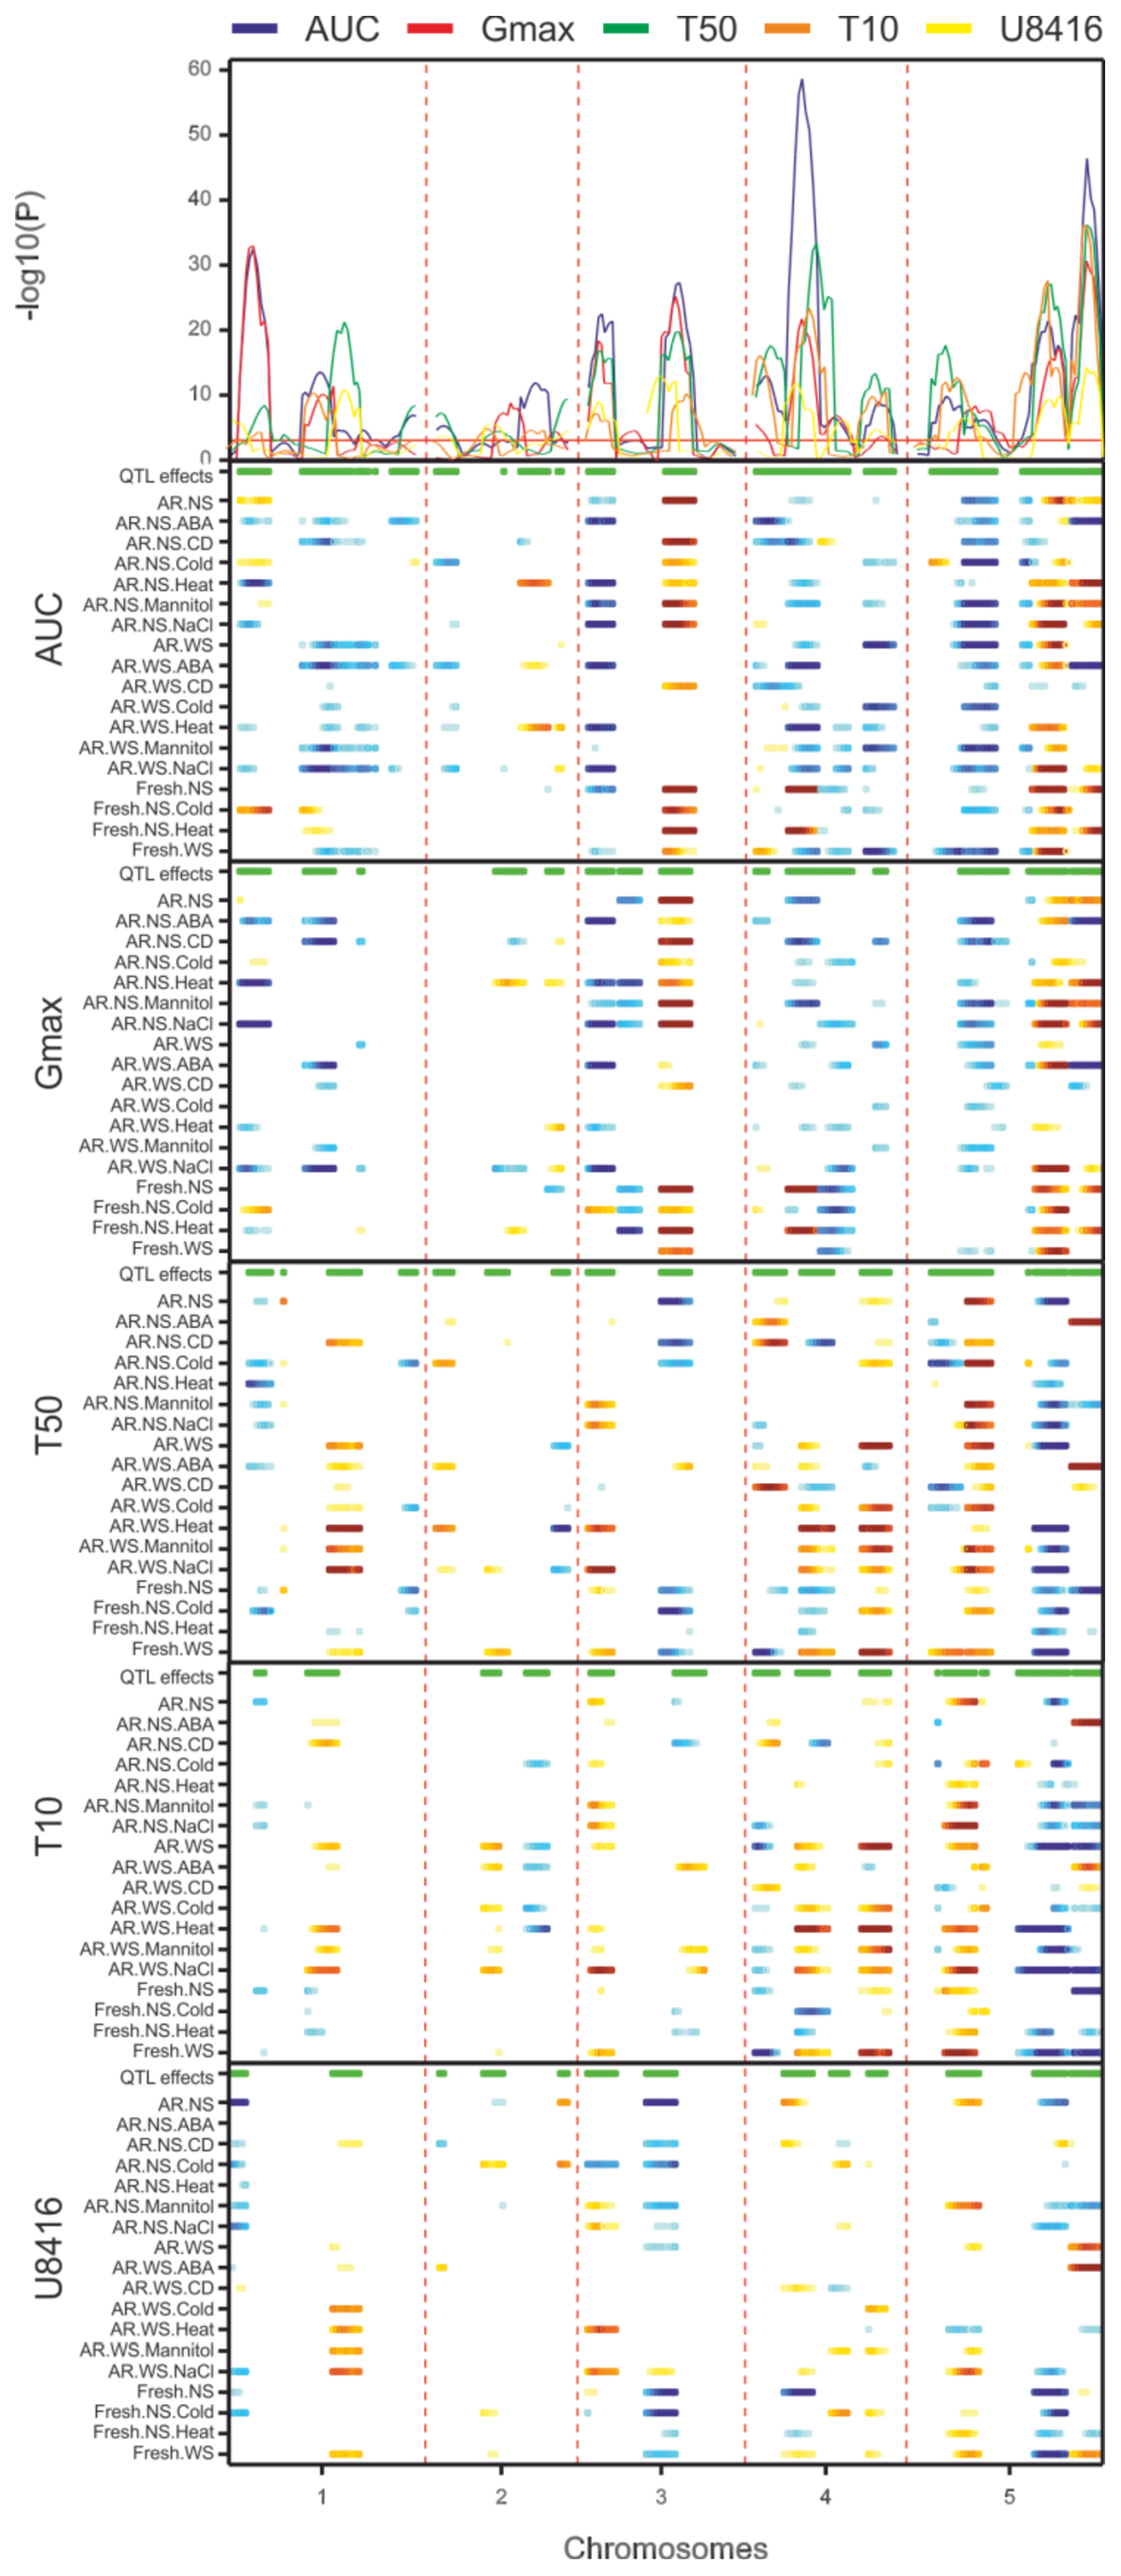
\includegraphics[keepaspectratio,scale=0.30]{eps/image_3_1_7.eps}
  \caption[G:E genome wide QTL scan.]{Genome scan for QTLxEnvironment effects for seed germination. The P-values for 
          the main effects of the different germination parameters are shown in the top panel. The red horizontal line 
          is the genome wide significance threshold. The 5 bottom panels show the environment specific QTL effects. 
          The green line indicates significant environment specific effects. For both Gmax and AUC a bigger effect of 
          the Sha allele is indicated in yellow-red (Bay-0 in cyan-blue). The color scale is opposite for the t50, 
          t10 and U8416 parameters due to the inverted nature of these parameters.}
          \label{fig:gegenomewide}
\end{figure}

\subsubsection{QTL confirmation}
Taking advantage of the residual heterozygosity present in the F6 generation of the Bay-0 x Sha population, 
combined with the large population size, we were able to confirm several QTL following the heterogeneous 
inbred family (HIF) approach. In short, RIL lines which are heterozygous at the locus of interest were 
selected in the next generation for lines homozygous for both parental alleles. These 'families' are 
near isogenic lines (NIL) which can be used to confirm the observed allelic effects (Fig. \ref{fig:confirmation}A). We 
applied this strategy for 7 of the major QTL that we detected in  this study and tested the 5 germination 
parameters for 11 different conditions. For a single parameter (Gmax) and a single HIF (line HIF103) the 
analytical procedure is summarized in figure \ref{fig:confirmation}B. We 
detected a vast QTL for imbibed seed size at the bottom of chromosome 5, which could be confirmed by the 
use of HIF103. Upon imbibition seeds swell due to rapid water uptake and possibly because of the 
expansion of the inner mucilage layer. In Sha, which is a natural mutant for the MUM2 gene 
\cite{Macquet:2007}, this swelling did not occur. Also the HIF lines at the MUM2 position showed a 
clear difference in swelling phenotype which was still significant 24 hours after imbibition (Fig. \ref{fig:swelling}).

\begin{figure}[h!]
  \centering
  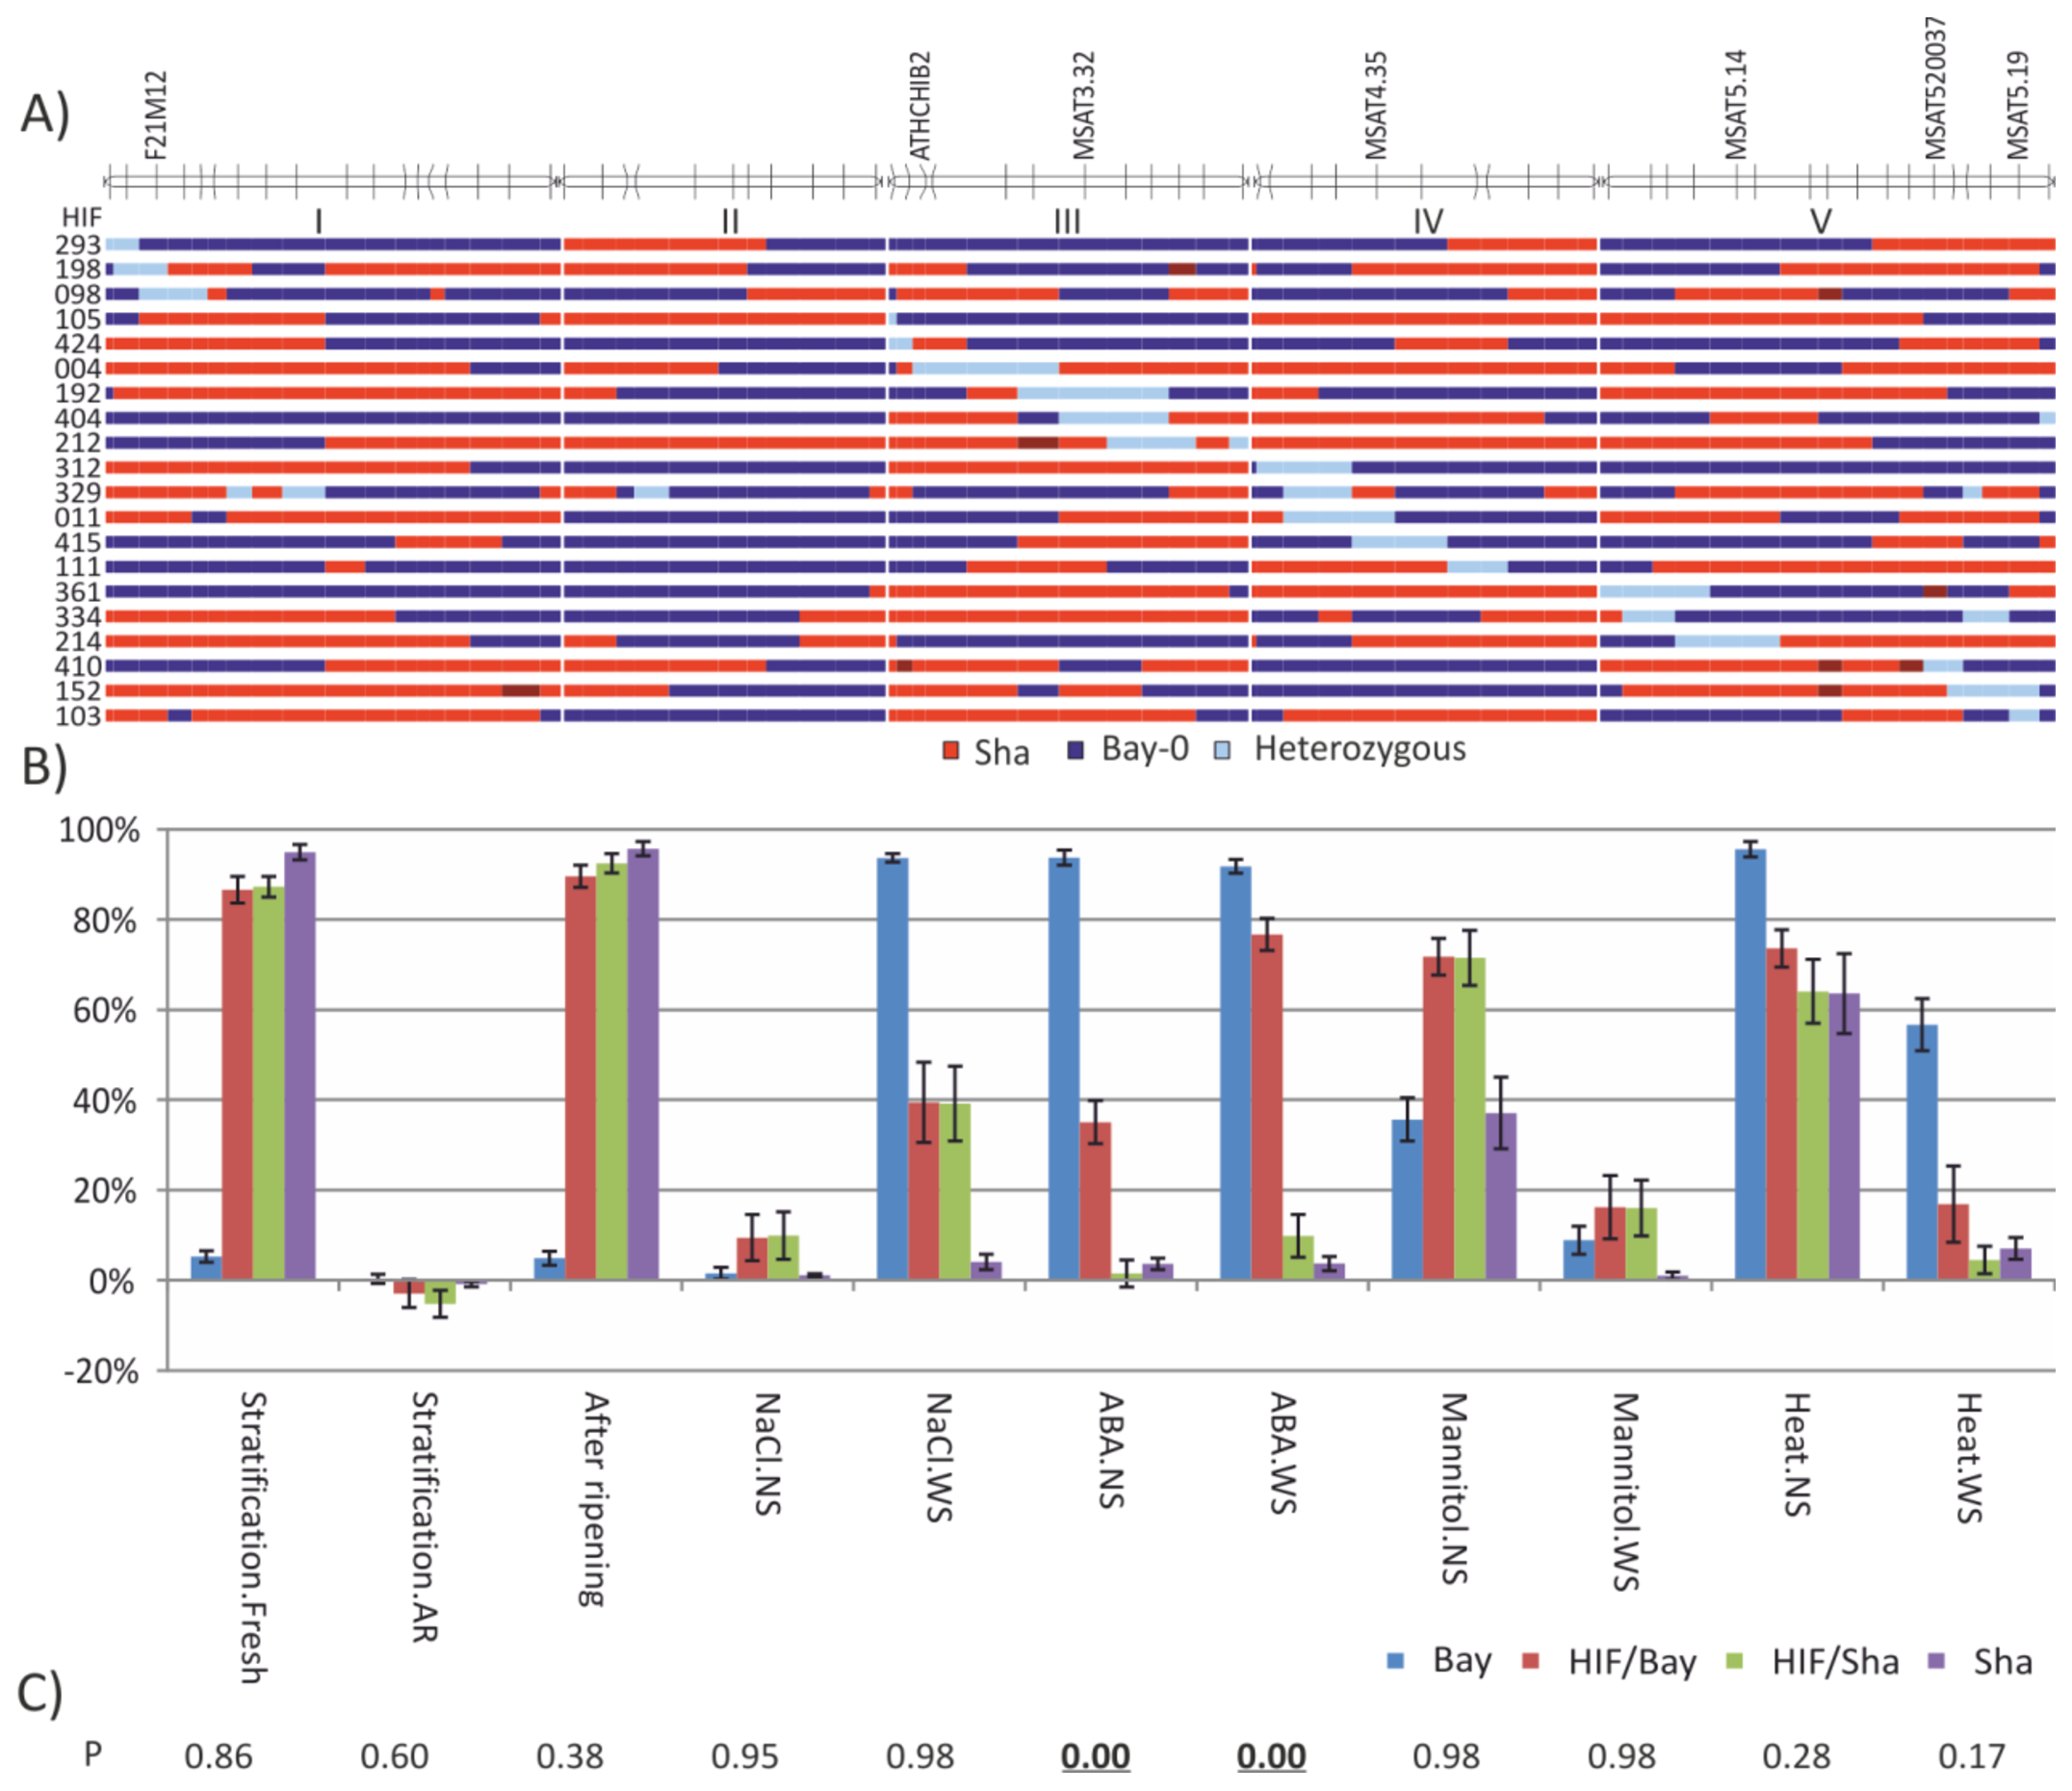
\includegraphics[keepaspectratio,scale=0.30]{eps/image_3_1_8.eps}
  \caption[QTL confirmation.]{Example of the confirmations performed with the HIF approach. A) The blue/red bars 
          indicate the allelic confirmation of the HIF lines used (blue=Bay-0, red=Sha, light blue=segregating). 
          The 5 chromosomes are indicated at the top with the nearest genetic marker for the 7 major loci. B) example 
          analysis for HIF103 (segregating at MSAT5.19, bottom chromosome V). Indicated is the maximum germination 
          (Gmax) for 11 conditions. Error bars represent standard error of at least 6 replicates. Responses are 
          calculated by subtracting the test sample from the control sample as indicated in table \ref{table:codes}. C) T-test 
          significance values for the response values (significant (P<0.05) values are bold).}
          \label{fig:confirmation}
\end{figure}

\begin{figure}[h!]
  \centering
  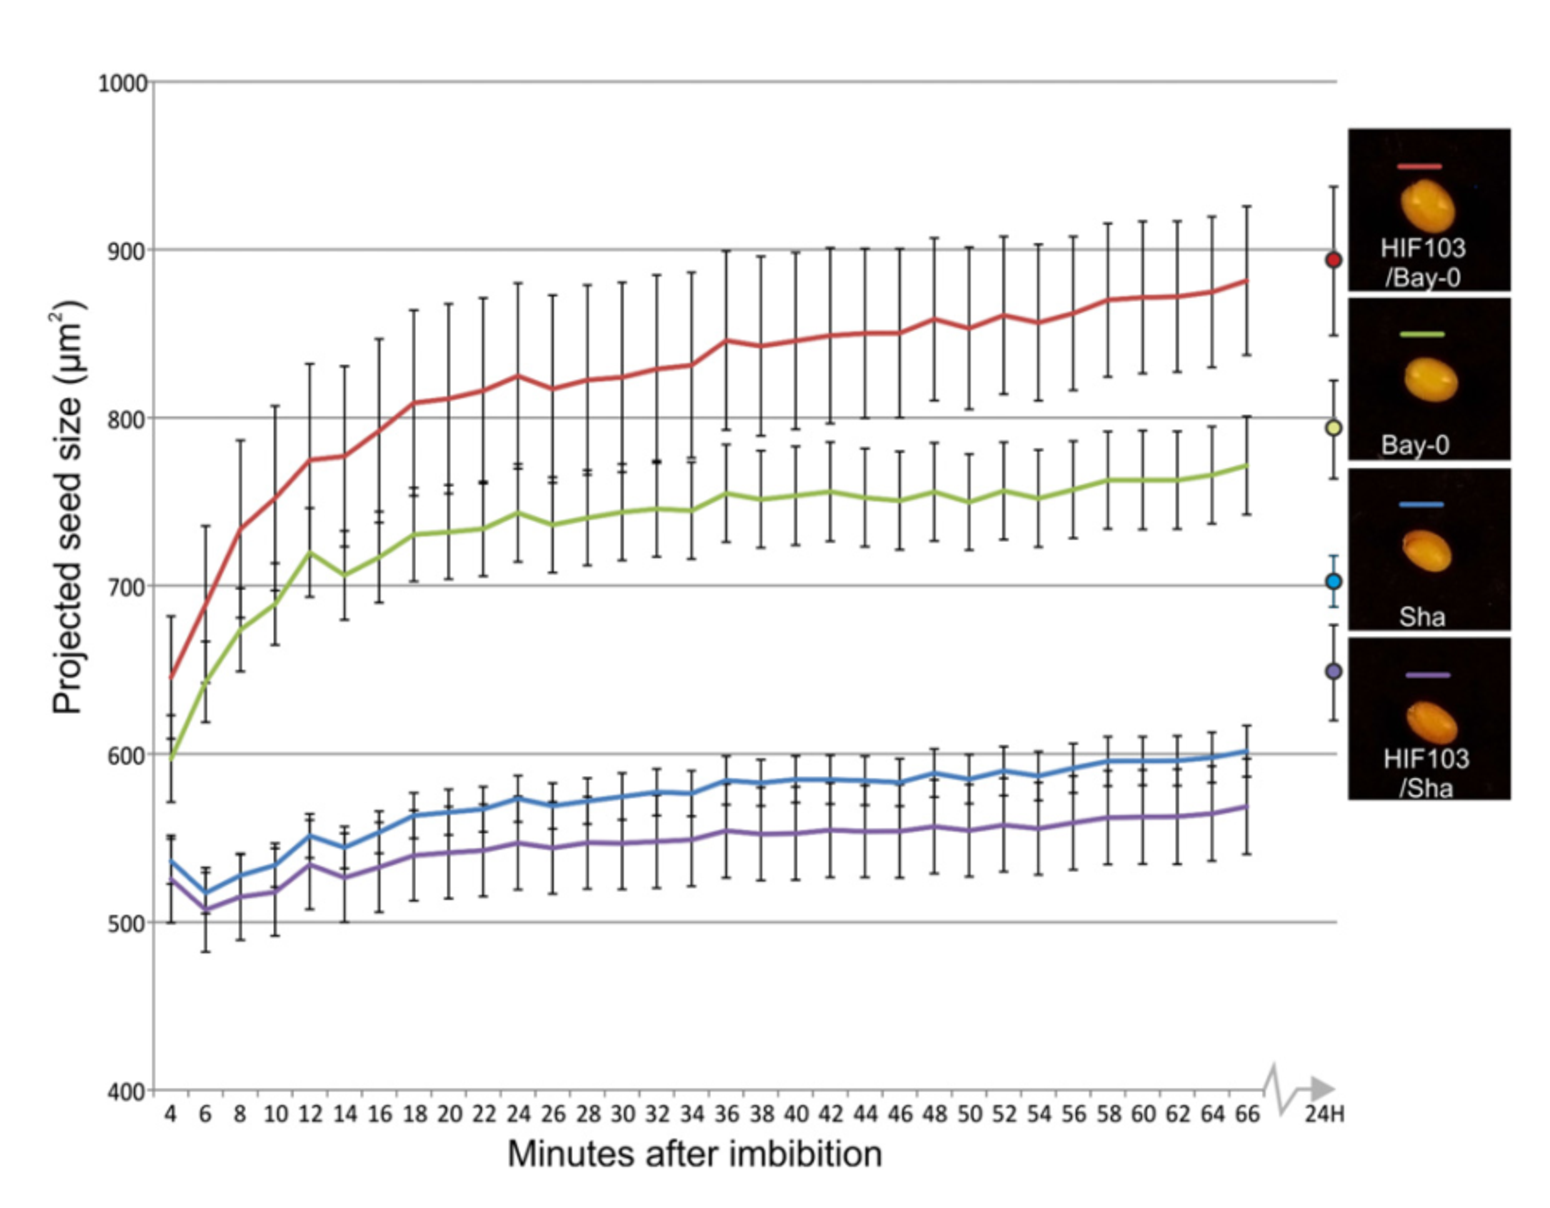
\includegraphics[keepaspectratio,scale=0.30]{eps/image_3_1_9.eps}
  \caption[Seed Swelling.]{Different increases in seed size during the start of imbibition for Bay-0 (green), Sha (blue), 
          HIF103/Bay-0 (red), and HIF103/Sha (purple) seeds. Shown is the average projected seed size area of 10 seeds. 
          Error bars represent SE values. Photographs show 24-h imbibed seeds.}
          \label{fig:swelling}
\end{figure}

\subsection{Conclusions and Discussion}
When analyzing large (RIL) populations, it is hardly feasible to manually count all germination 
experiments several times a day to obtain germination curves. Therefore, previous studies mostly 
restricted to counting end-point germination \cite{Quesada:2002, Alonso-Blanco:2003, Clerkx:2004, 
Laserna:2008, Meng:2008, Bentsink:2010, Galpaz:2010, Vallejo:2010}. A germination curve allows QTL 
mapping under conditions where rate and uniformity are delayed, but maximum germination is not 
affected. Therefore, we used the Germinator package \cite{Joosen:2010} that enabled measurement 
of cumulative germination data and extracting 5 germination parameters that describe the resulting 
germination curve. In the present study we describe several germination QTLs that were not detected 
before in the Bay-0 x Sha population. We observed interesting co-localizations for several germination 
traits and identified the loci that show large effect epistatic interactions. Among these were new 
loci and loci similar to the ones already found in other RIL populations (see \cite{Joosen:2011} - Table 4 for 
the major identified QTL loci).

\subsubsection{Dormancy}
Primary dormancy has been studied extensively in various RIL populations \cite{Bentsink:2010}. These 
authors quantified primary dormancy with the DSDS50 parameter (days of dry storage to reach 50\% 
germination), which is a good measure for after-ripening related dormancy breaking. Although we only 
compared the germination characteristics of freshly harvested seeds with those of after ripened 
seeds and fresh seeds with and without stratification, we detected large genetic variation. Both 
dormancy breaking treatments showed strong QTL at positions 3-2, 4-1 and 5-2, co-locating with DOG6, 
DOG18 and DOG1, respectively (See \cite{Joosen:2011} - Table 4). DOG18 was not detected in a Ler x Sha population and showed a 
stronger dormancy in Ler as compared with An-1, Fei-0 and Kas-2 \cite{Bentsink:2010}. We detected stronger 
dormancy in Sha as compared to Bay-0 at the DOG18 locus. This suggests that both Ler and Sha contain 
an allele of similar strength which is stronger when compared to An-1, Fei-0,  Kas-2 and Bay-0. Remarkably, 
for both the DOG6 and DOG18 location the sensitivity to ABA was higher in Bay-0, whereas dormancy was 
deeper in Sha, which resulted in a directional change of the QTL effect. The more dormant Sha parent 
contains higher initial ABA levels and apparently, after-ripening and 
stratification reduce the ABA sensitivity to a greater extent as compared to the Bay-0 parent. This 
effect was not observed for the DOG1 locus. Further, we identified a strong effect of the dormancy-
breaking treatments on the initiation (t10) and rate (t50) of germination at the bottom of chromosome 5 
(marker MSAT519, 85 cM). The same was observed for germination on mannitol and germination at higher 
temperature. A QTL with opposite effect at this position was found for germination on ABA. Interestingly, 
these co-located with a QTL found for imbibed seed size. 

\subsubsection{Water uptake}
Initiation and rate of germination are highly influenced by the overall water potential of the seed. The 
mucilage layer surrounding the seed appears to play an important role in the process of water uptake 
\cite{Penfield:2001}. Sha is a natural mucilage mutant due to a mutation in the MUM2 gene, which changes 
the hydrophilic potential of rhamnogalacturonan I \cite{Macquet:2007}. Although mucilage has been reported 
to be dispensable for germination and development under lab conditions \cite{Arsovski:2010}, a link with 
germination under reduced water potential conditions was shown by \cite{Penfield:2001}. They showed 
reduced maximum germination of a mucilage-impaired mutant only on osmotic PEG solutions. In our study, 
other traits that co-located on the MUM2 locus were delayed initiation and rate of germination on osmotic
mannitol solution but also on water, which clearly shows the advantage of determining a detailed 
germination curve. We also observed a very strong QTL for swelling of the seed in the first hours of 
imbibition (imbibed seed size) at the MUM2 location. Interestingly, exogenous ABA can be used to 
stimulate mucilage production and ABA-1 mutants are affected in mucilage production \cite{Karssen:1989}. 
This indicates a regulatory role of ABA in mucilage production and fits with our observation of the 
co-localization of a QTL for initiation and rate of germination with a QTL with opposite effect for ABA 
sensitivity. Therefore, we hypothesize that Sha has a slower initiation and rate of germination,
combined with reduced ABA sensitivity due to its mutation in the MUM2 gene. This observation may open 
new research strategies to define the regulatory role of ABA in mucilage production and its multiple 
effects on germination parameters.

\subsubsection{Salt, Heat and ABA}
At the top of chromosome I, underlying marker F12M12, we detected a strong QTL for maximum germination in 
the presence of 100 mM NaCl or 0.5μm ABA. A similar locus has been identified and fine-mapped in a 
Ler x Sha population \cite{Ren:2010}. They identified a premature stop codon in the Response to ABA and 
Salt 1 gene (RAS1; At1g09950) in Sha that led to a truncated protein and showed its role as a negative 
regulator of salt tolerance during seed germination and early seedling growth by enhancing ABA 
sensitivity. Here we show that a similar locus is also inferring tolerance to germination at 30\degree C. 
This suggests an additional role for the RAS1 gene. Increased heat tolerance due to modulation of 
ABA sensitivity has been shown before for other loci, \cite{Argyris:2008,Lee:2010}. 
Interestingly, our present study showed a strong effect of stratification which resulted in a strong 
reduction of significant linkage for NaCl, heat and ABA sensitivity at the F12M12 locus. A specific 
QTL for germination on NaCl preceded by a cold stratification period was found at the middle of 
chromosome I (marker T27K12). Also at this locus we found colocation with sensitivity for germination 
on ABA after stratification. Further fine-mapping at this locus might help to elucidate the effect 
of stratification on ABA mediated abiotic stress tolerance, as well as the apparent overlap of 
dormancy and stress responses. Especially interesting is QTL 5-1 (See \cite{Joosen:2011} - Table 4, and Fig. \ref{fig:gegenomewide}) which mainly 
influences rate and initiation of germination. We detected this QTL for t50 in after ripened seeds 
with stratification treatment, but also for t10 and t50 for germination on salt, regardless of a 
preceding cold stratification and for maximum germination after an accelerated aging treatment. 
One of the genes underlying this QTL interval is a nicotinamidase gene (NIC2, At5g23230), the mutant 
of which has retarded germination and impaired germination potential \cite{Hunt:2007}. These 
authors suggested that NIC2 is normally metabolizing nicotinamide during moist chilling or 
after-ripening, which relieves inhibition of poly(ADP-ribose) polymerase (PARP enzyme) activity and 
allows DNA repair to occur prior to germination. Both accelerated aging and germination under salt 
stress conditions might require optimal functioning of this DNA repair mechanism. Further research 
is needed to determine whether NIC2 is causal for this QTL.

Detection of epistatic interactions in genetic studies can enhance the understanding of underlying 
molecular mechanisms. Recently, \cite{Galpaz:2010} showed strong epistasis in the genetic network 
controlling germination under salt stress in Arabidopsis. Due to careful dissection of the epistatic 
relationships they were able to show that three detected QTL rely on the presence of a Columbia 
allele at a QTL on top of chromosome 1. This observation led to the hypothesis that RAS1 
\cite{Ren:2010} functions as a switch of the genetic network by regulating the expression of the 
other QTL. In another study it was found that epistasis significantly influences both fitness and 
germination in Arabidopsis \cite{Huang:2010} and novel allele combinations were identified that 
resulted in higher fitness. In our study we detected clear hotspots of epistatic interactions 
between QTL loci on chromosome 3, 4 and 5 (ATHCHIB2, MSAT332, MSAT435, MSAT520037 + MSAT519, 
respectively). This observation strengthens the hypothesis that some of the traits with strong 
QTL co-localizations indeed rely on the same underlying genetic networks.

\subsubsection{Concluding remarks}
We analyzed natural variation for many seed germination characteristics and showed their correlation, 
(shared) QTL positions and epistatic interactions, using a high-throughput phenotyping approach and 
subsequent high-throughput QTL mapping. Using the HIF approach, confirmation of some major QTL 
hotspots was demonstrated, which allows a fast but solid confirmation of a QTL position. Together 
with results from several other studies focusing on genetic variation in seed traits, this study 
has generated an extensive QTL database for Arabidopis and proposed a method of analysis to 
visualize the genetic landscape of seed performance. This database is a solid resource for further 
study. For most of the found loci in this and other studies further characterization, and in most 
cases fine mapping, must be undertaken to elucidate the causal molecular mechanisms. Further, we 
have designed a free available analysis protocol to perform detailed high-throughput QTL analysis 
based on the R/qtl MQM routine. In this era of large-scale phenotyping we regard a detailed analysis 
of QTL, QTLxQTL and QTLxEnvironment interaction as indispensable steps to allow visualization 
and interpretation of multiple traits.



\section{Metabolites in a DesignGG experiment}
A complex phenotype such as seed germination is the resultant of several genetic and environmental 
cues and requires the concerted action of many genes. The use of well-structured recombinant inbred 
lines in combination with omics analysis can help to disentangle the genetic basis of such 
quantitative traits. This so called genetical genomics approach can effectively capture both 
genetic (G) and epistatic interactions (G:G). However, to understand how the environment interacts 
with genomic encoded information (G:E) a better understanding of the perception and processing of 
environmental signals is needed. In a classical genetical genomics setup this requires replication 
of the whole experiment in different environmental conditions. A novel generalized setup overcomes 
this limitation and includes environmental perturbation within a single experimental design. 

We developed a dedicated QTL mapping procedure to implement this approach and used existing 
phenotypical data to demonstrate its power. Additionally, we studied the genetic regulation of 
primary metabolism in dry and imbibed Arabidopsis seeds. Many changes were observed in the 
metabolome which are both under environmental and genetic control and their interactions. 
This concept offers unique reduction of experimental load with minimal compromise of statistical 
power and is of great potential in the field of systems genetics which requires a broad 
understanding of both plasticity and dynamic regulation.

\subsection{Introduction}
The use of natural variation to disentangle the genetic (G) mechanisms underlying phenotypic differences 
has been very successful both in crop plants and in the model plant Arabidopsis (Arabidopsis thaliana; 
\cite{Alonso-Blanco:2009}. Most of the variation within wild or domesticated plant species is of 
quantitative nature determined by G polymorphisms at multiple loci. Such quantitative trait loci (QTL) 
can beanalyzed efficiently using experimental mapping populations such as recombinant inbred lines (RILs)
derived from directed crosses. Nowadays, many wellstructured RIL populations are available, often 
accompanied with detailed studies of phenotypic variation (Mitchell-Olds and Schmitt, 2006). The complexity 
ofquantitative traits is further determined by the interactions between genomic loci (i.e. epistasis) and 
between the genotype and the environment (genetic X environmental [G:E]). While epistasis can be effectively
identified in QTL analyses, albeit with lower power than main effects, the detection of G:E interactions 
requires experimentation in multiple conditions of interest. Because of the large population sizes often 
needed to obtain sufficient statistical power for QTL detection, G:E interactions are usually ignored in 
experimental setups. However, a better understanding of the perception and processing of environmental (E)
signals is greatly needed, because interactions provide important insights in adaptation mechanisms and
evolutionary constraints such as balancing and disruptive selection. To obtain a more detailed view of the
molecular mechanisms underlying phenotypic variation, genetical genomics studies, in which molecular traits
are genetically analyzed, have been successfully applied to enhance a directed strategy to identify causal
relationships (Kliebens tein et al., 2006; Keurentjes et al., 2007a; van Leeuwen et al., 2007; 
Wentzell et al., 2007; West et al., 2007; Rowe et al., 2008). The observed phenotype is often the resultant 
of a functional cascade of gene transcription followed by protein translation and modification, which 
finally leads to a highly dynamic metabolome underlying emergent properties (Kooke and Keurentjes, 2011). 
With the technological advances made in genomic analytical platforms, such as transcriptomics, proteomics, 
and metabolomics, the large-scale, high-throughput analyses needed for quantitative G approaches have 
become feasible (Jansen and Nap, 2001; Keurentjes et al., 2008). 

Incorporating developmental and E  perturbation in the often expensive and laborious omic analyses, an 
alternative experimental setup, coined generalized genetical genomics (GGG), using balanced fractions 
of a RIL population has been proposed (Li et al., 2008). It provides a cost-effective experimental setup 
for hypothesis-generating research in multiple environments. Such an approach aims for the creation of 
subpopulations of RILs, one for each environment to be tested, with an optimal distribution of parental 
alleles over all available markers (Li et al., 2009). When these subpopulations are subjected to E 
perturbation, the emerging phenotypes can be explained by several sources of variation: G variation, 
E variation, and G:E variation. Whenever the resulting phenotype is not or only mildly affected by E 
interactions (G:E), the analysis of the different subpopulations can be combined, gaining the full power 
of a complete population. However, when a trait shows strong G:E interaction (e.g. those that only express G variation in specific 
environments), the power to detect QTL is dependent on those subpopulations expressing the G variation. 
Although G:E interactions have been detected previously in genetical genomics studies for expression 
(Li et al., 2006; Smith and Kruglyak, 2008; Gerrits et al., 2009; Yeung et al., 2011) and metabolite 
content (Zhu et al., 2012) by analyzing all lines in a population under different environments, the 
GGG concept offers an effective way of studying a combination of G and E perturbations and is of great 
potential in the field of systems genetics, in which a broad understanding of both plasticity and
dynamics is required (Li et al., 2008). The fundamental basis of the experimental design and data 
analysis using a full model ($Y = E + G + G:E + e$), where $Y$ is the observed phenotype and $e$
is residual error, is generally valid and frequently used (Churchill, 2002; Li et al., 2006; Gerrits
et al., 2009). As a proof of principle, we present experimental data on the G regulation of primary 
metabolism in dry and imbibed Arabidopsis seeds using a GGG design and discuss the application and 
implications of such a strategy.

Plants are extremely rich in biochemical compounds, and major roles in plant development, adaptation, 
and defense have been identified for biosynthesis pathways and their products (Binder, 2010). The 
biosynthetic pathways of primary metabolites are well studied and often well conserved between 
different taxa (Peregrín-Alvarez et al., 2009). Nonetheless, quantitative variation for many of 
these compounds can be observed between natural variants, which might be reflected in their different 
growth characteristics. The



\chapter{High throughput QTL mapping using correlated traits}
\thispagestyle{empty}
\label{chap:ctlmapping}

\emph{In this chapter we develop a new methodology to be used in quantitative genetics 
called Correlated Traits Locus (CTL) mapping, a method complementary to QTL mapping. 
Where QTL associates differences in mean, CTL, associate differences in correlation to 
genetic variation, i.e. CTL identify regions in the genome for which one genotype leads 
to correlated expression between a pair of traits, while the other genotype shows none 
(or significantly different) correlation.}

\null
\vfill

\begin{myexampleblock}{In press:}
  \authors{Danny Arends, Pjotr Prins, Yang Li, Lude Franke and Ritsert C. Jansen}\\
  \emph{CTL mapping}\\
  \bold{Unknown} (XXXX)\\
  \authors{Harm-Jan Westra*, Danny Arends*, ... ,  Ritsert C. Jansen and Lude Franke}\\
  \emph{Identification of neutrophil mediated eQTLs from whole blood, without the need to sort cells}\\
  \bold{Nature Methods} (2013)
\end{myexampleblock}

\newpage

\section{Introduction}
  QTL mapping of a gene expression identifies regions in the genome at which different genotypes lead to differences in gene
  expression levels. In a similar fashion, abundance of thousands of proteins and metabolites can be measured to map protein 
  QTL (pQTL) and metabolite QTL (mQTL). 
  Deep sequencing, chromatin, and methylated DNA immunoprecipitation are just a few of the latest technologies that add to 
  the arsenal of tools available for the study of the genetic variation underlying quantitative phenotypes. Together, eQTL, 
  mQTL, and pQTL are referred to as xQTL \cite{Arends:2012}. Different xQTL can localize to confirm each other, for example, 
  with the \emph{A. thaliana} glucosinolate pathway \cite{Jansen:2009}. Such inference can lead to dissecting pathways and gene networks, 
  currently an active field of research \cite{Prins:2012}.

  Advances in QTL mapping focus on increasing QTL detection power and precision by using more and more advanced models to explain 
  observed variance. A higher amount of explained variance will result in a more reliable causal inference \cite{Li:2010}. Methods 
  developed to improve this explained variance are: Bayesian interval mapping, a framework to add prior knowledge \cite{Yandell:2007, 
  Hageman:2011}, Multiple QTL model (MQM) mapping tries to improves power by fitting a genetic model using backward elimination of 
  pre-selected genetic loci\cite{Jansen:1993, Arends:2010} and machine learning approaches, such as randomForest \cite{Bureau:2003}, 
  support vector machines (SVM), neural networks, and more recently vQTL mapping \cite{Valdar:2011} fall into this class of methods
  developed to improving power and attribute more variance to genetic factors.

  Another class of methods used in QTL mapping are the multivariate mapping approaches. These approaches combine variance information 
  from multiple traits to increase the number and significance of detected QTL. Methods like principal component analysis (PCA) and 
  differential expression (DE) analysis fall under the multivariate mapping methods. A review of many of these methods can be found 
  in Gilbert and le Roy \cite{Gilbert:2003}.

  Recently the field of creating differential networks has gained more and more attention. In these approaches the differences 
  between genetic networks are studied \cite{Fuente:2010,Horvath:2008}. Several approaches have been used to identify differential 
  correlations between experimental conditions for large-scale omics datasets using topological overlap \cite{Tesson:2010}. However 
  current approaches for detecting differential correlations only focus on the detection of differences in correlations between 
  two (or more) experimental conditions \cite{Fukushima:2013, Tesson:2010,Horvath:2008}. 

  We however believe that a major source of complementary information is available. Here, we present Correlated Traits Locus (CTL) 
  mapping, a method complementary to QTL mapping. Where QTL associates differences in mean, CTL, associate differences in correlation to 
  genetic variation, i.e. CTL identify regions in the genome for which one genotype leads to correlated expression between a pair of 
  traits, while the other genotype shows none (or significantly different) correlation. CTL information complements QTL information, 
  and provides insights into the genetic regulation of correlated traits, hidden in a traditional QTL mapping approach.
  
  %CTL mapping closes the gap between classical QTL mapping and differential network analysis by using the genotype as experimental 
  %conditions. At each genetic locus we divide our population in two genotype conditions, allowing us to map differential networks 
  %when only a single experimental condition is available. Added advantage of this approach is that CTL mapping allows us to detect 
  %which genetic locus is responsible for the difference in observed correlation.

  CTL mapping using the R/ctl package is performed in the same way as QTL mapping using the R/qtl \cite{Broman:2003, Arends:2010} 
  package. This means data and results from R/qtl are directly usable in the R/ctl package. The results section shows a small code 
  example, to show similarities between CTL mapping and QTL mapping using R/qtl.

\section{Calculating a CTL}
  A CTL is calculated at marker M by analyzing all possible phenotype-phenotype combinations. The input for the calculation is 
  the genotype of marker M and the phenotypes measured on the individuals. Rather than taking the mean phenotype value for each 
  of the genotypes, as is done with QTL mapping, correlation is calculated between p1 and p2 only for individuals with the 
  A allele, we do the same for the individuals with the B allele. In pseudo code:
\begin{verbatim}
    foreach p1 in Phenotypes
      foreach p2 in Phenotypes
        corA = cor(p1|A, p2|A)
        corB = cor(p1|B, p2|B)
\end{verbatim}
  In words: At marker M, split the individuals in two groups conditional on their genotypes. Now, for each pair of phenotypes 
  (p1 and p2) calculate the correlation between p1 and p2 using individuals with an A allele (corA) or with a B allele (corB). 
  When corA or corB is high it implies that p1 and p2 are regulated together conditional on the genotype.

  This calculation of differences in correlation using pairwise phenotypes conditional to genotype is repeated for all markers.

  For the sake of simplicity the example given here deals with a cross with only 2 alleles (A and B) CTL mapping however is not 
  limited to only two alleles (see the Discussion section).

  \subsection{Locating genetic markers acting on trait pairs}
  In itself, the difference in phenotype-phenotype correlations observed at specific markers is interesting. The correlation 
  suggests that the pair p1 and p2 are connected phenotypes. For molecular data p1 and p2 could be acting in tandem, they could 
  be in the same pathway, they could have the same regulator or they could be connected in some other way.
  Naturally, there is the possibility the correlation is there by chance, or by sequence polymorphisms \cite{Alberts:2007}.
  When the phenotypes p1 and p2 are highly correlated for both A and B, however, the genomic location at marker M may not be so
  meaningful in the context of genetics  But when correlate between expression levels varies significantly between genotype A 
  and B (e.g. $corA >> corB$), some form of regulation at marker M in genotype A in the genotype is implied.

  \subsection{Take the differential}
  Therefore, to calculate the CTL effect size, we add an extra step. CTL effect size is based on the difference between corAA and 
  corBB, i.e., the CTL effect is the delta of the correlations for the two genotypes AA and BB:

  $$ CTL = corAA - corBB $$

  Again, this CTL effect size is calculated for every genomic positions.  When at a certain genomic locations phenotypes T1 and T2 
  correlate highly in AA, but for BB do not (or significantly less) correlate there may be an effect of interest. This, in essence, 
  is a CTL. The CTL suggests the genomic location is operating on both traits in tandem for genotype (AA), but not in the other 
  genotype (BB). Therefore, a hidden factor X at the CTL location (M) may be involved controlling the correlation between the two 
  phenotypes.

  Finally, to correct for difference in sample size the full calculation reads for the CTL at markers M:
  
  $$  CTL = \frac{(Z(corAA) - Z(corBB))}{stderr} $$

  For calculation of Z and stderr see the section 'CTL analysis on N-genotypes' in the discussion.

  \subsection{Assigning significance}
  
  When scaling the difference between two Z-values using the standard error we obtain a T-statistic which follows a 
  normal distribution \cite{Biometry:1995} allowing us to calculate an exact p-value.

  This p-value still needs to be corrected for multiple testing by using a bonferroni correction or a multi-trait 
  permutation approach \cite{Breitling:2008a} to estimate the null distribution. When doing permutations in each round 
  the link between genotype and trait is broken, by redistributing at random genotypes to the individuals while not 
  allowing for duplicates. After 10.000+ permutations each CTL score is transformed into a p-value.

  Observing that a trait might show many other traits with a CTL at a marker we can also use an alternative approach: 
  Don't assign significance to the individual trait-trait connections, but summarize the effect across all traits, 
  then use Quantile-Based Permutation Thresholds \cite{Neto:2012}. Using this approach for CTL mapping will add power 
  to detect sets of co-localizing CTLs, but will obscure the individual trait-trat connections.

  When CTL scores observed in real data are higher than any CTL score obtained during permutation a Generalized 
  Pareto Distribution (GPD) is used to estimate the extreme tail of the null distribution \cite{Knijnenburg:2009}, 
  this allows likelihood estimates for the extreme scores observed to be estimated.
  
  \begin{figure}[h!]
  \centering
  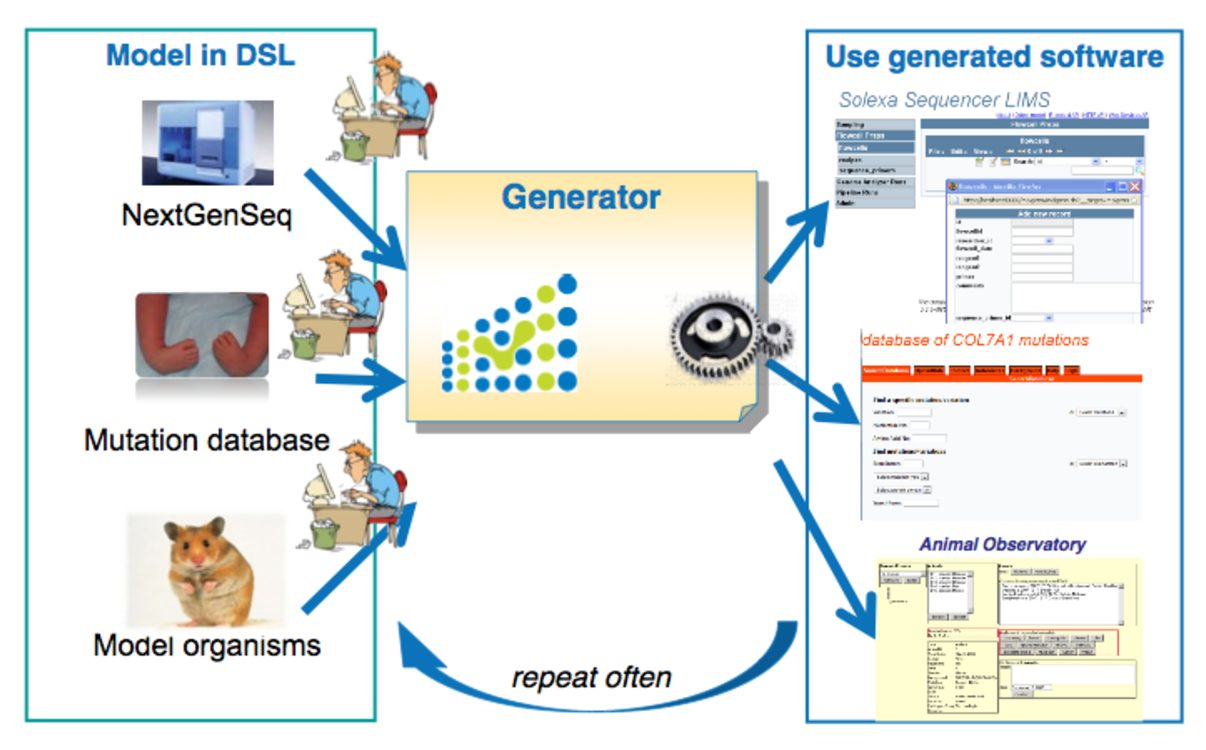
\includegraphics[width=0.9\textwidth]{eps/image_4_1.eps}
  \caption[CTLs.]{QTL and CTL analysis of two traits: a schematic of possible scenarios at a given marker. A trait can 
          have a QTL or no QTL at the given marker: there are four possible combinations in QTL analysis with two traits. 
          The trait pair can also have a CTL or no CTL and in the combined QTL and CTL analysis: the total number of possible 
          combinations is eight. Three additional scenarios refer to special cases when one trait or both traits are not 
          expressed in one genotype. For sake of simplicity it is assumed in this figure that there are two genotypes only, 
          e.g. as in a BC or RIL population. [We also ignore possible info on cis- and trans-mapping for the moment]}
          \label{fig:ctls}
  \end{figure}

  \subsection{QTL and CTL analysis of two traits}
  
  To describe the possible relationships between QTL and CTL we generate the possible scenario's as in figure \ref{fig:ctls}.\\
  {\bf(A)} The two traits have a QTL and a CTL at the given marker (1 scenario). This example shows the extreme scenario when the traits are 
  well correlated in one genotype and entirely uncorrelated in the other. The locus affects both the mean and the correlation. They could 
  have a regulatory factor in common, the effect of which is detected in QTL and CTL analysis.\\
  {\bf(B)} The two traits have a CTL at the given marker, but only one trait has a QTL at that marker (2 scenarios).  The locus affects the 
  correlation, and the mean of one trait only. They could have a regulator in common in which case the latter trait is downstream of the other 
  trait: this can happen e.g. if the locus leads to functionally different transcripts at equal expression levels for the trait without QTL, 
  and this effect is propagated to the trait with (therefore) a QTL.\\
  {\bf(C)} The two traits have a CTL but no QTL at the given marker (1 scenario). This example shows the extreme scenario when the traits 
  are well correlated in one genotype and entirely uncorrelated in the other.  The locus affects the correlation only. They could have a 
  regulatory factor in common, the effect of which is detected in CTL analysis only: e.g. if the locus leads to co-regulated transcription 
  in one genotype only.\\
  {\bf(D)} The two traits have no CTL at the given marker  (4 scenarios).  The locus does not change the correlation, it change the mean 
  if one or both traits have a QTL. The example shows the extreme scenario when both traits have a QTL but are entirely uncorrelated: they 
  could be downstream of the same or a different factor at the given region.\\
  {\bf(E)} The two traits have a CTL at the given marker, but the trait values are at the noise level in one genotype for one or both 
  traits (3 scenarios). This expression at noise level for one trait could result from e.g. hybridization failure for one genotype. One 
  or both traits can have a possibly artificial QTL and the two traits have a possibly artificial CTL. The example shows the scenario 
  when only one trait has a QTL.

\section{Inference of hierarchical relationship between traits}
  \subsection{Using information of co-localized CTL and QTL}
  Observing a significant CTL between T1 and T2 means that there is a factor (e.g. genetic regulator) located underneath 
  the CTL peak influencing the correlation between T1 and T2. This information of shared genetic control, therefore, 
  indicates that T1 and T2 are involved in the same biological pathway \cite{Tesson:2010}.

  The absence of QTL in trait T1 and the presence of QTL in trait T2 indicate that T2 is downstream of T1 in the 
  hierarchical network. The reasoning is that the variation caused by a genetic factor in T2 (QTL) has not 
  propagated to T1 \cite{Jansen:2009}. The reserve situation can also happen: Presence of QTL in trait T1 and the 
  absence of QTL in trait T2 indicate that T2 is upstream of T1 in the hierarchical network.

  The presence of QTL in both traits X and Y further confirms that T1 and T2 are related in the same pathway, and it 
  even allows us to go from inferring hierarchical relationship to causality using methods such as conditional 
  correlation \cite{Schadt:2007, Li:2010}.

  It should be noted that the co-localized CTL information does not exclude the existence of intermediate factor(s) 
  e.g. Z,  between T1 and T2 in the pathway, although the relative strength of correlation provides us 
  information on the distance among them in the network, e.g. higher correlation can indicate a shorter distance 
  between T1 and T2 in the network.\\

  \subsection{Using information of co-localized CTLs}
  When the CTLxy of X and Y co-localizes with CTLxz of X and Z and CTLyz of Y and Z, these three traits are possibly 
  involved in the same network. The relative effect sizes of these CTLs can be used to infer the order of X, Y and Z
  in the hierarchical network. For example, when CTLxy and CTLyz are larger than CTLxz, we can conclude that they 
  follow the order of X-Y-Z in the network, i.e. Y is in between of X and Z.

  Additionally when a QTL shows two or more co-localizing CTL we discovered a set of possible downstream targets 
  for the QTL. Which, when sample sizes permit, can be further annotated using gene ontology \cite{GeneOntology:2000} or 
  untangled by using methods like hierarchical inference (this paper) or causal inference \cite{Schadt:2005, Li:2006} 
  to obtain en even more detailed view of genetic regulation within the set.

  \subsection{Visualizing CTL information}
  Information obtained by CTL mapping can be visualized in several different ways the author found the most accessible 
  representation is a user-customizable network view. User customization helps researchers to add their own and/or 
  literature information to a network allowing for a rich interpretation of the created network. Network generated from 
  CTL mapping can be visualized by software tools including Cytoscape \cite{Cytoscape:2010, Cytoscape:2003}.

  CTL information allows us to draw lines from traits via markers to other traits reconstructing the underlying genetic 
  wiring. To create hierarchical networks we transforming the significant CTLs into network edges. This is done by 
  using a user defined genome wide FDR and then only transforming significant trait-marker-trait interactions into a 
  .sif network file.

\section{Cell type specific eQTL mapping in human GAWA data}
\label{sec:cellspecificeqtl}
  The number of available expression quantitative trait locus (eQTL) datasets from individual cell 
  types is limited because purifying cell types from mixtures is often challenging.  Since whole 
  peripheral blood is easily accessible and comprises many different cell-types, we developed 
  methodology to infer the specific cell-types in which eQTLs are operating,  alleviating the need 
  to sort cells and enabling interrogation of cell-types that are difficult to purify.

  We investigated whole peripheral blood of 5,683 unrelated individuals, and found that at least 
  8.5\% of all blood \emph{cis}-eQTLs are mediated by specific immune cell-types. Additionally, to our 
  knowledge, we present the first eQTL results for neutrophil granulocytes, a cell type that is 
  difficult to purify in the laboratory. We validated our findings in eQTL data of six purified 
  cell-types (lymphoblastoid cell-lines, B-cells, monocytes, CD4+ T-cells, CD8+ T-cells and 
  neutrophil granulocytes). Subsequent enrichment analysis of known disease-associated SNPs 
  revealed that Crohn's disease SNPs preferentially affect gene expression levels within neutrophil 
  granulocytes, underscoring the importance of neutrophils in Crohn's disease pathogenesis.

  \subsection{Background}
  In the past seven years, genome-wide association studies (GWAS) have identified thousands of genetic 
  variants that are associated with human disease\cite{Hindorff:2009}. The realization that many of 
  the disease-predisposing variants are noncoding, and that single nucleotide polymorphisms (SNPs) 
  often affect the expression of nearby genes (i.e. \emph{cis}-eQTLs) \cite{Powell:2012, Lude:2011, Zeller:2010}, 
  suggests these variants predominantly have a regulatory function. As such it is important to understand 
  in which specific tissues and cell-types these disease-associated variants exert their effect on disease.

  We have previously shown that whole peripheral blood is a suitable tissue to detect \emph{cis}-eQTL effects, 
  especially for SNPs that are associated with (auto) immune disorders \cite{Lude:2011, Westra:2013}. However, recent studies 
  suggest that disease-predisposing variants often exert their regulatory effect in a cell-type dependent 
  manner \cite{Brown:2013, Fairfax:2012, Fu:2012, Dimas:2009, Breitling:2008a}. This is problematic 
  when studying whole peripheral blood, since it is comprised out of   many different cell types that originate 
  from either the myeloid (e.g. neutrophil, granulocytes, monocytes) or lymphoid lineage (e.g. 
  B-cells or T-cells). An increase in the percentage of cells within one lineage decreases the 
  percentage of cells in the other (e.g. neutrophil percentage is strongly negatively correlated with 
  lymphocyte percentage; Supplementary Figure 1). Consequently, \emph{cis}-eQTLs that have been 
  detected in whole blood may actually reflect an effect within one single 
  cell-type, complicating the functional interpretation of disease predisposing variants. Although 
  several eQTL datasets have recently been presented on individual white blood cell types (for example, 
  monocytes\cite{Zeller:2010, Fairfax:2012} and T-cells \cite{Fairfax:2012, Ding:2010}), other white 
  blood cell types (particularly neutrophil granulocytes) are difficult to purify and culture in the lab 
  \cite{Grisham:1985}, even though they can reflect a substantial 
  proportion of circulating white blood cells (e.g. neutrophil granulocytes comprise approximately 62\% 
  of all peripheral blood mononuclear cells). In case eQTL datasets already exist for these individual 
  cell types, their sample-size is typically small, limiting statistical power to study the cell type 
  mediation of \emph{cis}-eQTLs in these cell types directly. As such, to our knowledge, we here present the 
  first eQTL analysis investigating neutrophil granulocytes.

  In this paper, we present a method that uses whole peripheral blood to infer in which cell-types these 
  eQTLs manifest themselves. We first estimate for each sample what the specific cell-type proportions 
  are (relying upon individual expression measurements of genes that serve as proxies for these cell-types) 
  and subsequently use a gene x environment interaction (G x E) model. This allows us to predict which 
  \emph{cis}-eQTLs are predominantly mediated by specific cell types in peripheral blood datasets that lack 
  any actual cell-count measurements. We apply our method to an unprecedented number of samples (5,683 
  unrelated whole peripheral blood samples from seven cohorts: EGCUT \cite{Metspalu:2004}, InCHIANTI 
  \cite{Tanaka:2009}, Rotterdam Study \cite{Hofman:2011}, Fehrmann \cite{Lude:2011}, SHIP-TREND 
  \cite{Teumer:2011}, KORA F4 \cite{Powell:2012, Mehta:2013}, and DILGOM \cite{Inouye:2010}). We 
  subsequently validate our predicted cell-type mediated eQTLs in six datasets of purified cell-types, and 
  observe that SNPs, associated with Crohn's disease are enriched for affecting gene expression levels in 
  neutrophil granulocytes.

  \begin{figure}[h!]
  \centering
  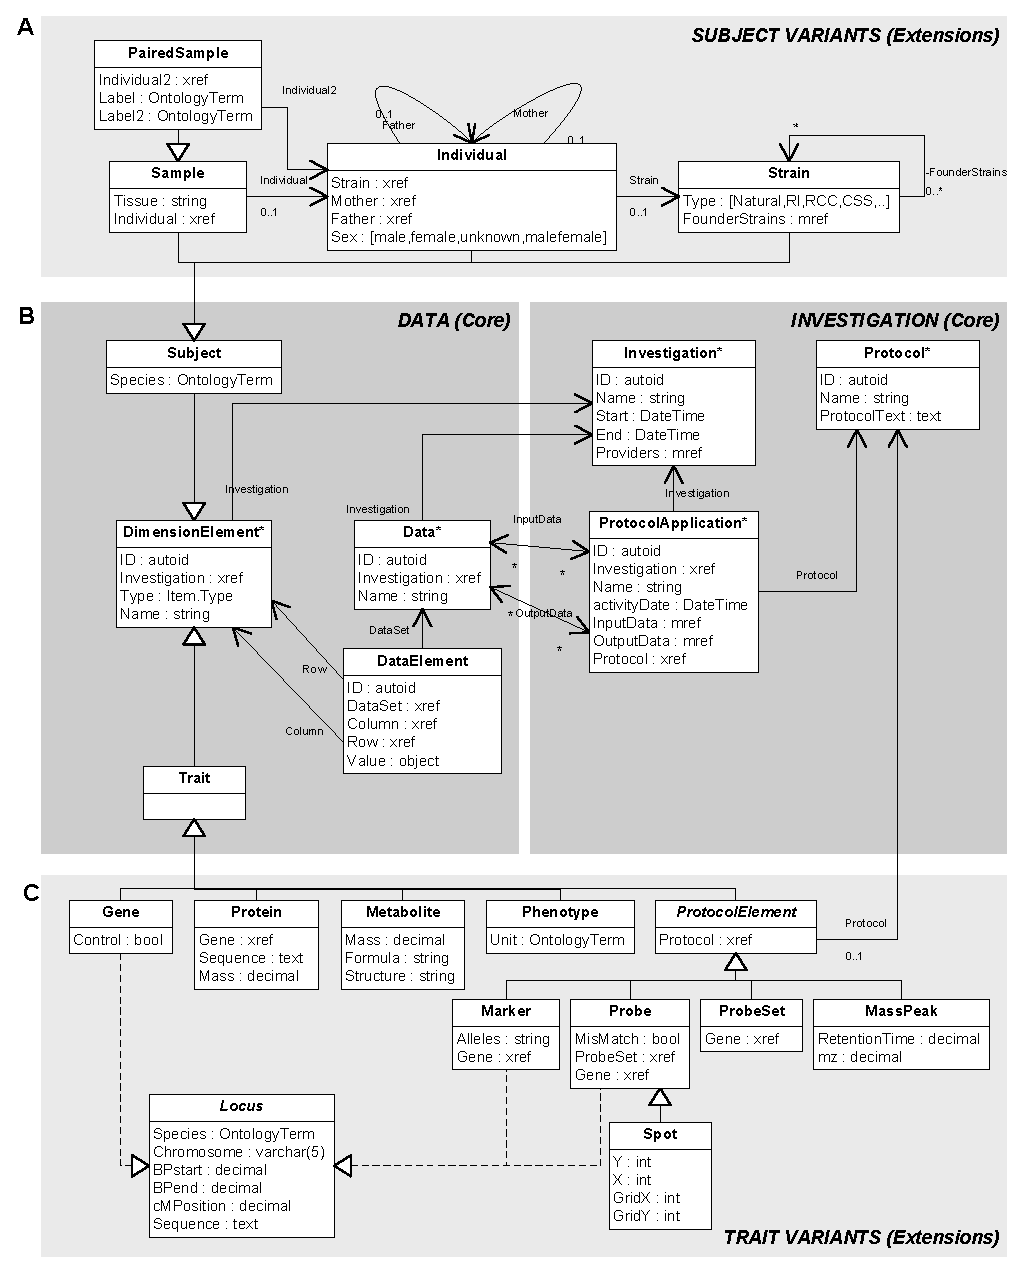
\includegraphics[width=0.9\textwidth]{eps/image_4_3.eps}
  \caption[Hematopoiesis overview]{Overview of cells involved in hematopoiesis. }
          \label{fig:fig4_3}
  \end{figure}

  \subsection{Results}
  Identification of cell-type specific eQTLs in mixtures (e.g. whole peripheral blood) is most easily 
  understood when assuming an extreme situation where in half of all blood samples the proportion of 
  e.g. neutrophil granulocytes is very low, and in the other half of all blood samples this proportion 
  is actually high. If an eQTL of interest is not showing any effect in the samples with a very low 
  neutrophil granulocyte proportion, while showing a strong effect in the samples with a high proportion, 
  this suggests the eQTL is specific for neutrophil granulocytes. In order to apply this reasoning on 
  a whole blood dataset, the neutrophil percentage of each sample should be known and is used as a 
  covariate in a linear model that includes an interaction term (cell type percentage x genotype). 
  We applied this strategy to 5,683 samples and determined which of the 13,124 \emph{cis}-eQTLs that we have 
  discovered before5 are mediated by individual cell-types. We concentrated on neutrophil granulocytes, 
  since 1) they are the most abundant immune cell type in whole blood, 2) to our knowledge no previous 
  eQTL studies in neutrophil granulocytes have been published before and 3) a strong inverse 
  relationship exists between the neutrophil granulocyte percentage and the lymphocyte percentage in 
  blood (Supplementary Figure 1): as such if one is studying neutrophil percentage, one automatically 
  investigates lymphocyte percentage as well.

  \begin{figure}[h!]
  \centering
  \includegraphics[width=0.9\textwidth]{eps/image_4_4.eps}
  \caption[Methods overview]{Overview of the method to detect cel type mediated eQTL effects. }
          \label{fig:fig4_4}
  \end{figure}

  However, neutrophil cell-count percentages were only available for the EGCUT and SHIP-TREND datasets. 
  To that end, we first developed a method that enabled us to approximate the cell type percentages for 
  datasets without cell type information (Figure \ref{fig:fig4_4}). We used the EGCUT cohort to identify a list of 58 
  Illumina HT12v3 probes that strongly positively correlated (Spearman's correlation coefficient > 0.55) 
  with neutrophil granulocyte counts. We then summarized the information of these 58 individual probes 
  into a single neutrophil granulocyte count estimate, by applying principal component analysis (PCA) 
  and using the first principal component. We validated the accuracy of this 58 probe neutrophil count 
  predictor, by applying this procedure to the SHIP-TREND cohort and correlating the estimated neutrophil 
  percentage to the actual neutrophil percentage. We observed a strong correlation (Spearman's correlation 
  coefficient = 0.82), indicating that these 58 probes jointly form a reliable proxy for neutrophil 
  percentage, and thus concluded we could use this procedure in the other cohorts as well.

  Every cohort determined the interaction model for 13,124 \emph{cis}-eQTLs, while using the neutrophil 
  percentage proxy x genotype as interaction term. We subsequently meta-analyzed the interaction 
  terms for each \emph{cis}-eQTL (up to 5,683 samples were tested per eQTL) and identified 1,117 \emph{cis}-eQTLs 
  with a significant interaction effect (8.5\% of all tested cis-eQTLs; FDR < 0.05; 1,037 unique SNPs 
  and 836 unique probes; Table 1, Supplementary Table 1). 909 (6.9\%) had a positive direction of 
  effect, which indicates that these \emph{cis}-eQTLs show stronger effect sizes in neutrophil granulocytes 
  (302 eQTLs, 283 unique SNPs and 244 unique probes after a more stringent Bonferroni correction). We 
  will refer to these as neutrophil mediated \emph{cis}-eQTLs. Another 208 (1.6\%) had a negative direction of 
  effect (20 eQTLs, 20 unique SNPs and 13 unique probes after a more stringent Bonferroni correction), 
  indicating a stronger \emph{cis}-eQTL effect size in lymphoid cells (since lymphocyte percentages are 
  negatively correlated with neutrophil percentages). We will refer to these 
  as lymphocyte mediated \emph{cis}-eQTLs. Overall, the directions of the significant interaction effects were 
  consistent across the different cohorts, indicating that our findings are robust. We did however observe 
  that a large sample-size is essential in order to find these 
  cell-type mediated \emph{cis}-eQTLs (Figure \ref{fig:fig4_5}): when studying fewer samples (ascertained by systematically 
  excluding more cohorts from our study) the number of significant cell-type mediated eQTLs decreases 
  quickly. This was particularly important for the lymphoid mediated \emph{cis}-eQTLs, since in blood, 
  myeloid cells are approximately twice as abundant as lymphoid cells, and consequently detection of 
  lymphoid mediated \emph{cis}-eQTLs is more challenging than detection of myeloid mediated \emph{cis}-eQTLs.

  We validated our findings in four purified cell-type gene expression datasets from the lymphoid 
  lineage (lymphoblastoid cell lines (LCLs), CD4+ T-Cells, CD8+ T-Cells and B-Cells; Figure \ref{fig:fig4_6}, 
  Supplementary Table 2) and two purified cell-type datasets from the myeloid lineage (monocytes and 
  neutrophil granulocytes). As expected, compared to \emph{cis}-eQTLs without a significant interaction term 
  (generic \emph{cis}-eQTLs) the 909 neutrophil mediated \emph{cis}-eQTLs and the 208 lymphoid mediated \emph{cis}-eQTLs 
  indeed showed very strong \emph{cis}-eQTL effects in the myeloid datasets (Wilcoxon P-value < 4.9 x 10-31) 
  and lymphoid datasets (Wilcoxon P-value < 7.8 x 10-14), respectively (Figure \ref{fig:fig4_6}). These results 
  indicate that our method is able to reliably predict whether a \emph{cis}-eQTL is mediated by a specific 
  cell type. We also assessed whether average gene expression levels within different cell-types might 
  be useful to predict whether a \emph{cis}-eQTL is mediated by a specific cell type, as it can be hypothesized 
  that if a certain gene is highly expressed within one single cell-type while it is only weakly 
  expressed in other cell-types, that the eQTL effect might manifest itself only in the highly expressed 
  cell-type. We indeed observed that, on average, the 909 neutrophil mediated and 208 lymphoid eQTL 
  genes showed slightly higher gene expression levels within the myeloid and lymphoid cell-types, 
  respectively (Supplementary Figure \ref{fig:fig4_6}). However, for many individual genes that showed a strong 
  cell-type mediated \emph{cis}-eQTL effect, the average expression levels within that cell-type were not 
  higher than the other blood cell-types. As such, it is not possible to predict whether an eQTL is 
  operating in a particular cell-type by solely assessing in which cell-type the gene expression level 
  of this eQTL gene is the highest.

  \begin{figure}[h!]
  \centering
  \includegraphics[width=0.9\textwidth]{eps/image_4_6.eps}
  \caption[Validation]{Validation in four purified cell-type gene expression datasets}
          \label{fig:fig4_6}
  \end{figure}

  We next assessed whether there are immune related diseases, for which the associated SNPs 
  preferentially have affect gene expression within neutrophils (i.e. are enriched for neutrophil 
  mediated \emph{cis}-eQTLs).  We concentrated on 2 immune related diseases for which at least 30 unique 
  genome-wide significant (P < 5 x 10-8) loci have been identified before (as reported in the Catalog 
  of Published Genome-Wide Association Studies19, accessed September 23, 2013). Per disease, we tested 
  whether the associated SNPs were enriched for neutrophil mediated \emph{cis}-eQTLs by using a binomial test. 
  To ensure we tested independent loci, we first pruned the SNPs for linkage disequilibrium (R2 > 0.2). 
  We observed significant enrichment (one-tailed P = 0.001, Table 2) for Crohn's disease. Out of 51 
  unique SNPs that showed a \emph{cis}-eQTL effect, 11 were neutrophil mediated. These 11 SNPs affect the 
  expression of 14 unique genes (ZGPAT, LIME1, SLC2A4RG, CISD1, IL18RAP, HOTAIRM1, NOD2, AC034220.3, 
  SLC22A4, PLCL1, CPEB4, LGALS9, RP11-514O12.4, RNASET2).

  \subsection{Discussion}
  Here we have shown that it is possible to infer in which cell-types \emph{cis}-eQTLs are operating, without 
  the actual need to sort cells. We used whole peripheral blood eQTL data of 5,683 unrelated samples. 
  By first estimating cell-type proportions and subsequent use of a G x E (i.e. the estimated cell-type 
  proportions) interaction model we were able to demonstrate that hundreds of \emph{cis}-eQTLs show stronger 
  effects in myeloid than lymphoid cell-types and vice versa. 

  Since we could subsequently replicate these results in 6 individual purified cell-type eQTL datasets 
  (two reflecting the myeloid and four reflecting the lymphoid lineage), this indicates G x E analyses 
  can provide important additional biological insights for many SNPs that have previously been found 
  to be associated with complex (molecular) traits. 

  However, two main criteria apply in order to identify such G x E effects: first, sample size should 
  be large. Although, to our knowledge, this is the largest eQTL study that has been conducted so-far 
  (5,683 samples), it is clear by sampling subsets of the participating cohorts (Figure 2), that more 
  G x E effects should be detectable with even larger sample sizes. Secondly, choosing the appropriate 
  environmental factor is essential in order to find convincing G x E effects: although we found 1,117 
  \emph{cis}-eQTLs that were mediated by myeloid or lymphoid cell-types, a recent G x E study that aimed to 
  detect \emph{cis}-eQTLs that were mediated by either gender or age (assessed in 5,254 samples) found only 
  five G x E effects that replicated in an independent cohort20. As such the choice of environmental 
  factor is crucial in order to find G x E interaction effects.

  Here, we have concentrated on identifying \emph{cis}-eQTLs that are preferentially operating in either 
  myeloid or lymphoid cell-types. We did not attempt to assess this for specialized cell-types within 
  the myeloid or lymphoid lineage. However, this is well possible if cell-counts are available for 
  these cell-types, or if these cell-counts can be estimated by using the expression levels of genes 
  that serve as proxies for those cell-counts. As such, identification of cell-type mediated eQTLs 
  for previously unstudied cell-types is possible, without the actual need to generate any new data. 
  However, it should be noted that these individual cell-types typically have a rather low abundance 
  within whole blood (e.g. natural killer cells only comprise ~2\% of all circulating white blood 
  cells). As a consequence, in order to have sufficient statistical power to identify eQTLs that are 
  mediated by these cell-types, very large whole blood eQTL sample-sizes are required (analogous to 
  the substantially lower number of identified lymphoid mediated \emph{cis}-eQTLs, as compared to the myeloid 
  mediated \emph{cis}-eQTLs, since neutrophils are twice as abundant as lymphoid cells in whole blood). 
  Additionally, such cell-types should show differences in abundance across different individuals, 
  rendering identification of \emph{cis}-eQTLs that are specific for certain cell-types impossible if those 
  cell-types have a near equal abundance in blood across each of the individuals.

  In order to improve statistical power to detect cell-type mediated eQTLs, we corrected the gene 
  expression for technical and batch effects (here we applied principal component analysis and removed 
  per cohort the 40 strongest principal components that affect gene expression). Such procedures are 
  commonly used when conducting \emph{cis}-eQTL mapping \cite{Lude:2011, Dubois:2010, Fu:2012, 
  Zhernakova:2013, Westra:2013, Lappalainen:2013}. Although this correction might diminish the 
  power to detect trans-eQTLs \cite{Westra:2013}, this concern does not apply to our G x E \emph{cis}-eQTL study: we first 
  determined the environment effect (i.e. neutrophil count percentage) for each individual samples by 
  combining the expression levels of 58 probes, based on the original expression data that was not 
  corrected for principal components. The subsequent G x E eQTL mapping was conducted on the expression 
  data that was corrected for principal components. Although for a specific G x E effect (e.g. a SNP 
  on chr. 6 in conjunction with neutrophil count percentage), the individual SNP or the individual 
  environmental factor might exert strong effects on overall blood gene expression levels (and thus 
  the SNP effect or the environmental factor effect might have been captured by any of the first 40 
  gene expression PCs), detection of the G x E effect will only become impossible when the specific 
  G x E effect (i.e. the specific combination of the SNP and environmental effect) would have been 
  captured by any of the first 40 gene expression PCs. We observed that the number of significantly 
  detected cell-type mediated \emph{cis}-eQTLs improved approximately two fold when correcting for these PCs, 
  without losing G x E effects that only had been detected in the uncorrected data (data not shown).

  We confined our analyses here to a subset of \emph{cis}-eQTLs for which we had previously identified a main 
  effect in whole peripheral blood \cite{Westra:2013}: for each \emph{cis}-eQTL gene, we here only studied the most 
  significantly associated SNP. Considering that for many \emph{cis}-eQTLs multiple, unlinked SNPs exist that 
  independently affect the gene expression levels, it is possible that we have missed myeloid or 
  lymphoid mediation of these secondary \emph{cis}-EQTLs.

  We anticipate that with the (pending) availability of large RNA-seq based eQTL datasets, statistical 
  power to identify cell-type mediated eQTLs will improve further: since RNA-seq enables very accurate 
  gene expression level quantitation and is not limited to a set of preselected probes that interrogate 
  well known genes (as is the case for microarrays), the detection of genes that can serve as reliable 
  proxies for individual cell-types will improve. Secondly, using RNA-seq data, it is possible to 
  assess whether SNPs that affect the expression of non-coding transcripts, affect splicing \cite{Lappalainen:2013} or result 
  in alternative polyadenylation \cite{Zhernakova:2013} are mediated by specific cell-types.

  Although we applied our method to whole blood gene expression data, our method can be applied to any 
  tissue, alleviating the need to sort cells or to perform laser capture micro dissection. The only 
  prerequisite is that eQTL data in such tissues is available for many samples. However, since an 
  increasing number of eQTL datasets in different tissues are now becoming available and eQTL meta-analyses 
  have proven successful \cite{Lude:2011, Westra:2013}, our approach provides a cost effective way to identify cell-type 
  mediated eQTLs, that is likely to reveal novel biological insight.



\chapter{High throughput infrastructure for system genetics}
\thispagestyle{empty}
\label{chap:xqtlwormbench}

\emph{Modern high-throughput technologies generate large amounts of genomic, transcriptomic, 
proteomic and metabolomic data, creating a major challenge in bioinformatics from the size 
of data collected and the multitude of technologies used. We present the xQTL workbench 
system \cite{Arends:2012}, a flexible and scalable platform to store and analyse all these 
new phenotype and genotype data using XGAP \cite{Swertz:2010a} dataformat and MOLGENIS software 
\cite{Swertz:2004}. We evaluated the system in multiple applications of which WormQTL database 
\cite{Snoek:2012} is presented here.}

\null
\vfill

\begin{myexampleblock}{Originally published as:}
  \authors{Morris A Swertz, Martijn Dijkstra, ..., Danny Arends, George Byelas, et al}\\
  \emph{The MOLGENIS toolkit: rapid prototyping of biosoftware at the push of a button}\\
  \bold{BMC Bioinformatics} (2010)\\\\

  \authors{Morris A Swertz, K Joeri v/d Velde, Bruno M Tesson, ..., Danny Arends, et al}\\
  \emph{XGAP: a uniform and extensible data model and software platform for genotype and phenotype experiments}\\
  \bold{Genome Biology} (2010)\\\\

  \authors{Danny Arends*, K. Joeri v/d Velde*, Pjotr Prins, Karl W. Broman, et al.}\\
  \emph{xQTL workbench: a scalable web environment for multi-level QTL analysis}\\
  \bold{Bioinformatics} (2012)\\\\

  \authors{Danny Arends*, L. Basten Snoek*, Joeri v/d Velde*, Yang Li*, et al.}\\
  \emph{WormQTL: Public archive and analysis web portal for natural variation data in Caenorhabditis spp}\\
  \bold{Nucleic Acids Research} (2012)
\end{myexampleblock}

\newpage

\begin{wrapfigure}{r}{0.5\textwidth}
  \centering
  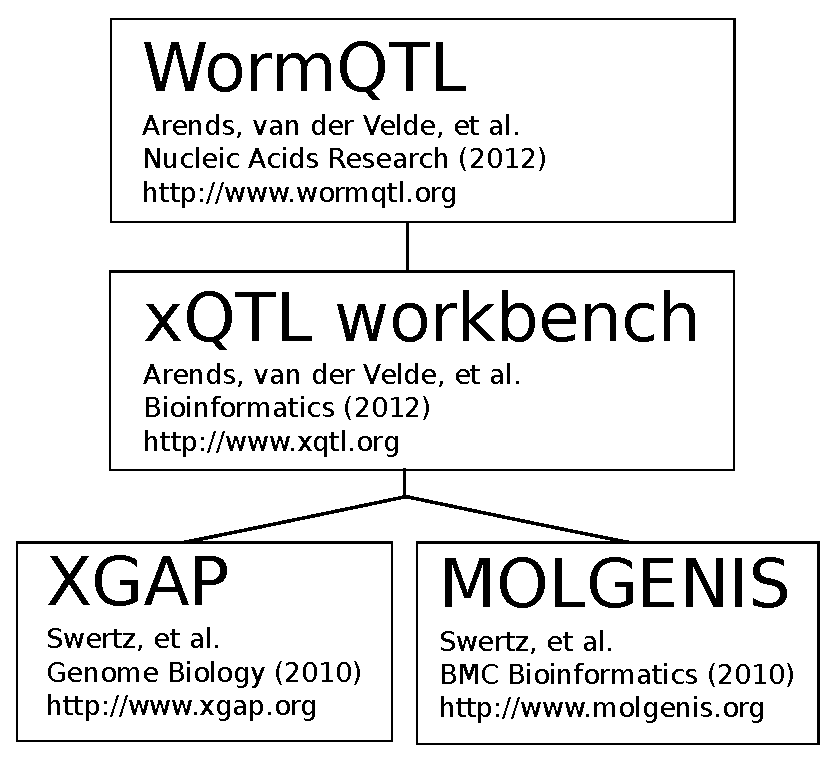
\includegraphics[width=0.4\textwidth]{eps/image_5_0.eps}
  \caption[Overview]
    {Overview of this chapter and how the different parts of this chapter are related to eachother.}
    \label{fig:Overview}
\end{wrapfigure}

Modern genetic and genomic technologies provide researchers with unprecedented amounts of raw and processed 
data and the need for software infrastructures to manage and process the large datasets produced is widely 
accepted \cite{Swertz:2004, Stein:2008, Thorisson:2009}. For example, recent genetical genomics 
\cite{Swertz:2004, Stein:2008, Thorisson:2009} studies have mapped gene expression (eQTL), 
protein abundance (pQTL) and metabolite abundance (mQTL) to genetic variation using genome-wide linkage and 
genome-wide association experiments on various microarray, mass spectrometry and proton nuclear magnetic 
resonance (NMR) platforms and in a wide range of organisms, including human \cite{Goring:2007, Tanaka:2009, 
Heap:2009}, yeast \cite{Brem:2002, Brem:2005}, mouse \cite{Bystrykh:2005}, rat \cite{Ramos:1999}, 
\emph{Caenorhabditis elegans} \cite{Li:2010} and \emph{Arabidopsis thaliana} \cite{Keurentjes:2006, Keurentjes:2007, Fu:2009}.

Understanding these and other high-tech genotype-to-phenotype data is challenging and depends on suitable 
'cyber infrastructure' to integrate and analyze data \cite{Stein:2008, Fay:2008}: data infrastructures to store and query the 
data from different organisms, biomolecular profiling technologies, analysis protocols and experimental 
designs; graphical user interfaces (GUIs) to submit, trace and retrieve these particular data; communicating 
infrastructure in, for example, R \cite{Ihaka:1996}, Java and web services to connect to different processing infrastructures 
for statistical analysis \cite{Alberts:2008, Fu:2007} and/or integration of background information from public 
databases \cite{Smedley:2008}; and a simple file format to load and exchange data within and between projects.

Many elements of the required cyber infrastructure are available: The Generic Model Organism Database (GMOD) 
community developed the Chado schema for sequence, expression and phenotype data \cite{Mungall:2007, OConnor:2008} and delivered reusable 
software components like gbrowse \cite{Stein:2002}; the BioConductor community has produced many analysis packages that 
include data structures for particular profiling technologies and experimental protocols \cite{Gentleman:2004}. 

Some integrated cyber infrastructures are also available: the National Center for Biotechnology Information (NCBI) 
has launched dbGaP (database of genotypes and phenotypes) \cite{Mailman:2007}, a public database to archive genotype 
and clinical phenotype data from human studies; and the Complex Trait Consortium has launched GeneNetwork \cite{GeneNetwork:2004}, 
a database for mouse genotype, classical phenotype and gene expression phenotype data with tools for 'per-trait' quantitative trait loci (QTL) analysis.

However, a suitable and customizable integration of these elements to support high throughput genotype-to-phenotype 
experiments is still needed \cite{Thorisson:2009}: dbGaP, GeneNetwork and the model organism databases are designed 
as international repositories and not to serve as general data infrastructure for individual projects; many of the 
existing bespoke data models are too complicated and specialized, hard to integrate between profiling technologies, 
or lack software support to easily connect to new analysis tools; and customization of the existing infrastructures 
dbGaP, GeneNetwork or other international repositories \cite{Zeng:2007, Hu:2007} or assembly of Bioconductor and 
generic model organism database components to suit particular experimental designs, organisms and biotechnologies 
still requires many minor and sometimes major manual changes in the software code that go beyond what individual 
lab bioinformaticians can or should do, and result in duplicated efforts between labs if attempted. Existing open 
source web-based tools for QTL analysis, such as webQTL \cite{Chesler:2004} and QTLNetwork \cite{Yang:2008}, are 
not easily extendable to different settings and computationally scalable for whole genome analyses.

We here present xQTL workbench and its application in the WormQTL database. WormQTL (http://www.wormqtl.org) is an 
easily accessible database enabling search, comparative analysis and meta-analysis of all data on variation in \emph{Caenorhabditis spp}.
All was built on top of xQTL workbench, a generic scalable web platform for the mapping of quantitative trait loci (QTLs)
 at multiple levels: for example gene expression (eQTL), protein abundance (pQTL), metabolite abundance (mQTL) and phenotype 
(phQTL) data. xQTL workbench supports storing of raw, intermediate and final result data, and analysis protocols and history 
for reproducibility and data provenance using XGAP data model \cite{Swertz:2010a}. Use of Molgenis \cite{Swertz:2010b} helped 
to build and customize the software. All is conveniently accessible via standard Internet browsers on Windows, Linux or Mac 
(and using Java, R for the server). xQTL workbench, MOLGENIS, XGAP and WormQTL are related to eachother as outlined in 
Figure \ref{fig:Overview}, and.are described in detail below.

\section{High throughput data analysis (xQTL workbench)}
Existing open source web-based tools for QTL analysis, such as webQTL \cite{Wang:2003, Chesler:2004} and 
QTLNetwork \cite{Yang:2008}, are not easily extendable to different settings and computationally 
scalable for whole genome analyses. \xqtlwb makes it easy to analyse large and complex 
datasets using state-of-the-art QTL mapping tools and to apply these methods to millions of 
phenotypes using parallelized 'Big Data' solutions \cite{Trelles:2011}.
\xqtlwb also supports storing of raw, intermediate and final result data, and analysis protocols 
and history for reproducibility and data provenance. Use of MOLGENIS\cite{Swertz:2010b} 
helps to customize the software. All is conveniently accessible via standard Internet browsers on 
Windows, Linux or Mac (and using Java, R for the server).

xQTL workbench is a scalable web platform for the mapping of quantitative trait loci (QTLs) 
at multiple levels: for example gene expression (eQTL), protein abundance (pQTL), metabolite 
abundance (mQTL) and phenotype (phQTL) data. Popular QTL mapping methods for model organism 
and human populations are accessible via the web user interface. Large calculations scale 
easily on to multi-core computers, clusters and Cloud. All data involved can be uploaded 
and queried online: markers, genotypes, microarrays, NGS, LC-MS, GC-MS, NMR, etc. When new 
data types come available, xQTL workbench is quickly customized using the MOLGENIS software 
generator. xQTL workbench provides visualization of QTL profiles, single and multiple QTL 
mapping methods, easy addition of new QTL analyses, scalable data management and analysis 
tracking, described below:

\subsection{Features}
\xqtlwb provides visualization of QTL profiles, single and multiple QTL mapping methods, easy addition 
of new QTL analyses, scalable data management and analysis tracking.

\begin{figure}[h!]
  \centering
  \includegraphics[width=0.75\textwidth]{eps/image_5_4.eps}
  \caption[xQTL workbench.]{Screenshot of xQTL workbench with all features enabled, (1) Import phenotype, genotype 
          and genetic map data, examples are given per import type; (2) Search through the whole database, explore 
          and browse your data using MOLGENIS generated web-interfaces; (3) Run R/qtl QTL mapping, the general 
          plugin allows users to perform not only QTL mapping but also other analyses; (4) Use default (or custom) 
          plugins to explore results (e.g. Heatmaps, QTL profiles); (5) Add new tools to the workbench (for 
          Bioinformaticians); (6) User management and access control of the system (Only for admins); (7) Expert 
          settings can be altered in the admin tab (Only for admins); (8) Connect/share data using generated API's 
          to R statistics, REST/JSON, SOAP.}
          \label{fig:xQTLworkbench}
\end{figure}

\begin{enumerate}\itemsep1pt
\item \emph{Explore QTL profiles} - Through the web-interface, users can explore mapped QTLs, and 
underlying information by viewing QTL plots in an interactive scrollable and zoomable window. 
\xqtlwb has support for other common image formats, such as PNG, JPG, SVG and embedded postscript; 
useful for publishing scientific results online, and on paper. From the output, main database identifiers, 
such as gene, protein and/or metabolite identifiers are automatically linked-out to matching external 
web pages of public database such as NCBI, KEGG, and Wormbase.
\item \emph{Single and multiple QTL mapping} - \xqtlwb wraps R/qtl \cite{Broman:2003, Arends:2010} in a 
web-based analysis framework offering all important QTL mapping routines, such as the EM algorithm, 
imputation, Haley-Knott regression, the extended Haley-Knott method, marker regression, and Multiple 
QTL mapping. In addition, \xqtlwb includes R/qtlbim, a library which provides a Bayesian model 
selection approach for mapping multiple interacting QTL \cite{Yandell:2007} and Plink, a library for 
association QTL mapping on Single Nucleotide Polymorphisms (SNP) in natural populations \cite{Purcell:2007}.
\item \emph{Add new analysis tools} - \xqtlwb supports flexible adding of more QTL analysis software: 
any R-based, or command-line tool, can be plugged in. All analysis results are uploaded, stored and 
tracked, in the \xqtlwb database through an R-API. When new tools are added, they can build on the 
high-level multi-core computer, cluster and Cloud management functions, based on TORQUE/OpenPBS and 
BioNode \cite{Prins:2012}. \xqtlwb can be made part of a larger analysis pipeline using interfaces to R, 
Excel, REST and SOAP web services and Galaxy \cite{Goecks:2010}.
\item \emph{Track and trace} - When a new analysis protocol or R script is defined, this protocol 
can easily be applied to new data. Also, \xqtlwb keeps track of history. Re-use of analysis protocols 
can be done in an automated fashion. Previous analyses can be rerun without resetting parameters. 
\xqtlwb provides an online overview of past analyses e.g. which analyses were performed, by who, when 
and display settings applied.
\item \emph{Scalable data management} - \xqtlwb has a consistency checking database based on XGAP 
specification \cite{Swertz:2010a}, user interfaces to manage and query genotype and phenotype data 
sets, and support for various database back-ends including HSQL (standalone) and MySQL. Phenotype, 
genotype and genetic map data can be imported as text (TXT), comma separated (CSV), and Excel files. 
\xqtlwb handles and stores large data in a new and efficient binary edition of the XGAP format, named 
XGAPbin (extension .xbin), documented online. Such binary formats are essential when handling, storing 
and transporting multi-Gigabyte datasets.
\item \emph{Customize to research needs} - Additional modules for new data modalities can be added using 
MOLGENIS software generator \cite{Swertz:2010b}. The 'look and feel' of \xqtlwb is adaptable to 
institute or consortium style by changing a simple template which is described in the \xqtlwb 
documentation enabling seamless integration into an existing web-site or intranet site, such as 
recently for EU-PANACEA model organism project and LifeLines biobank.
\end{enumerate}

\subsection{Reusable software (MOLGENIS)}
xQTL workbench was implemented using MOLGENIS. MOLGENIS was born from the observation that bioinformaticians 
are under continuous pressure to both tackle the complexity and diversity of new biological systems and 
analytical methods and to translate these quickly into flexible informatics infrastructures, while keeping 
up with the unpredictable evolution of molecular biotechnologies and the increasing scale of experiments.

While standardization of tools and data formats in open source projects like the Generic Model Organism 
Database, GMOD \cite{OConnor:2008}, and the Open Bioinformatics Foundation, OBF \cite{OBF:2010:Online}, have 
been indispensable in reducing the development efforts needed via reusable and easy to integrate components, 
new research must also be quickly accommodated, for which efficient software variation mechanisms are needed.

Figure \ref{fig:modelDrivenDevelopment} outlines the 'model-driven' development method that several 
bioinformatics projects adopted in recent years to enable fast and flexible infrastructure development. 
We demonstrate step-by-step how bioinformaticians can use a domain-specific language to efficiently model 
the biological details of their particular biological system, and use MOLGENIS software generation tools to 
automatically generate a web application tailored to the experiments of their biologists, building on reusable components. 

Next, we evaluate the results of these methods in the development of a range of MOLGENIS applications 
\cite{Swertz:2004, Swertz:2010a, Thorisson:2009, Leu:2010, Li:2009, Smedley:2008}, that is, software 
applications generated using the MOLGENIS toolkit. We found up to 30 times efficiency improvement compared 
to hand-writing software, while providing a richness of features practically unfeasible to produce by 
hand but not yet provided by related projects. We conclude by inviting the bioinformatics community to 
add more MOLGENIS models, components and generators to quickly generate all the software infrastructures biologists want to have.

\begin{figure}[ht!]
  \centering
  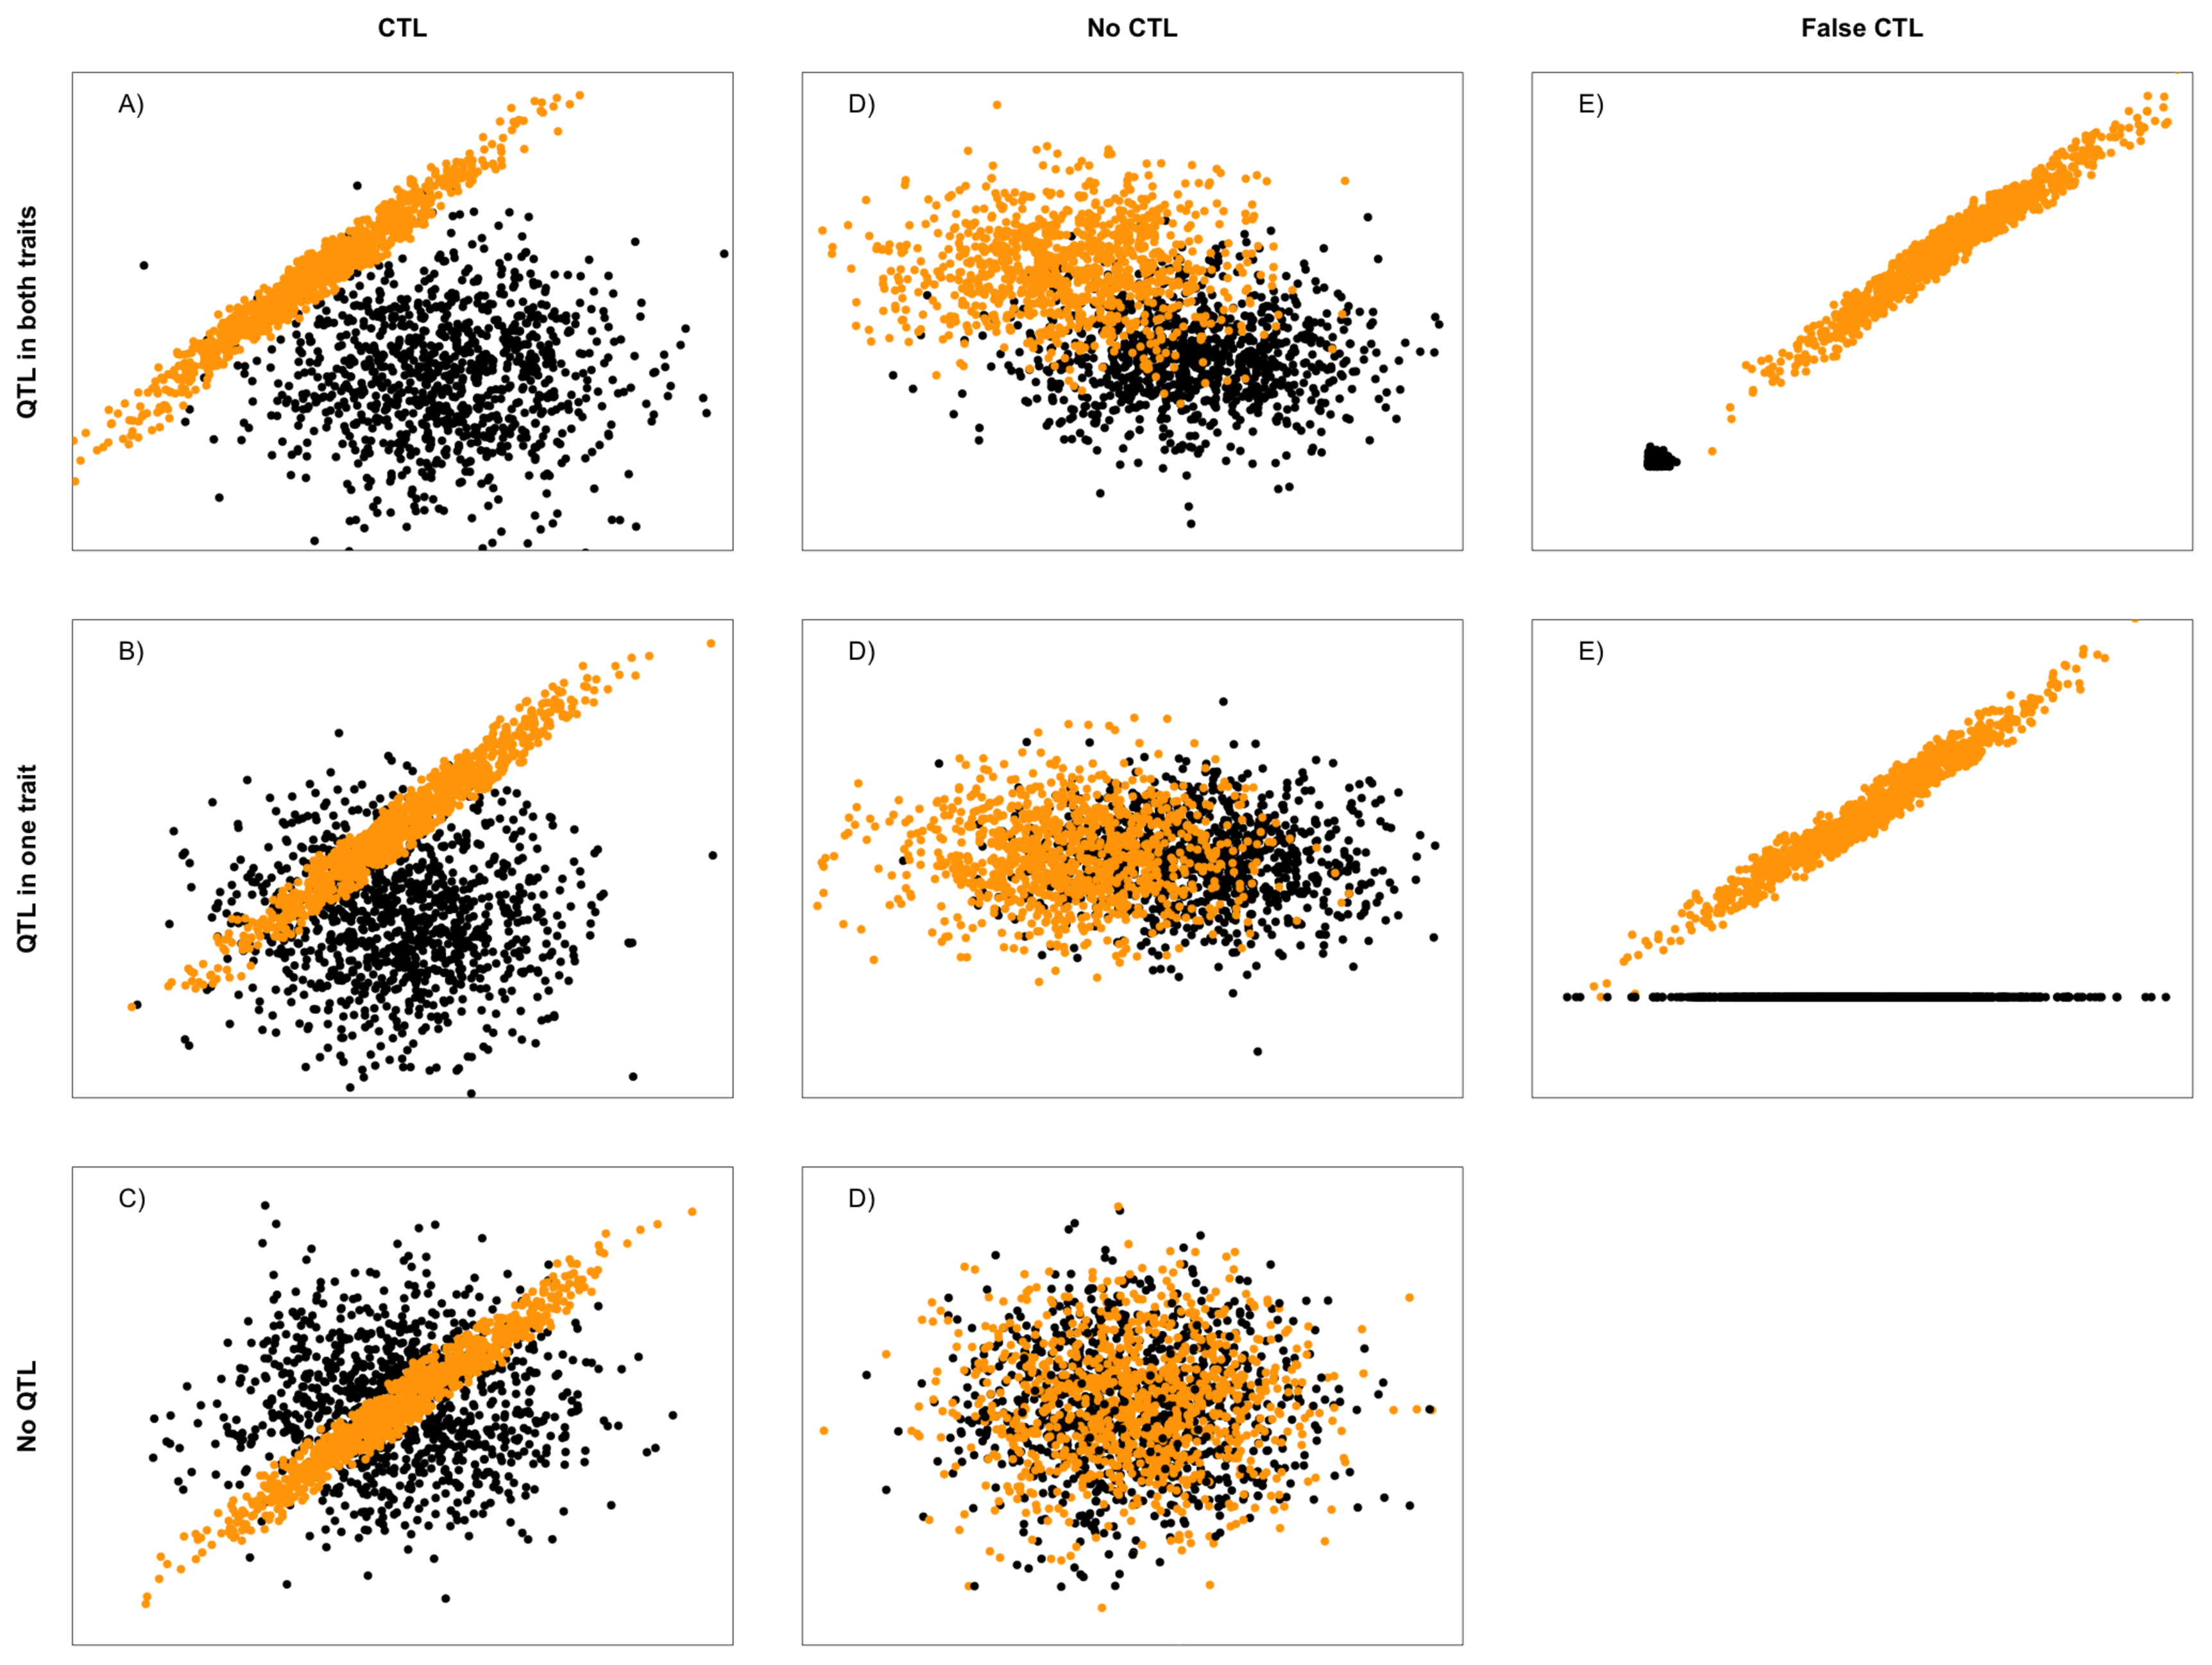
\includegraphics[width=0.9\textwidth]{eps/image_5_1.eps}
  \caption[MOLGENIS]
    {Many minor and major changes have to be written in software code before a 'standard' software infrastructure 
    accommodates a particular research. Using 'model-driven' development methods a bioinformatician only need to 
    model what is needed for his experiment using a therefore optimized domain specific language (DSL). Generators 
    quickly produce all the software logic to compose a full software infrastructure that accommodates these needs. 
    When experimental needs change, a bioinformatician can (re)run the same generator with an adapted model file 
    to quickly produce another variant of software infrastructure. This vastly reduces 'time-to-research' and 
    enables bioinformaticians to quickly develop a suite of software infrastructures, with each variant accommodating 
    a specific research task, while still on track to reuse, integrate and share the best standard features with 
    other labs and bioinformaticians.}
    \label{fig:modelDrivenDevelopment}
\end{figure}

The MOLGENIS toolkit is based on the method of model-driven development which emerged in the 1990s 
from the computer industry. Below we discuss the MOLGENIS' modeling language, the generators and 
reusable components. 

\subsubsection{Modeling language}
A custom MOLGENIS application can be defined in a single file. The file is written in MOLGENIS' 
modeling language. One can think of MOLGENIS' modeling language as a 'domain-specific language' 
\cite{Deursen:2002}, in this case to compose biosoftware infrastructures. The level of abstraction 
is raised, so no lengthy, technical or redundant details on how each feature should be implemented 
in general programming languages have to be given.

In most cases, knowledge of the DSL is all that is needed to produce a custom MOLGENIS application 
variant. The domain-specific language was implemented using XML so that model files can be edited 
using off-the-shelf XML editors. However, you may want to include hand-programmed components into 
a particular MOLGENIS instance. For example, for the eXtensible Genotype And Phenotype (XGAP) 
database application of MOLGENIS \cite{Swertz:2010a}, we developed a 'MatrixViewer' that builds on the generated 
components, which saved us the work of writing the plug-in from scratch. This requires a model 
sentence that points to the 'plug-in' (allowing it to be seamlessly integrated) as well as 
hand-programming of the plug-in itself.

\subsubsection{Reusable components}
Each MOLGENIS application follows the widely accepted three-layered architecture design of web 
applications. MOLGENIS' reusable components provide building blocks with a modular structure, which 
allows them to be assembled in diverse combinations, similar to prefabricated houses that are built 
from modular walls instead of bricks. Some building blocks are semi-finished and need to be 
'completed' before use (which is automated in MOLGENIS via the generators and inheritance). We based 
the design of MOLGENIS on industry-proven design patterns from the 'patterns for enterprise 
application architecture' (PEAA), a catalog of proven solutions for software design problems 
that we used as a guideline \cite{Fowler:2002}. The logic of the reusable components is implemented using 
Java (\url{http://java.sun.com/}); the HTML layout for the user interface is encoded in Freemarker 
templates (\url{http://freemarker.sourceforge.net/}); and the database back-end using MySQL, PostgreSQL 
or HSQLDB.

\begin{figure}[h!]
  \centering
  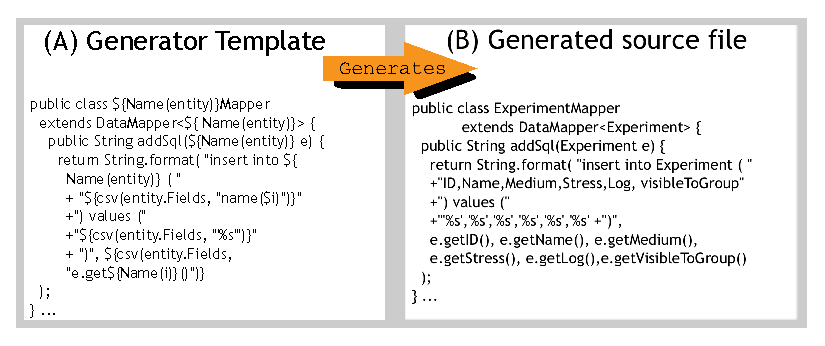
\includegraphics[width=1.0\textwidth]{eps/image_5_2.eps}
  \caption[Templates]
    {MOLGENIS generators are implemented as templates. This example shows the generator for a database component 
    (A). This template is applied to each <entity> in the model to generate many complete DataMappers that would 
    otherwise need to be written by hand. (B) shows an example of the generated source files, in this case for 
    <entity name="Experiment"> as described in Figure 1. The command \$Name(entity) translates to the name of the 
    entity ("Experiment") and command \${csv(\$entity.Fields, x)} means that command 'x' is applied to each field 
    of the entity and returned as a comma separated string (csv).}
	\label{fig:Generators}
\end{figure}

\subsubsection{Generators}
The generators are compact specifications of how each database feature should be implemented. 
The MOLGENIS toolkit now has over 20 generators, but normal users will never need to take a look 
inside. However, for readers wanting to create their own generators, figure \ref{fig:Generators} provides an example 
of the simple, text-based, generators we use. Each generator consists of two files: a Freemarker 
template that describes the code to be generated (similar to that shown in figure \ref{fig:Generators}a) and a Java 
'Generator' class that controls the generating process. A new generator can be developed as 
follows: First write some examples of the desired programs by hand, where possible using similar 
patterns and mark which parts are variable between them. Then copy one of these examples into 
a generator template (text file) and replace all variable parts with 'holes' that 
are to be filled by the code generator based on parameters from DSL. At each generation, the 
template is then automatically copied and the 'holes' filled, based on parameters described in 
the domain-specific language, saving much laborious manual work. 

\subsubsection{Results}
To start generating your own MOLGENIS application, you can download a ready-to-use 'workspace' 
from \url{http://www.molgenis.org/}, which can be edited using the commonly used Eclipse integrated 
development environment (IDE) tool (\url{http://www.eclipse.org/}). Extensive manuals are available to 
help install the Java, MySQL, Tomcat and Eclipse software needed and to learn how to walk through 
the Eclipse workspace to edit models and generate and run MOLGENIS instances; most new users can 
complete this part in about three hours. Detailed examples on how these features can be 
used to support actual microarray or genetical genomics experiments can be found in \cite{Swertz:2010a, Li:2009, Smedley:2008}.

After completing a MOLGENIS model and running the generator as described above, you have a 
ready-to-use software application. The features you get when running the generated result as 
a web application: a fully functional system where researchers can upload, manage, browse 
and query their biological data that conform to the model, optionally enhanced with analysis 
tools to explore and annotate (depending on the plug-ins).

An important feature is human readable and printable documentation of your model, including a graphical 
overview showing relationships in UML which is of great use when still designing and discussing the model 
in a team. The next step is typically using the web user interface to populate and test your application 
with real data. To enable batch loading from a spreadsheet application such as Excel, the system comes with 
a tab-delimited import/export tool tailored for your data which you can use from the user interface as well 
as via a command-line tool; i.e., the headers of your Excel file have to match the fields you have defined 
in the model, In our experience, most computational biologists greatly appreciate the use of the R interface 
to load, analyze and re-store data from within the R statistical environment with web services to connect 
to workflow tools. Finally, advanced programmers may want to customize the layout or integrate their own 
scripts into the user interface, that is, create plug-ins that are seamlessly integrated with the generated 
software. Typical examples here are the integration of R scripts that produce graphical overviews of the data, 
enabling them to be run by non-technical research colleagues

\subsubsection{Applications of MOLGENIS}
Since the earliest MOLGENIS application \cite{Swertz:2004}, we have successfully evaluated use of 
the MOLGENIS toolkit to build a wide range of biomedical applications \cite{Swertz:2010a, Fredman:2002, 
Leu:2010, Li:2009, Smedley:2008}, ranging from sequencing to proteomics.A full list MOLGENIS applications 
can be found at \url{http://www.molgenis.org/}. Each of these MOLGENIS projects reported major benefits 
from the short cycle from model to running system to enable quick evaluation (500 lines of model XML 
replaces 15,000 lines of programming code) and use of the batch loading of data to evaluate how the newly 
built system works with real data. More often than not, MOLGENIS helped in finding inconsistencies in 
existing data that would otherwise have gone unnoticed, leading to experimental errors. In our experience, 
a typical MOLGENIS generator run gives you about 90\% of the application that is desired 'for free', with the 
remaining 10\% typically filled in using plug-ins that are written by hand. The MOLGENIS toolkit has also 
been used to extend or replace existing software applications: the ExtractModel tool allows you to generate 
a MOLGENIS application from an existing database, which can then be run side-by-side with code developed 
previously, providing the best of both generated and hand-written worlds.

\subsection{Extensible Genotype and Phentype data (XGAP)}
We present an extensible software model for the genotype and phenotype community, XGAP. Readers 
can download XGAP (\url{http://www.xgap.org/}) or auto-generate a custom version using 
MOLGENIS with programming interfaces to R-software and web-services or user interfaces for 
biologists. XGAP has simple load formats for any type of genotype, epigenotype, transcript, 
protein, metabolite or other phenotype data. Current functionality includes tools ranging 
from eQTL analysis in mouse to genome-wide association studies in humans.

\subsubsection{XGAP - A minimal and extensible object model}
Another foundation of xQTL workbench was the development of an extensible data model for genotype 
and phenotype experiments (XGAP) that is designed as a platform to exchange data and tools and 
to be easily customized into variants to suit local experimental models.

Use of software domain specific language and auto-generation, implemented using MOLGENIS, aims to ease 
and speed up customization/variation into new XGAP versions for new biotechnologies and alternative 
experimental designs while ensuring consistent programming interfaces for the integration and sharing 
of existing analysis tools. Standardized extension mechanisms should balance between format/interface 
stability for existing data types and tools, and flexibility to adopt new ones.

We developed the XGAP object model to uniformly capture the wide variety of (future) genotype and phenotype data, building 
on generic standard model FuGE (Functional Genomics Experiment) \cite{Jones:2007} for describing 
the experimental 'metadata' on samples, protocols and experimental variables of functional genomics 
experiments, the OBO model (of the Open Biological and Biomedical Ontologies foundry for use of 
standard and controlled vocabularies and ontologies that ease integration \cite{Smith:2007}, 
and lessons learned from previous, profiling technology-specific modeling efforts \cite{Brazma:2006}.

Figure \ref{fig:XGAP}b shows the core components of a genotype-to-phenotype investigation: the biological 
subjects studied (for example, human individuals, mouse strains, plant tissue samples), the 
bio molecular protocols used (for example, Affymetrix, Illumina, Qiagen, liquid 
chromatography/mass spectrometry (LC/MS), Orbitrap, NMR), the trait data generated (usually 
data matrices with, for example, phenotype or transcript abundance data), the additional 
information on these traits (for example, genome location of a transcript, masses of LC/MS peaks), 
the wet-lab or computational protocols used (for example, MetaNetwork \cite{Fu:2007} in the case of QTL and
network analysis) and the derived data (for example, QTL likelihood curves).

\begin{figure}[ht!]
  \centering
  \includegraphics[width=0.75\textwidth]{eps/image_5_3.eps}
  \caption[XGAP.]
    {Experimental genotype and (molecular) phenotype data can be described using Subject, Trait, Data and DataElement; 
    the experimental procedures used can be described using Investigation, Protocol and ProtocolApplication (B). Specific 
    attributes and relationships can be added by extending core data types, e.g. Sample and Gene (A,C). The model is 
    described in UML: Arrows denote relationships (Data has a field Investigation that refers to Investigation ID); 
    Triangled lines denote inheritance (Metabolite inherits all properties ID, Name, Type from Trait, next to mass, 
    formula and structure); Triangled dotted lines denote use of interface (Spot 'implements' properties of Locus); 
    relationships are shown both as arrows and as properties ('xref' for one-to-many , 'mref' for many-to-many 
    relationships). Asterisk* marks FuGE derived types.}
    \label{fig:XGAP}
\end{figure}

We describe these biological components using FuGE data types and XGAP extensions thereof. 
Investigation binds all details of an investigation. Each investigation may apply a series 
of bio molecular \cite{Brown:2005} and computational \cite{Carey:2007,Alberts:2008,Fu:2007,Bhave:2007} 
Protocols. The applications of such Protocols are termed ProtocolApplications, which in the case 
of computational Protocols may require input Data and will deliver output Data.These data have the 
form of matrices, the DataElements of which have a row and a column index. Each row and column refers to a DimensionElement, 
being a particular Subject or a particular Trait. 

Figure \ref{fig:XGAP}a and \ref{fig:XGAP}c shows how the XGAP model can be extended to accommodate details on 
particular types of subjects and traits in a uniform way. A Trait can be a classical phenotype 
(for example, flowering - the flowering time is stored in the DataElement) or a bio molecular 
phenotype (for example, Gene X it's transcript abundance is stored in the DataElement). A 
Trait can also be a genotype (for example, Marker Y is a genomic feature observation that is 
stored in the DataElement). 

Genomic traits such as Gene, Marker and Probe all need additional information about their genome 
Locus to be provided. Similarly, a Subject can be a single Sample (for example, a labeled 
biomaterial as put on a microarray) and such a sample may originate from one particular Individual. 
It may also be a PairedSample when biomaterials come from two individuals - for example, if 
biomaterial has been pooled as in two-color microarrays. An individual belongs to a particular 
Strain. When new experiments are added new variants of Trait and Subject can be added in a similar 
way.

Several standard data types were also inherited from FuGE to enable researchers to provide 
'Minimum Information' for QTLs and Association Studies such as defined in the MIQAS checklist 
 - a member of the Minimum Information for Biological and Biomedical Investigations (MIBBI) 
guideline effort \cite{Taylor:2008}

\subsubsection{Simple text-file format for data exchange}
To enable data exchange using the XGAP model, we produced a simple text-file format (XGAP-TAB) based 
on the experience that for data formats to be used, data files should be easily created using simple 
Excel and text editor tools and closely resemble existing practices. This format is automatically 
derived from the model by requiring that all annotations on Investigations, Protocols,Traits, Subjects, 
and extensions thereof, are described as delimited text files (one file per data type) with columns 
matching the properties described in the object model and each row describing one data instance. 
Optionally, sets of DataElements can also be formatted as separate text matrices with row and column 
names matching these in the Trait and Subject annotation files, and with each matrix value matching 
one DataElement. The dimensions of each data matrix are then listed by a row in the annotations on Data.


\subsubsection{Application programming interfaces}
De facto standard analysis tools are emerging, for example, tools for transcript data [20,21,24] or 
metabolite abundance data [22] to mention just a few. These tools are typically implemented using the 
open source software for statistical analysis and graphics named R \cite{Ihaka:1996}. 

Bioinformaticians can connect their particular R or Java programs to the XGAP database using an API 
with similar functionality to the GUI, that is, using simple commands like 'find', 'add' and 'update' 
(R/API, Java/API). Scripts in other programming languages and workflow tools like Taverna \cite{Oinn:2004} can 
use web services (SOAP/API) or a simple hyperlink-based interface (HTTP/API). On top of this, conversion 
tools have been added to the R interface to read and write XGAP data to the widely used R/qtl package \cite{Broman:2003, Arends:2010}.

Based on these experiences, we expect use of XGAP to help the community of genome-to-phenome 
researchers to share data and tools, notwithstanding large variations in their research aims. 

The XGAP data format can be used to represent and exchange all raw, intermediate and result 
data associated with an investigation, and an XGAP database, for instance, can be used as a 
platform to share both data and computational protocols (for example, written in the R 
statistical language) associated with a research publication in an open format. We envision 
a directory service to which XGAP users can publish metadata on their investigations either 
manually or automatically by configuring this option in the XGAP administration user interface. 
This directory service can then be used as an entry point for federated querying between the 
community of XGAPs to share data and tools. Groups that already have an infrastructure can 
assimilate XGAP to ease evolution of their existing software.

Next to their existing user tools, they can 'rewire' algorithms and visual tools to also use 
the MOLGENIS APIs as data backend. Thus, researchers still have the same features as before, 
plus the features provided by the generated infrastructure (for example, data management GUIs, 
R/API) and connected tools (for example, R packages developed elsewhere). Moreover, much 
less software code needs to be maintained by hand when replacing hand-written parts by 
MOLGENIS-generated parts,  allowing software engineers to add new features for researchers 
much more rapidly. We invite the broader community to join our efforts at the public XGAP.org 
wiki, mailing list and source code versioning system to evolve and share the best XGAP 
customizations and GUI/API 'plug-in' enhancements, to support the growing range of profiling 
technologies, create data pipelines between repositories, and to push developments in the 
directions that will most benefit research.

\section{A worm database (WormQTL)}
Here, we present an application of \xqtlwb: WormQTL (http://www.wormqtl.org), an 
easily accessible database enabling search, comparative analysis and meta-analysis of all 
data on variation in \emph{Caenorhabditis spp}. 

Over the past 30 years, the metazoan \emph{Caenorhabditis elegans} has become a premier animal model for 
determining the genetic basis of quantitative traits \cite{Gaertner:2010, Kammenga:2008}. The 
extensive knowledge of molecular, cellular and neural bases of complex phenotypes makes 
\emph{C. elegans} an ideal system for the next endeavor: determining the role of natural genetic 
variation on system variation. These efforts have resulted in an accumulation of a valuable amount 
of phenotypic, high-throughput molecular and genotypic data across different developmental worm 
stages and environments in hundreds of strains \cite{Palopoli:2008, Kammenga:2007, Rockman:2010, 
McGrath:2009, Reddy:2009, Doroszuk:2009, Li:2010, Gutteling:2007, Vinuela:2010}. In addition, a similar wealth has been 
produced on hundreds of different \emph{C. elegans} wild isolates and other species \cite{Andersen:2012}. 
For example, \emph{C. briggsae} is an emerging model organism that allows evolutionary comparisons 
with \emph{C. elegans} and quantitative genetic exploration of its own unique biological 
attributes \cite{Ross:2011}.

This rapid increase in valuable data calls for an easily accessible database allowing for 
comparative analysis and meta-analysis within and across Caenorhabditis species \cite{Swertz:2007}. To 
facilitate this, we designed a public database repository for the worm community, WormQTL 
(\url{http://www.wormqtl.org/}). Driven by the PANACEA project of the systems biology program of 
the EU, its design was tuned to the needs of \emph{C. elegans} researchers via an intensive 
series of interactive design and user evaluation sessions on a mission to integrate all 
available data within the project.

All the software was built as open source, reusing and building on existing open source components 
as much as possible. WormQTL is freely accessible without registration and is hosted on a large 
computational cluster enabling high-throughput analyses.

As a result, data that were scattered across different platforms and databases can now be 
stored, downloaded, analysed and visualized in an easily and comprehensive way in WormQTL. 
Moreover, users can upload and share more R scripts as 'plugin' for the colleagues in the 
community to use directly and run those on a computer cluster using software modules from 
\xqtlwb \cite{Arends:2012, Snoek:2012}; this requires login to prevent abuse.

\subsection{Results}
WormQTL is an online database platform for expression quantitative trait loci (eQTL) exploration 
to service the worm community and already provides many publicly available data sets \cite{Rockman:2010, 
Doroszuk:2009, Li:2006, Li:2010, Gutteling:2007, Vinuela:2010, Elvin:2011, Vinuela:2012}. New data 
sets can be uploaded using the XGAP plain file data format. Suitable help pages are provided. 
Currently, 38 public data sets have been loaded, of which the bulk is xQTL data on 500 strains 
(introgression lines, recombinant inbred lines (RILs), recombinant inbred advanced intercross lines 
and natural isolates), 55,000 transcripts, 1594 samples and 1579 markers (Table 1). With this 
combination of classical phenotypes, molecular profiles and genetics data sets, WormQTL contains 
all the 'genetical genomics' experiments published to our current knowledge (except for some tiling 
data). Using WormQTL, researchers can explore many xQTLs across the various studies in different 
conditions and ages and compare classical QTLs with xQTLs. The main interfaces are 'Find QTLs', 
'Genome browser' and 'Browse data'.

\begin{enumerate}\itemsep1pt
\item \emph{Find QTLs} - QTL is genomic regions associated with phenotypic variation and can be 
used to study the genetic architecture of traits and to detect potential phenotypic regulators. 
Recently, the number of QTLs and especially eQTL studies in \emph{C. elegans} has increased greatly. 
These eQTL studies consist of large data sets that, before WormQTL, were very difficult to access 
and perform a combined meta-analysis. Therefore, we provide easy access to most of the eQTL studies 
published, by search, browse and plot functions (Figure \ref{fig:xQTLworkbench}). We support relatively simple questions like 
'does my gene have an xQTL?' to more advanced ones like 'how do these genes fit into an xQTL network?'. 
All the matching genes, markers and traits found in the data sets are returned including links to 
WormBase and literature. Furthermore, WormQTL is the first portal for any species that allows comparison 
of eQTLs over multiple experiments and environments, giving insight in the plastic nature of genetic 
regulation.
\item \emph{Genome browser} - To find the genes that have a QTL on your favorite position, click 
'Genome browser'. Here, you can select from all the different releases of the University of California, 
Santa Cruz genome releases. You can add tracks from the designated experiments of interest. Then 
navigate to your favorite location (tip: use open in new window) and collect significant probe 
identifiers from that region.
\item \emph{Browse data} - Complete data sets and accompanying gene, sample and trait identifier 
lists can be browsed via the 'browse data' user interface. External identifiers anywhere in the 
data are automatically recognized and enhanced as linkouts to background information, such as links 
to Wormbase, NCBI, KEGG or Ensembl. All the annotation lists and data matrices can be browsed and 
searched in a tabular form and can be downloaded as plain text or Excel files. Readers can also 
download data sets or submit new data sets using the XGAP data format following examples described 
in the WormQTL help section. Also all data can be accessed programmatically from with R (as whole 
matrix or per row) or using REST web services, including filtering of the annotations (genes, probes, 
markers and phenotypes) and services to 'slice' individual lines out of the complete data sets to 
speed up download and (parallel) analyses. Alternatively, readers can request a login to upload 
data and new analysis scripts directly.
\end{enumerate}

\subsubsection{Implementation}
Using the XGAP data model, MOLGENIS 'generators' automatically translates these models into a 
database, standard user interfaces for data queries and updates, upload/download tools for 
tab-delimited data and scriptable interfaces for programmers to users from within R and via 
web services. This greatly speeded up the initial software development and also enables rapid 
extension when, for example, new data types arrive. On top of this foundation, we build the 
WormQTL specific user interactions such as the 'Find QTLs' and the 'Genome browser' using 
MOLGENIS 'plug-in' mechanism and the visualizations and plots using the R interface. xQTL 
workbench is a scalable web platform for the mapping of QTLs at multiple levels: for example, 
gene expression (xQTL), protein abundance (pQTL), metabolite abundance (mQTL) and phenotype 
(phQTL) data. The xQTL workbench provided a set of previously developed user interfaces to 
run R/qtl mapping methods directly from within the WormQTL user interface, the ability to 
add new analysis procedures in R, data management and data format conversions, all greatly 
speeding up the generation of new xQTL profiles.

All the data sets were downloaded from their original sources and then formatted using the 
XGAP data format. XGAP is a simple text file format that uses a directory of tab-delimited 
files or one Excel file with multiple sheets to load lists of annotations and data matrices. 
The annotations list all the background information needed to run and interpret the analysis 
including, for example, genome position information, such as markers, genes, probes and 
strains. The data matrices describe all the raw, intermediate and result data, such as gene 
expression, genotypes and QTL P-values, with the row names and column names cross linking to 
the annotations. For example, gene expression is a matrix of 'gene' X 'sample'. Subsequently 
these data sets were loaded using the MOLGENIS/xQTL data import wizards, which check the 
files for correctness and give informative feedback if the data are not yet in a format that 
WormQTL can understand \cite{Swertz:2010a}. All the annotations are stored in tables in the database; the 
large data matrices are stored in a optimized binary format to speed up analyses and queries. 
This format is documented in the WormQTL manual to ease the submission of new data sets from 
the community. Finally, all the QTL profiles were recalculated according to the specification 
of the original, or slightly modified when needed, such as to include a previously missing 
wrongly labelled sample correction. In this process, we greatly benefitted from the integration 
with xQTL workbench, which enabled us to re-run all these analyses on the computer cluster 
and add new R analysis procedures when needed, simply from the user interface.

\subsection{Extensions into WormQTL-HD}
Since its first publication, WormQTL has been expanded into a ‘human disease’ version. Interactions 
between proteins are highly conserved across species. As a result, the molecular basis 
of multiple diseases affecting humans can be studied in model organisms that offer many alternative 
experimental opportunities. One such organism - \emph{Caenorhabditis elegans} - has been used to produce much 
molecular quantitative genetics and systems biology data over the past decade. We present WormQTLHD 
(Human Disease), a database that quantitatively and systematically links expression Quantitative 
Trait Loci (eQTL) findings in \emph{C. elegans} to gene-disease associations in man. WormQTLHD, available 
online at \url{http://www.wormqtl-hd.org/}, is a user-friendly set of tools to reveal functionally coherent
, evolutionary conserved gene networks. These can be used to predict novel gene-to-gene associations 
and the functions of genes underlying the disease of interest. We created a new database that links 
\emph{C. elegans} eQTL data sets to human diseases (34.337 gene-disease associations from OMIM, DGA, GWAS 
Central and NHGRI GWAS Catalogue) based on overlapping sets of orthologous genes associated to 
phenotypes in these two species. We utilized QTL results, high-throughput molecular phenotypes, 
classical phenotypes and genotype data covering different developmental stages and environments from 
WormQTL database. All software is available as open source, built on MOLGENIS and xQTL workbench. 

\subsection{Conclusion}
xQTL workbench provides a total solution for web-based analysis: major QTL mapping routines are 
integrated for use by experienced and inexperienced users. Researchers can upload raw data, run 
analyses, explore mapped QTL and underlying information, and link-out to important databases. New 
algorithms can be flexibly added, immediately available to all users. Large analyses can be easily 
executed on a cluster or in the Cloud. Future work include visualizations and search options to 
explore the results. We also had an EU-SYSGENET workshop that envisioned further integration of 
xQTL with analysis tools like HAPPY, databases like GeneNetwork, and the workflow manager TIQS 
\cite{Durrant:2012}

\xqtlwb was built on a minimal and extensible data infrastructure for the management and 
exchange of genotype-to-phenotype experiments, including an object model for genotype and 
phenotype data (XGAP-OM), a simple file format to exchange data using this model (XGAP-TAB) 
and easy-to-customize database software (XGAP-DB) that will help groups to directly use and 
adapt XGAP as a platform for their particular experimental data and analysis protocols. We 
successfully evaluated the XGAP model and software in a broad range of experiments: array 
data (gene expression, including tiling arrays for detection of alternative splicing, 
ChIP-on-chip for methylation, and genotyping arrays for SNP detection); proteomics and 
metabolomics data (liquid chromatography time of flight mass spectrometry (LC-QTOF MS), NMR); 
classical phenotype assays \cite{Heap:2009, Bystrykh:2005, Li:2006, Keurentjes:2006, Stranger:2007, Bailey:2008, Beamer:1999}; 
other assays for detection of genetic markers; and annotation information for panel, gene, 
sample and clone. 

Non-technical partners successfully evaluated the practical utility by independently 
formatting and loading parts of their consortium data: EU-CASIMIR (for mouse), EU-GEN2PHEN (for human), 
EU-PANACEA (for \emph{C. elegans}) and IOP-Brassica (for plants). A public subset of these data sets 
is available for download at \url{http://www.xgap.org}. When needed we could quickly add customizations to the 
model, building on the general schema, and then use MOLGENIS to generate a new version of the 
software at the push of a button, for example, to support NMR methods as an extended type of 
Trait \cite{Fu:2009}. Furthermore we successfully integrated processing tools, such as a two-way 
communication with R/QTL \cite{Broman:2003, Arends:2010} enabling QTL mapping on XGAP 
stored genotypes and phenotypes with QTL results stored back into XGAP.

In a recent perspective paper \cite{Swertz:2007} we evaluated the general benefits and pitfalls of model-driven 
development, such as the ability to develop infrastructure in short cycles to get the application 
right, ensuring developers and biologists are thinking along the same lines and increasing quality 
and functionality for all. We further evaluated applying this method to both microarray and genetical 
genomics experiments \cite{Swertz:2004}, \cite{Swertz:2010a}.

Here we have presented MOLGENIS in detail for xQTL workbench and reported the results of using this 
method against a wider range of applications. We conclude that using model-driven methods enables 
bioinformaticians to build biological software infrastructures faster than before, with the additional 
benefit of much easier sharing of models, data and components.

Since its first creation, xQTL workbench has spawned a series of useful applications. We described 
the richest example to data, WormQTL (http://www.wormqtl.org), an easily accessible database enabling 
search, comparative analysis and meta-analysis of all data on variation in \emph{Caenorhabditis spp}. 

Recently, WormQTLHD (Januari 2014) is a comprehensive and compendious database that enables molecular 
model organism data to be studied in the context of human diseases. Just as with WormQTL \cite{Snoek:2012}, 
we believe that WormQTLHD will be continuously curated by the members of the \emph{C. elegans} community. 

We expect to further develop the \xqtlwb and WormQTL data and toolsets. There might be more ways in which 
researchers would like to search through the large amounts of data, for example, based on custom lists of 
gene identifiers, or by combining tools such as finding QTLs within specific regions. The QTL plots could 
be improved or replaced with interactive graphs that are more informative and would allow the users to 
continue 'drilling down' in the data instead of returning to the home page for a new analysis with a 
different tool. Furthermore, we envisage close integration with other data sources and tools such as WormNet, 
R/qtl and GO Enrichment to provide even more biological context and analytical tools for the user. 

We are committed to maintaining the data and software in the future and invite the community to add and 
share their new data and ideas. All software is available as open source on \url{http://github.com/molgenis/} 
for others to reuse locally, and related technical documentation is available from:\\ \url{http://www.xqtl.org/}, 
\url{http://www.rqtl.org/} and \url{http://www.molgenis.org/}.



\chapter{Thesis summary}
\lipsum[1-3]

\chapter{Additional for Dissertation}
\section*{Nederlandse Samenvatting / Dutch Summary}
\addcontentsline{toc}{section}{Nederlandse Samenvatting / Dutch Summary}
\lipsum[1]

\section*{Abbreviations and acronyms}
\addcontentsline{toc}{section}{Abbreviations and acronyms}
{\footnotesize
\begin{tabular}{ l l }
API:         & Application Programming Interface\\
BC:          & Backcross \\
bp:          & Base pair(s) \\
cM:          & centi Morgan \\
CPNN:        & Collaborative computing project for NMR\\
CSV:         & Comma separated values\\
CTL:         & Correlated traits locus \\
DesignGG:    & Experimental design of genetical genomics software\\
DRY:         & Principle of don't repeat yourself\\
DSL:         & Domain Specific Language\\
EBI:         & European Bioinformatics Institute\\
FINDIS:      & Finish disease database\\
GEN2PHEN:    & EU project to unify human and model organism genetic variation databases\\
GMOD:        & Generic model organism database project\\
GUI:         & Graphical user interface\\
GWAS:        & Genome Wide Association Study\\
GWL:         & Genome Wide Linkage analysis\\
HGVBaseG2P:  & Human genome variation database of genotype-to-phenotype information\\
HTML:        & Hypertext markup language\\
IDE:         & Integrated Development Environment\\
JAR:         & Java Software Archive\\
LGPL:        & Lesser general public license\\
MAGE-TAB:    & Microarray gene expression tab delimited file format\\
Mbp:         & Mega base pairs = 1.000.000 bp \\
MOLGENIS:    & Molecular genetics information systems toolkit\\
NordicDB:    & Nordic Control Cohort Database\\
OBF:         & Open Bioinformatics Foundation\\
OntoCAT:     & Ontology common API toolkit\\
PEAA:        & Patterns for enterprise application architecture\\
QTL:         & Quantitative trait locus\\
RDF:         & Resource description format\\
REST:        & Representative state transfer web services\\
RIL:         & Recombinant inbred line \\
SNP:         & Single Nucleotide Polymorphism\\
SOAP:        & Simple Object Access Protocol\\
SQL:         & Structured Query Language\\
UML:         & Uniform data Modeling Language\\
WAR:         & Web Application aRchive file\\
XML:         & Extensible Markup Language\\
XGAP:        & Extensible genotype and phenotype software platform. 
\end{tabular}
}
\newpage

\section*{Acknowledgements}
\addcontentsline{toc}{section}{Acknowledgements}
\lipsum[1]

\newpage

\section*{List of publications}
\addcontentsline{toc}{section}{List of publications}
\subsection*{Authored:}
  \authors{Danny Arends*, Pjotr Prins*, Ritsert C. Jansen and Karl W. Broman}\\
  R/qtl: high throughput Multiple QTL mapping\\
  \bold{Bioinformatics} (2010)\\\\
  \authors{Ronny V. L. Joosen*, Danny Arends*, Leo Willems, Wilco Ligterink, Henk Hilhorst, Ritsert C. Jansen}\\
  Visualizing the genetic landscape of Arabidopsis seed performance\\
  \bold{Plant Physiology} (2011)\\\\
  \authors{Danny Arends*, K. Joeri van der Velde*, Pjotr Prins, Karl W. Broman, Steffen Moller, et al.}\\
  xQTL workbench: a scalable web environment for multi-level QTL analysis\\
  \bold{Bioinformatics} (2012)\\\\
  \authors{L. Basten Snoek*, Joeri Van der Velde*, Danny Arends*, Yang Li*, Antje Beyer, Mark Elvin, et al.}\\
  WormQTL: Public archive and analysis web portal for natural variation data in Caenorhabditis spp\\
  \bold{Nucleic Acids Research} (2012)\\\\
  \authors{Ronny V. L. Joosen*, Danny Arends*, Yang Li*, Leo Willems, Joost J.B. Keurentjes, Wilco Ligterink, Ritsert C. Jansen, Henk Hilhorst}\\
  Identifying genotype-by-environment interactions in the metabolism of germinating Arabidopsis seeds using Generalized Genetical Genomics\\
  \bold{Plant Physiology} (2013)

\subsection*{Co-Authored:}
  \authors{Morris A Swertz, Martijn Dijkstra, Tomasz Adamusiak, Danny Arends, et al.}\\
  The MOLGENIS toolkit: rapid prototyping of biosoftware at the push of a button\\
  \bold{BMC Bioinformatics} (2010)\\\\
  \authors{Morris A Swertz, K Joeri van der Velde, Bruno M Tesson, Danny Arends, et al.}\\
  XGAP: a uniform and extensible data model and software platform for genotype and phenotype experiments\\
  \bold{Genome Biology} (2010)\\\\
  \authors{Klaus Schughart, Danny Arends, P. Andreux, R. Balling, Pjotr Prins, et al.}\\
  SYSGENET: a meeting report from a new European network for systems genetics\\
  \bold{Mammalian Genome} (2010)\\\\
  \authors{Rudolf SN Fehrmann, Ritsert C. Jansen, Jan H. Veldink, Harm-Jan Westra, Danny Arends, et al.}\\
  Trans-eQTLs Reveal that Independent Genetic Variants Associated With a Complex Phenotype Converge on Intermediate Genes, with a Major Role for the HLA\\
  \bold{Plos Genetics} (2011)\\\\
  \authors{Caroline Durrant, Morris A. Swertz, Rudi Alberts, Danny Arends, Klaus Schughart, et al.}\\
  Bioinformatics tools and database resources for systems genetics analysis in mice - a short review and an evaluation of future needs\\
  \bold{Briefings in Bioinformatics} (2011)

\subsection*{In Press:}
  \authors{Danny Arends*, Konrad Zych*, K. Joeri van der Velde, Ronny V. L. Joosen, Wilco Ligterink and Ritsert C Jansen}\\
  \emph{Pheno2Geno - High throughput generation of genetic markers and maps from molecular phenotypes}\\
  \bold{BMC Bioinformatics} (2013)\\\\
  \authors{Danny Arends, Pjotr Prins, Yang Li, Lude Franke and Ritsert C. Jansen}\\
  CTL mapping\\
  \bold{BMC Bioinformatics} (2013)

\subsection*{Acknowledged in:}
  \authors{Yang Li, Morris A Swertz, Gonzalo Vera, Jingyuan Fu, Rainer Breitling and Ritsert C Jansen}\\
  DesignGG: an R-package and web tool for the optimal design of genetical genomics experiments\\
  \bold{BMC Bioinformatics}, 10:188 (2009)\\\\
  \authors{Yang Li, Rainer Breitling and Ritsert C. Jansen}\\
  Generalizing genetical genomics: getting added value from environmental perturbation\\
  \bold{Trends in Genetics}, 24:518-524 (2008)

\bibliographystyle{plain}
\addcontentsline{toc}{chapter}{Bibliography}
{\footnotesize
\bibliography{Thesis}
}
\end{document}

